\documentclass[11pt]{article}
\usepackage[margin=1in]{geometry}
\usepackage{graphicx}
\usepackage{float}
\usepackage{caption}
\usepackage{hyperref}
\usepackage{placeins}

\title{Rural Analysis --- FE Selection Report\\\large (sample = \_sample, suffix = \_test)}
\author{proj\_bureaucrats\_farms}
\date{\today}

\begin{document}
\maketitle

\noindent
This report collects the event-study and interaction plots generated from
the sbatch test run over fixed-effects specifications
\texttt{\{1, 8, 16, 24, 32\}} on the \texttt{\_sample} subset, rural grids
(\texttt{is\_rural\_area}). For every FE spec, the event-study builder
produces an original panel and a linear-detrended (``rotated'') panel. The
interaction builder produces one lincom plot per FE spec for each of the
two triple-interaction DiD regressions.

\tableofcontents
\clearpage

\section{Event studies --- Politician characteristics (\texttt{\_app\_16})}
Dependent variable: fires per 1{,}000 units. Base event period: $t = -1$.
\subsection*{FE specification \texttt{fe1} (slot `evreg1')}
\begin{figure}[H]
\centering
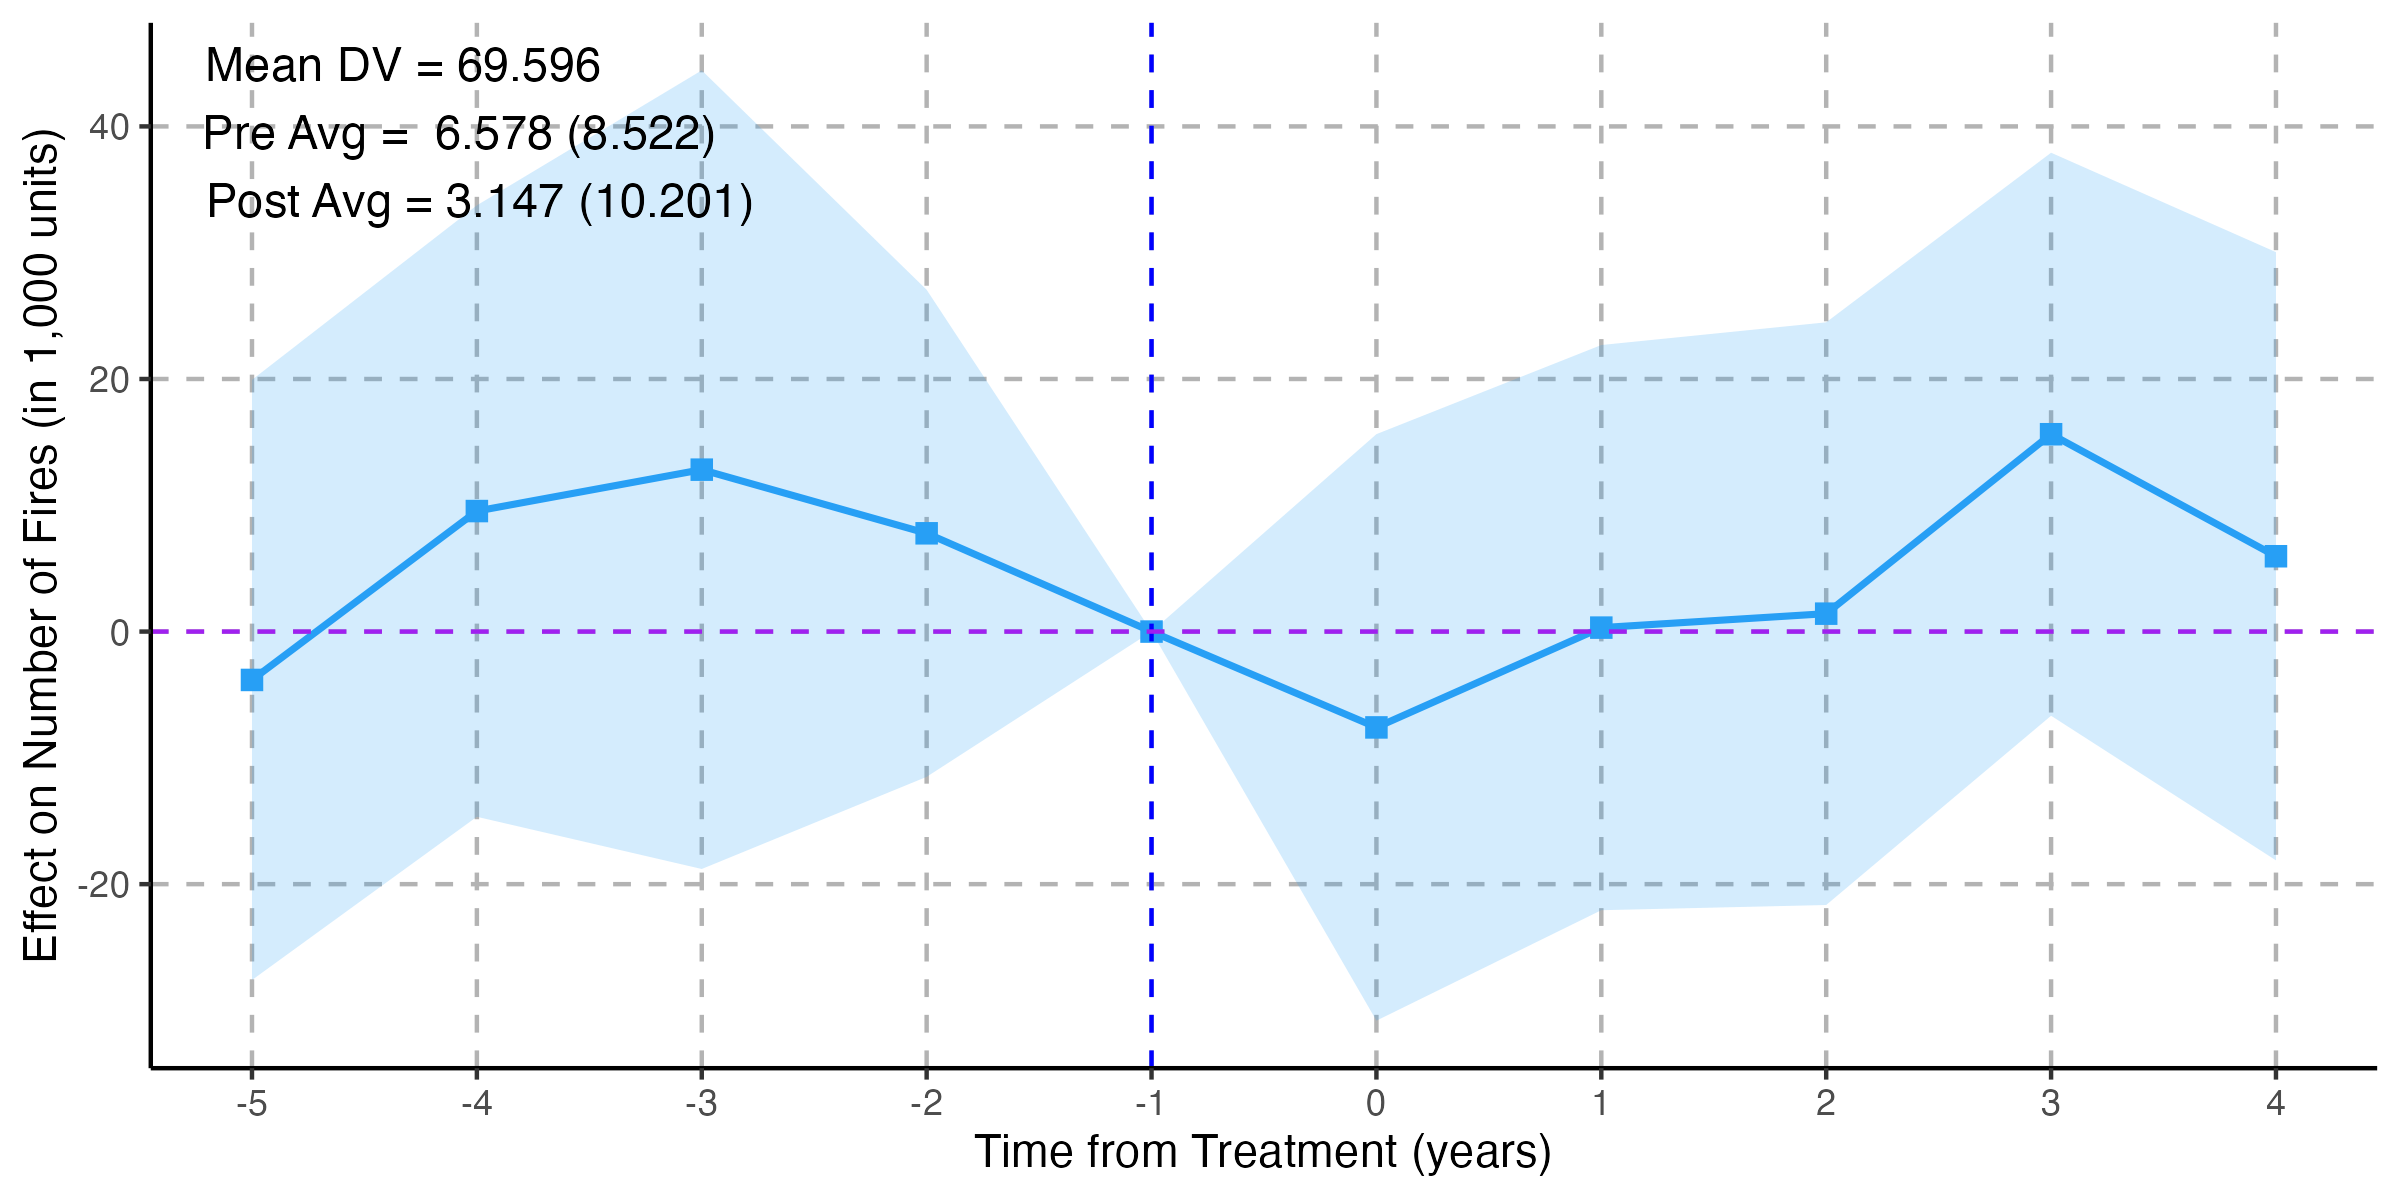
\includegraphics[width=0.85\linewidth]{../figures/app16_polischar_evst_fe1_ori.png}
\caption{Event study, original (fe1)}
\end{figure}
\begin{figure}[H]
\centering
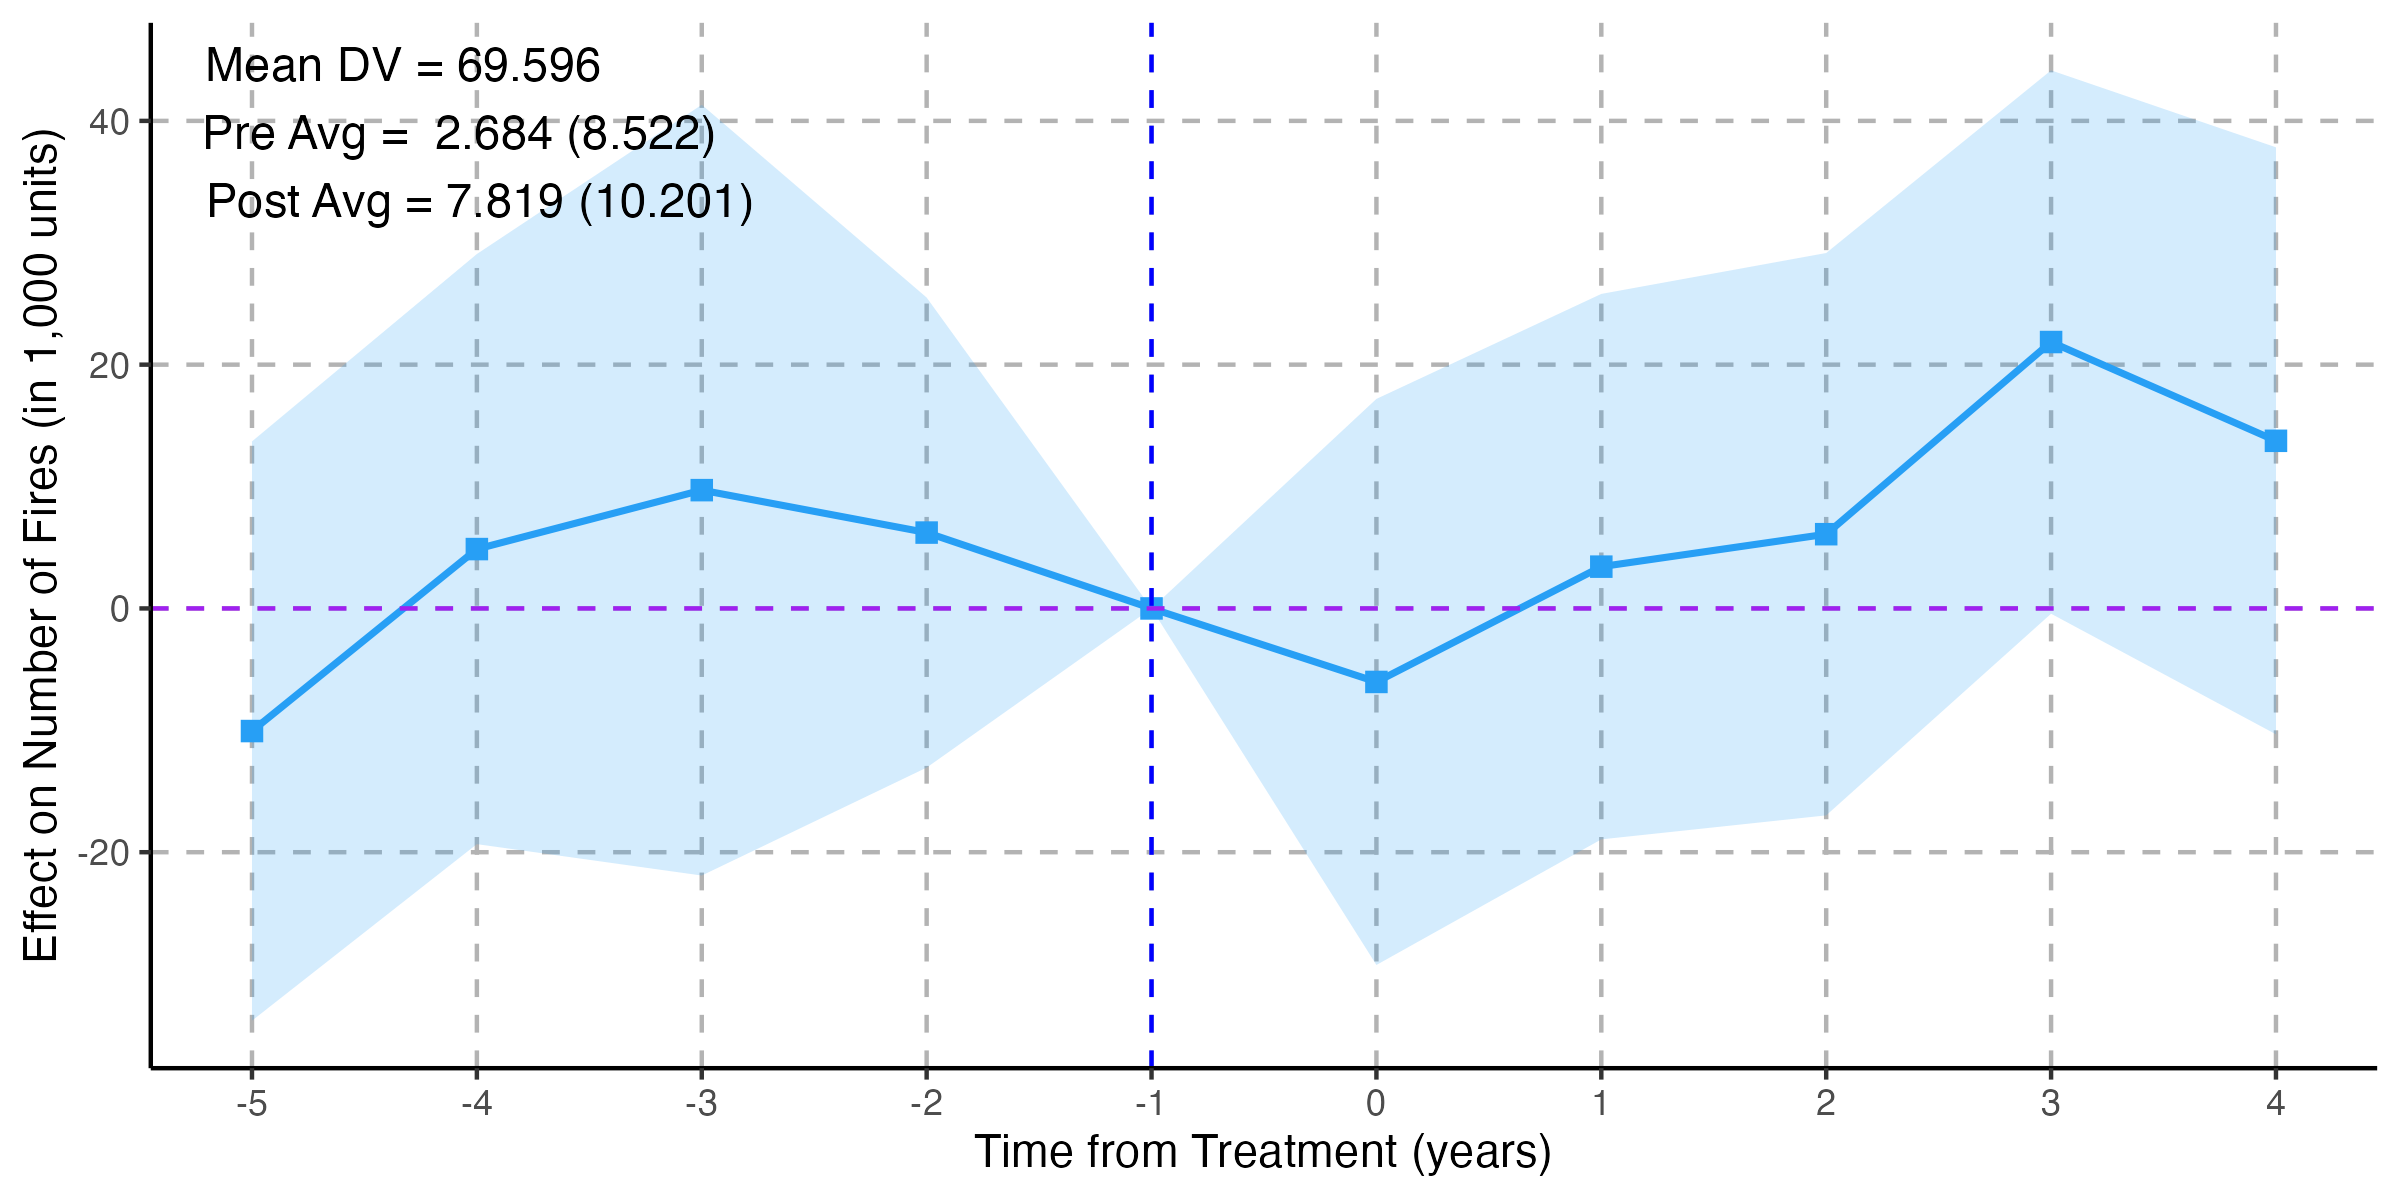
\includegraphics[width=0.85\linewidth]{../figures/app16_polischar_evst_fe1_rotated.png}
\caption{Event study, linear-detrended (fe1)}
\end{figure}
\subsection*{FE specification \texttt{fe8} (slot `evreg2')}
\begin{figure}[H]
\centering
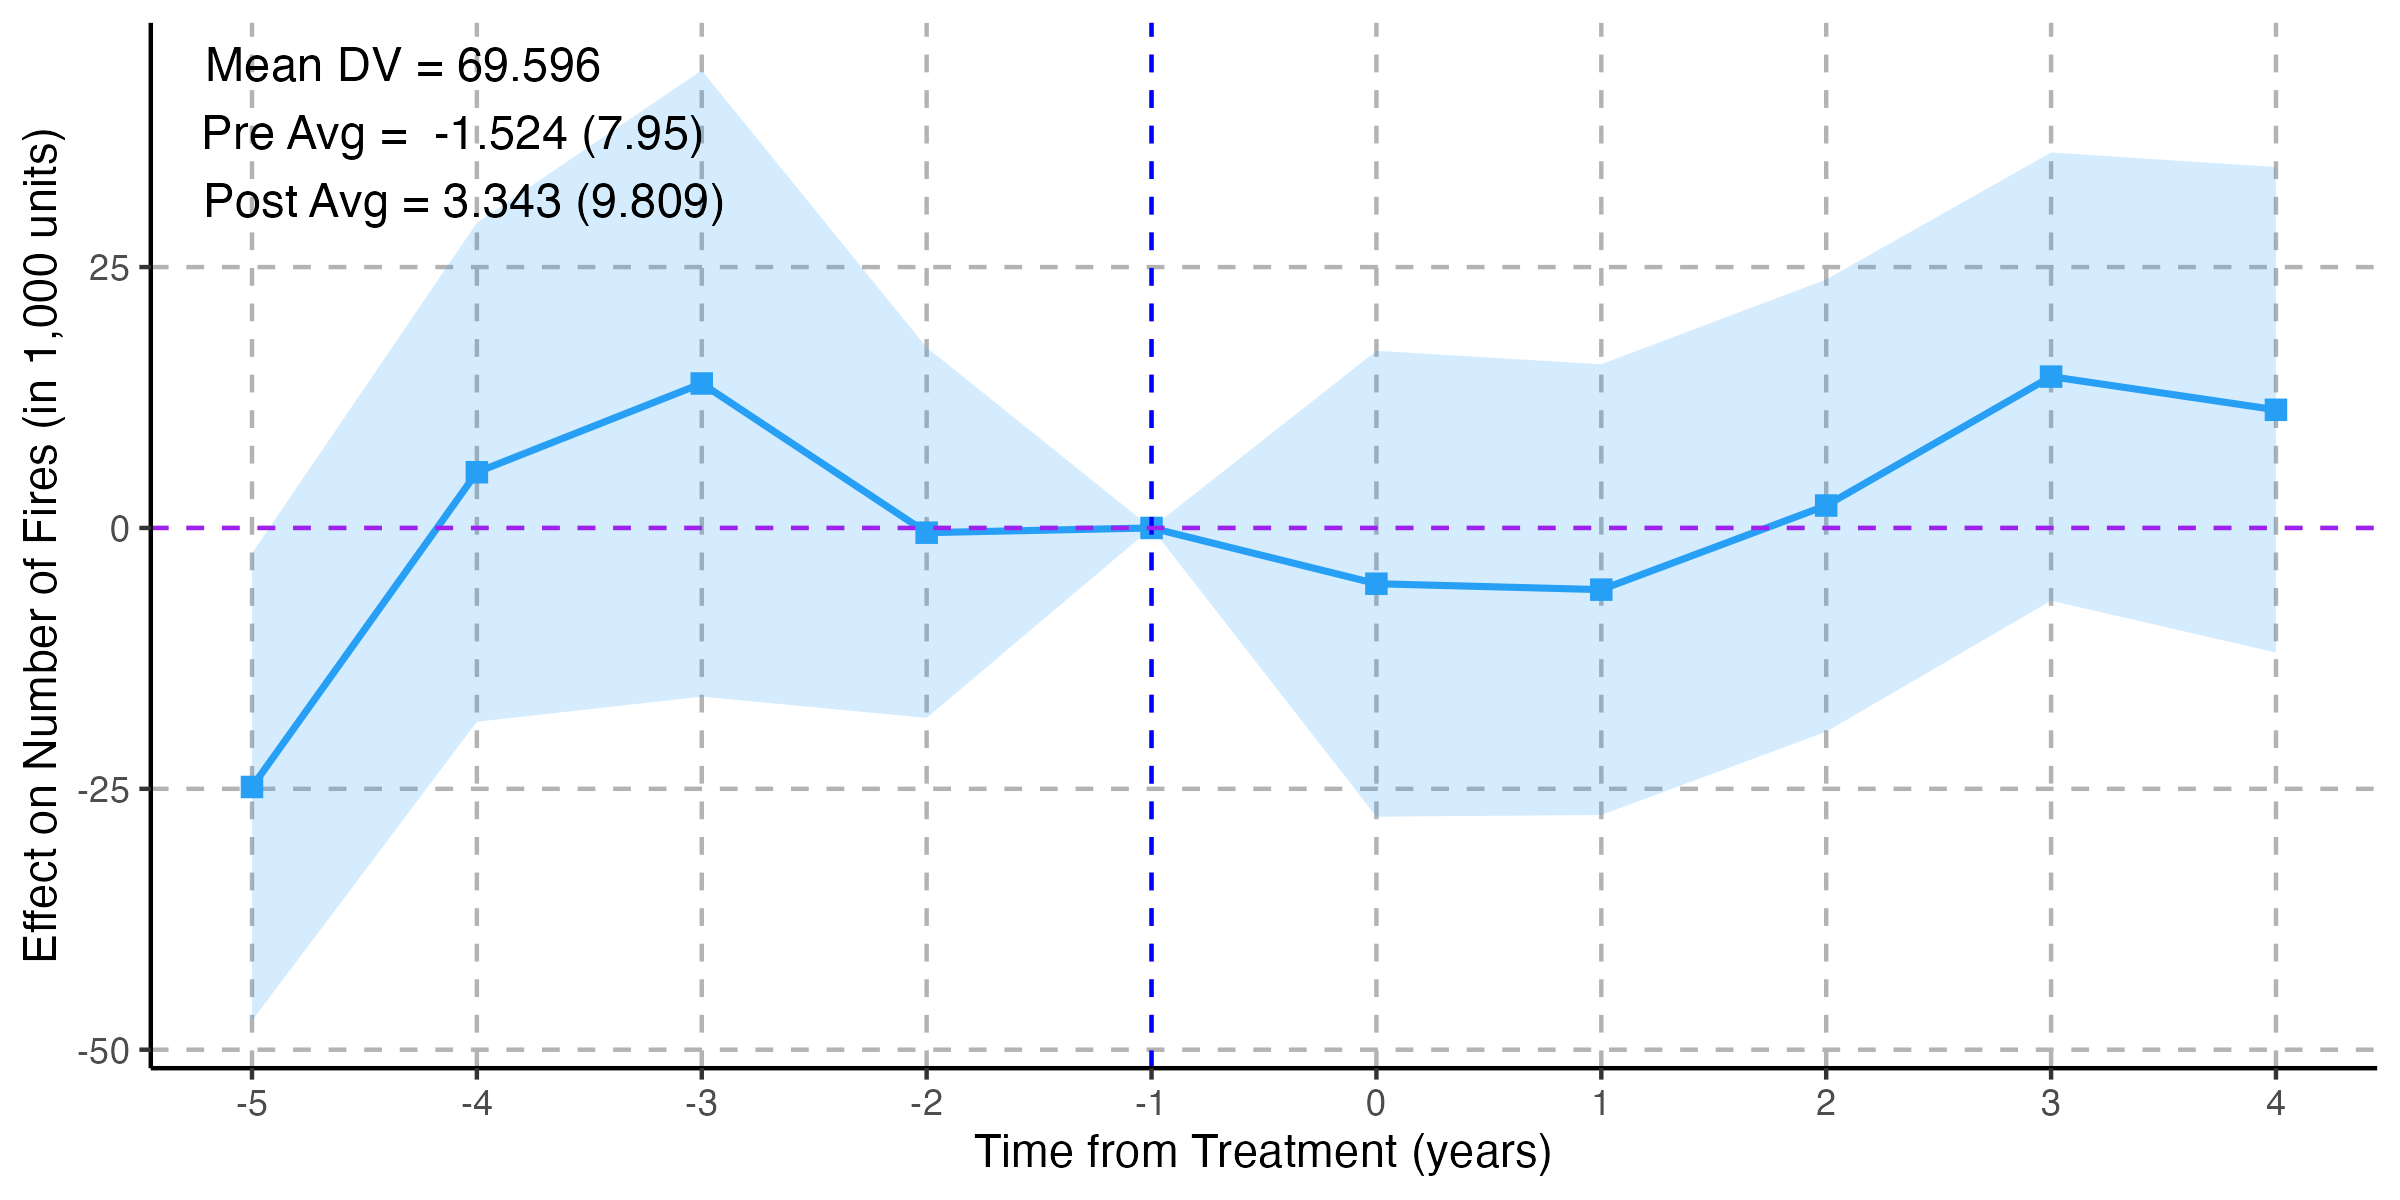
\includegraphics[width=0.85\linewidth]{../figures/app16_polischar_evst_fe8_ori.png}
\caption{Event study, original (fe8)}
\end{figure}
\begin{figure}[H]
\centering
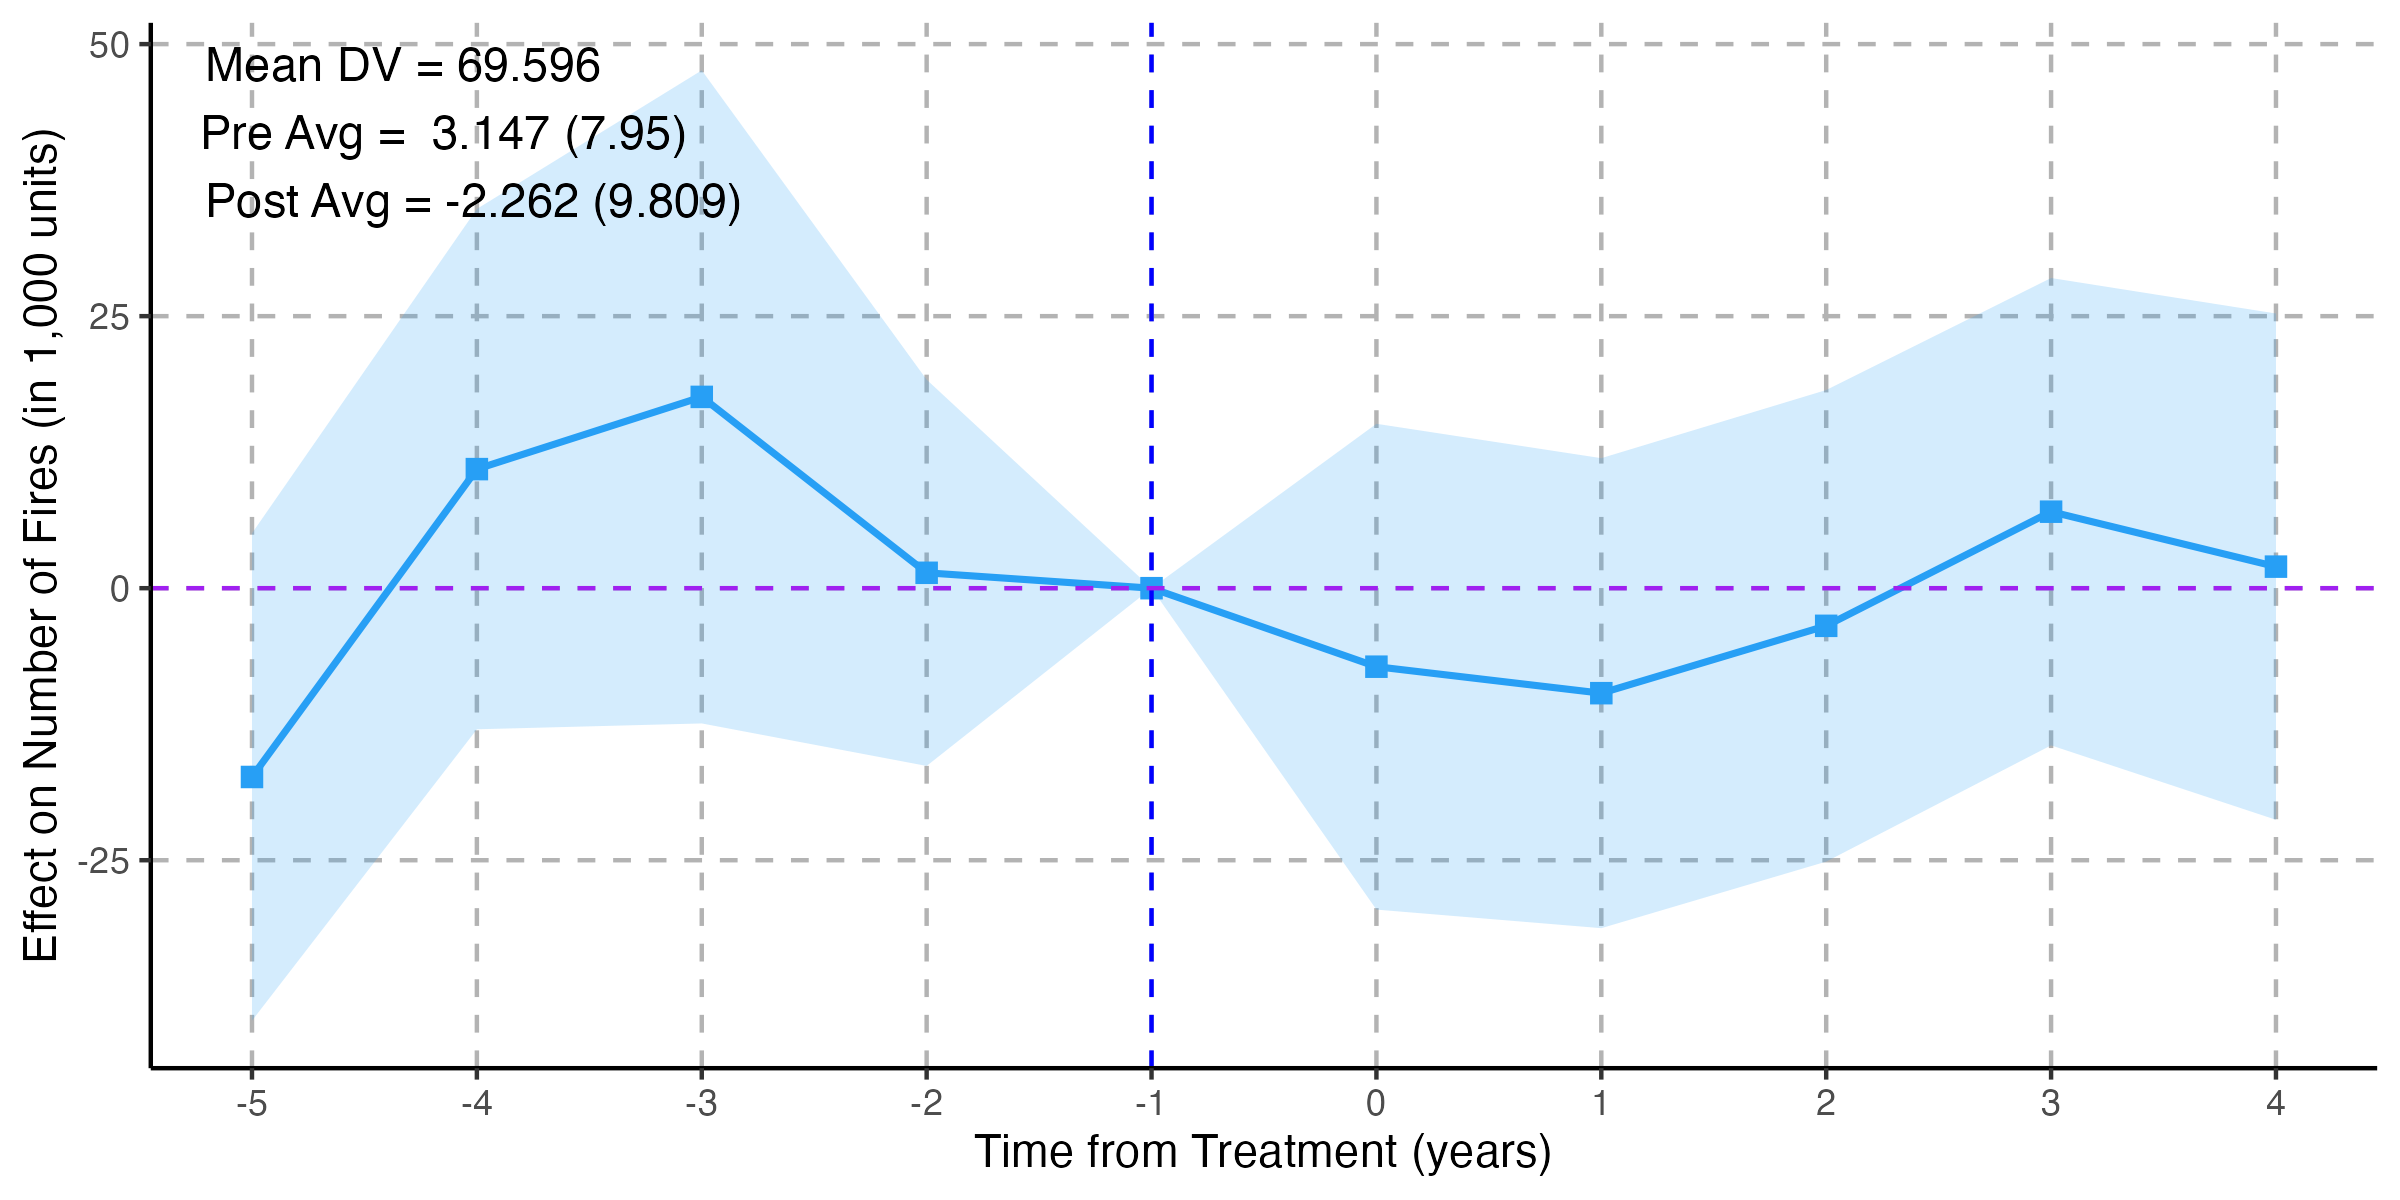
\includegraphics[width=0.85\linewidth]{../figures/app16_polischar_evst_fe8_rotated.png}
\caption{Event study, linear-detrended (fe8)}
\end{figure}
\subsection*{FE specification \texttt{fe16} (slot `evreg3')}
\begin{figure}[H]
\centering
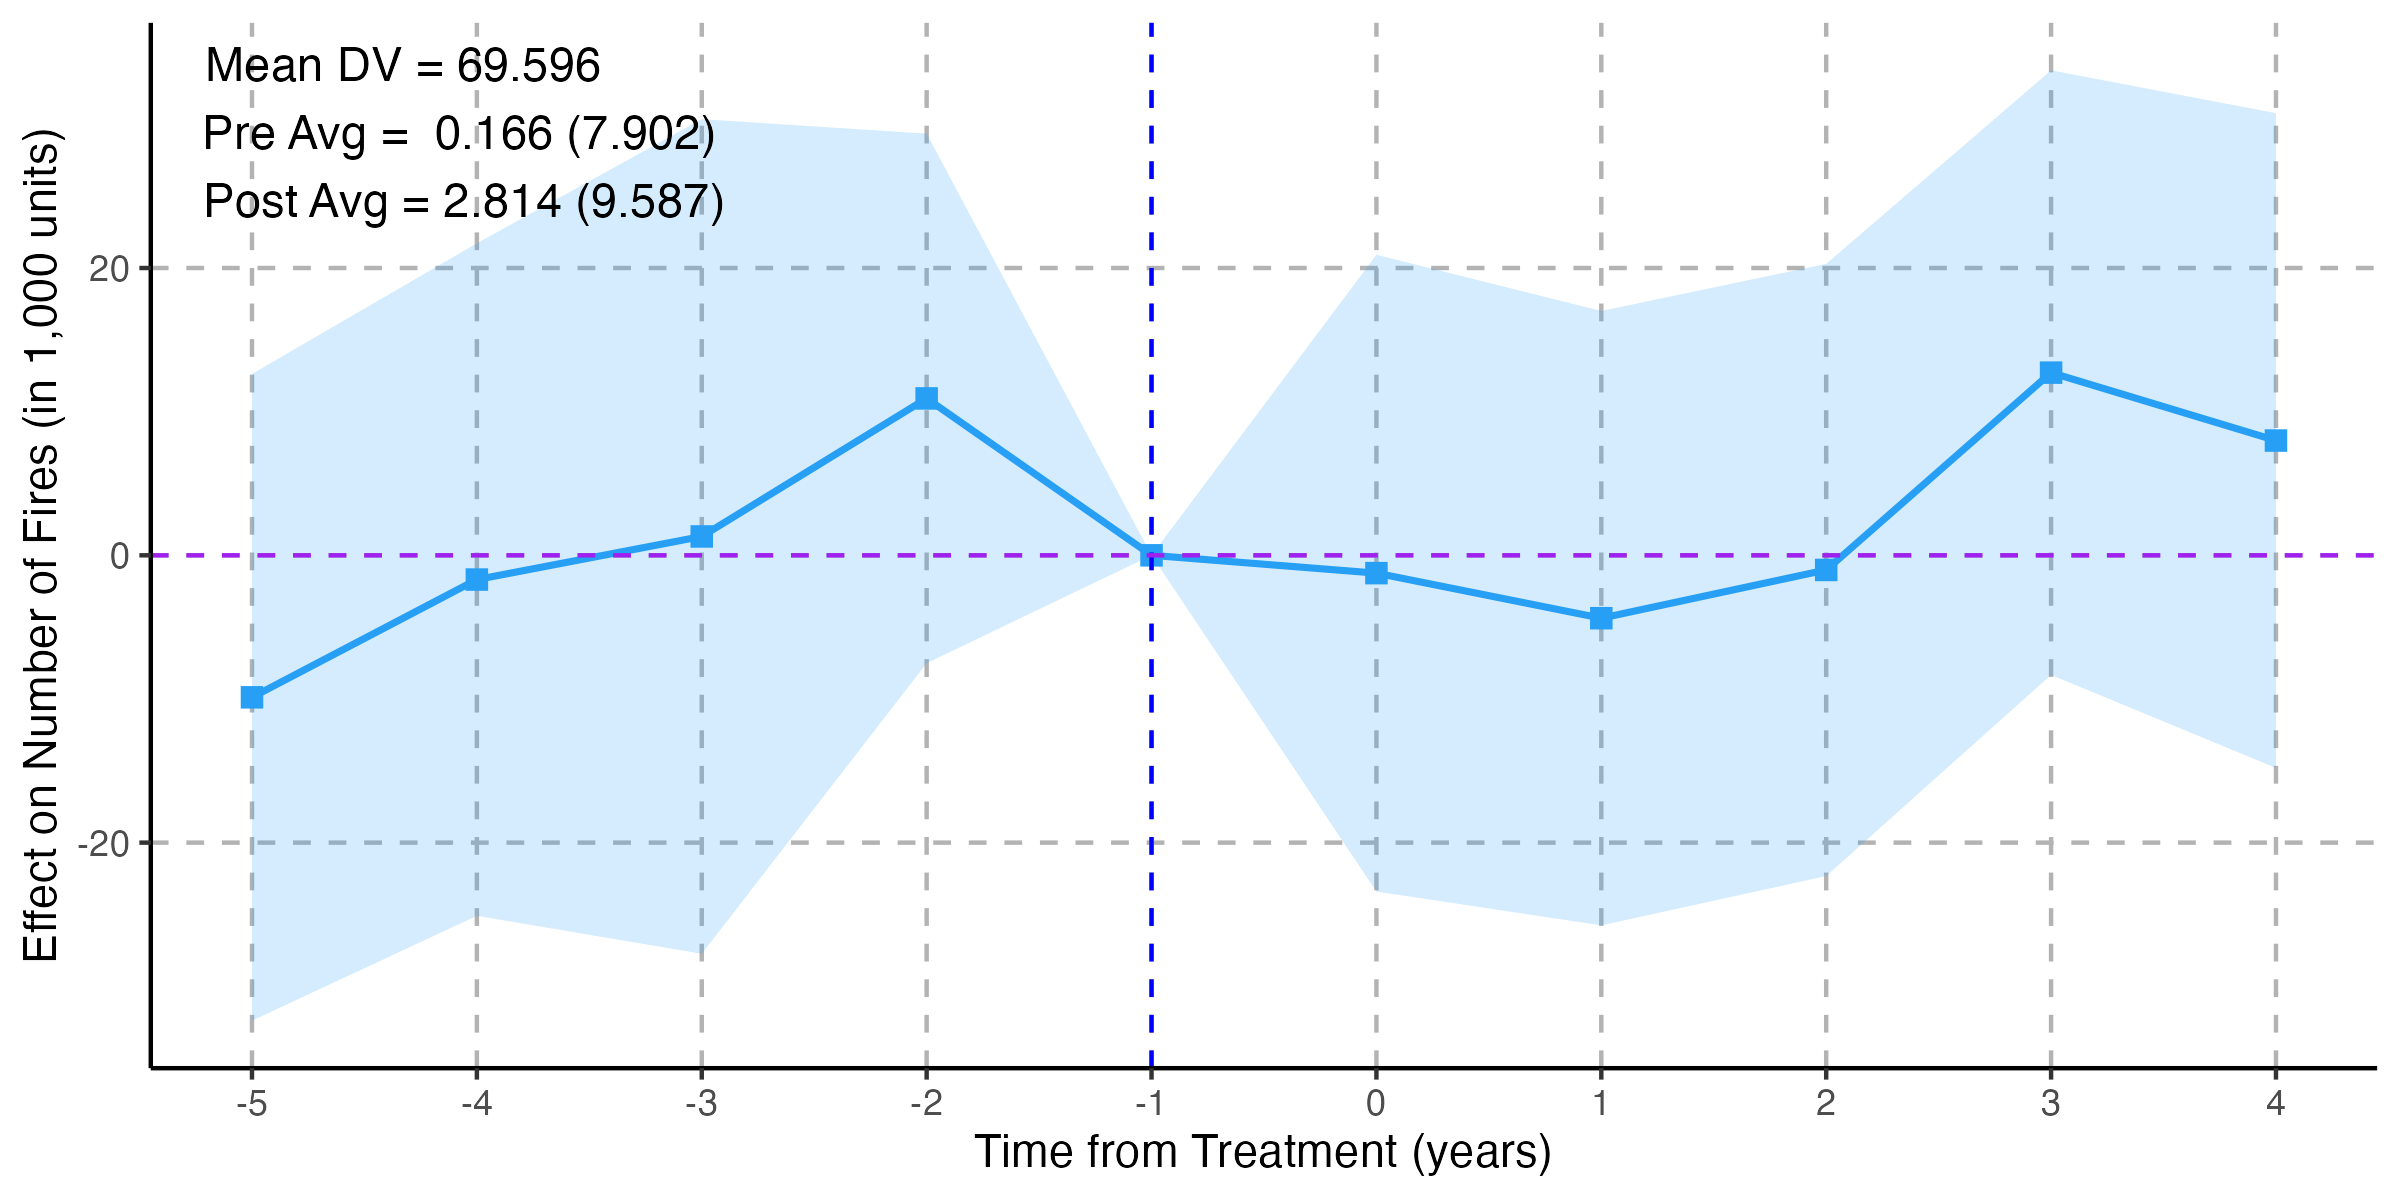
\includegraphics[width=0.85\linewidth]{../figures/app16_polischar_evst_fe16_ori.png}
\caption{Event study, original (fe16)}
\end{figure}
\begin{figure}[H]
\centering
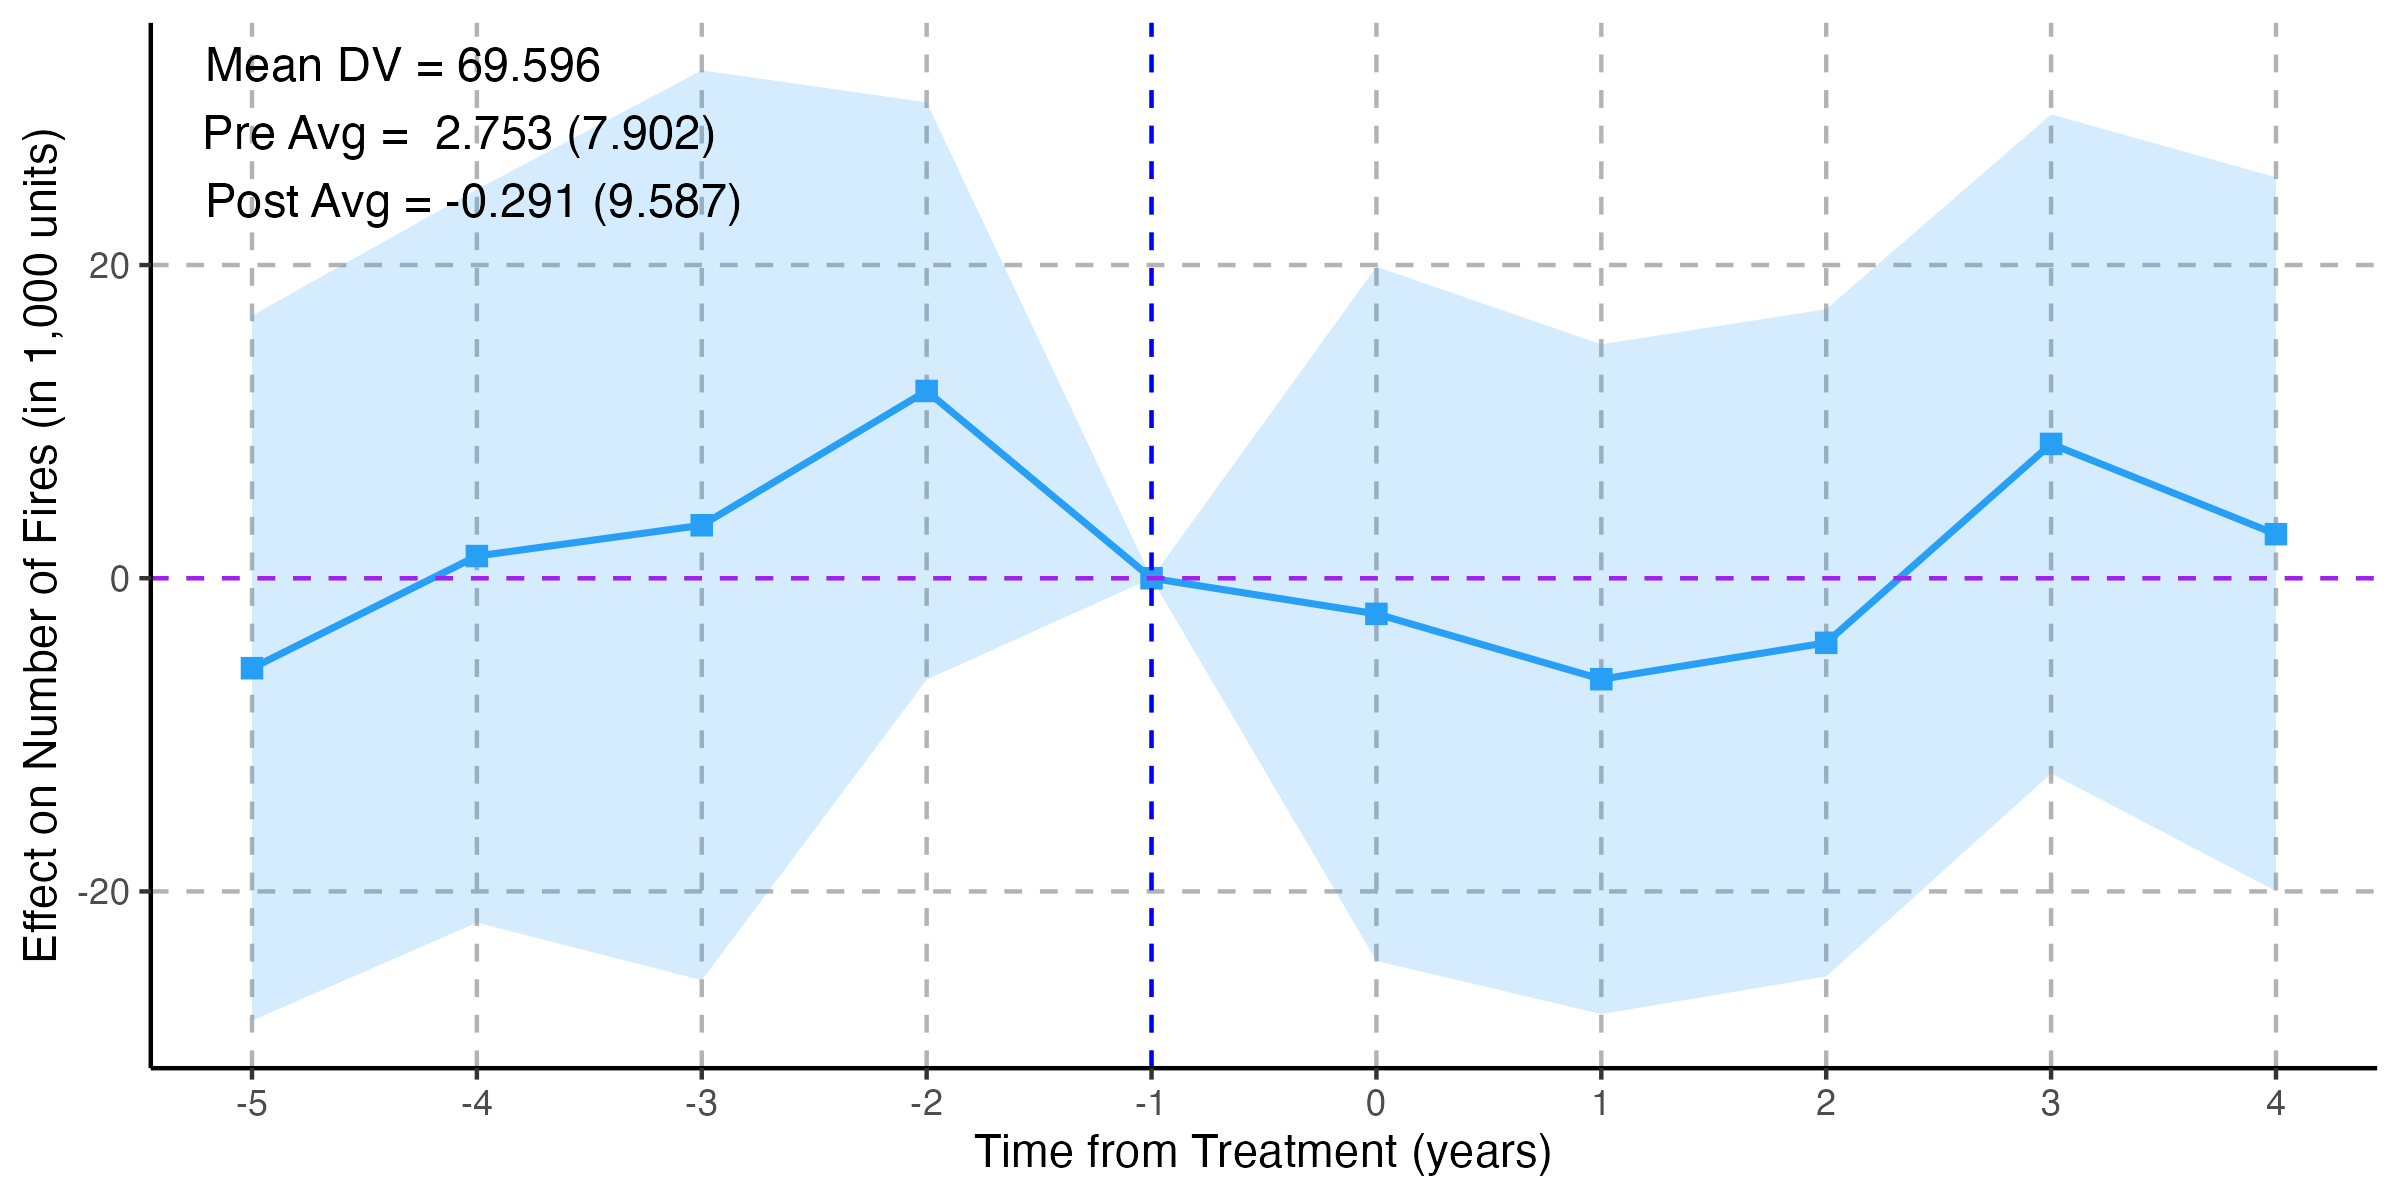
\includegraphics[width=0.85\linewidth]{../figures/app16_polischar_evst_fe16_rotated.png}
\caption{Event study, linear-detrended (fe16)}
\end{figure}
\subsection*{FE specification \texttt{fe24} (slot `evreg4')}
\begin{figure}[H]
\centering
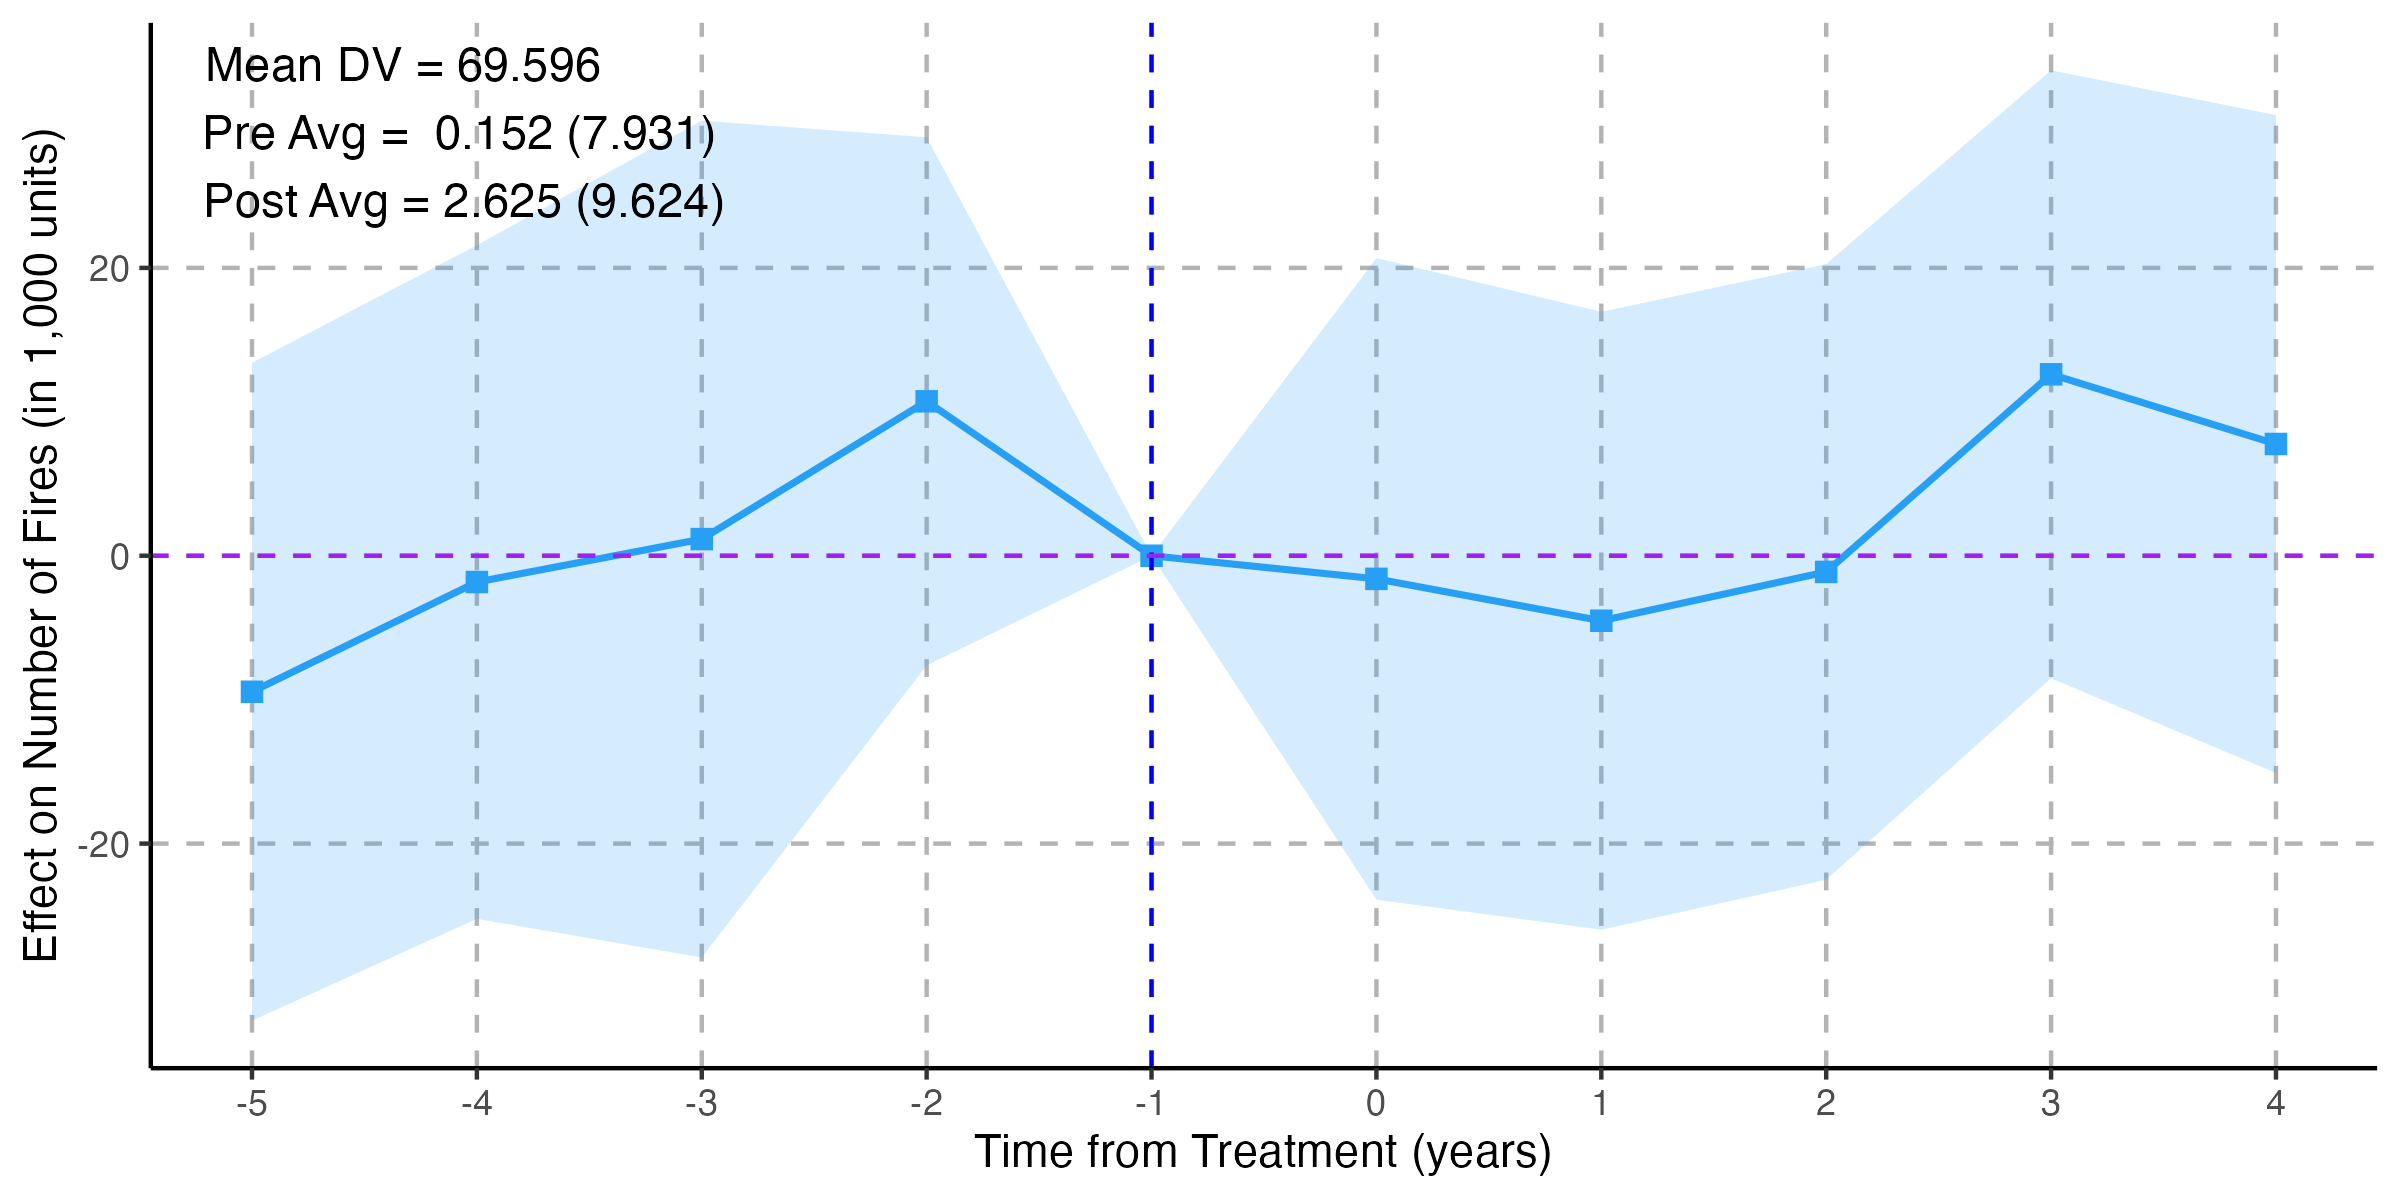
\includegraphics[width=0.85\linewidth]{../figures/app16_polischar_evst_fe24_ori.png}
\caption{Event study, original (fe24)}
\end{figure}
\begin{figure}[H]
\centering
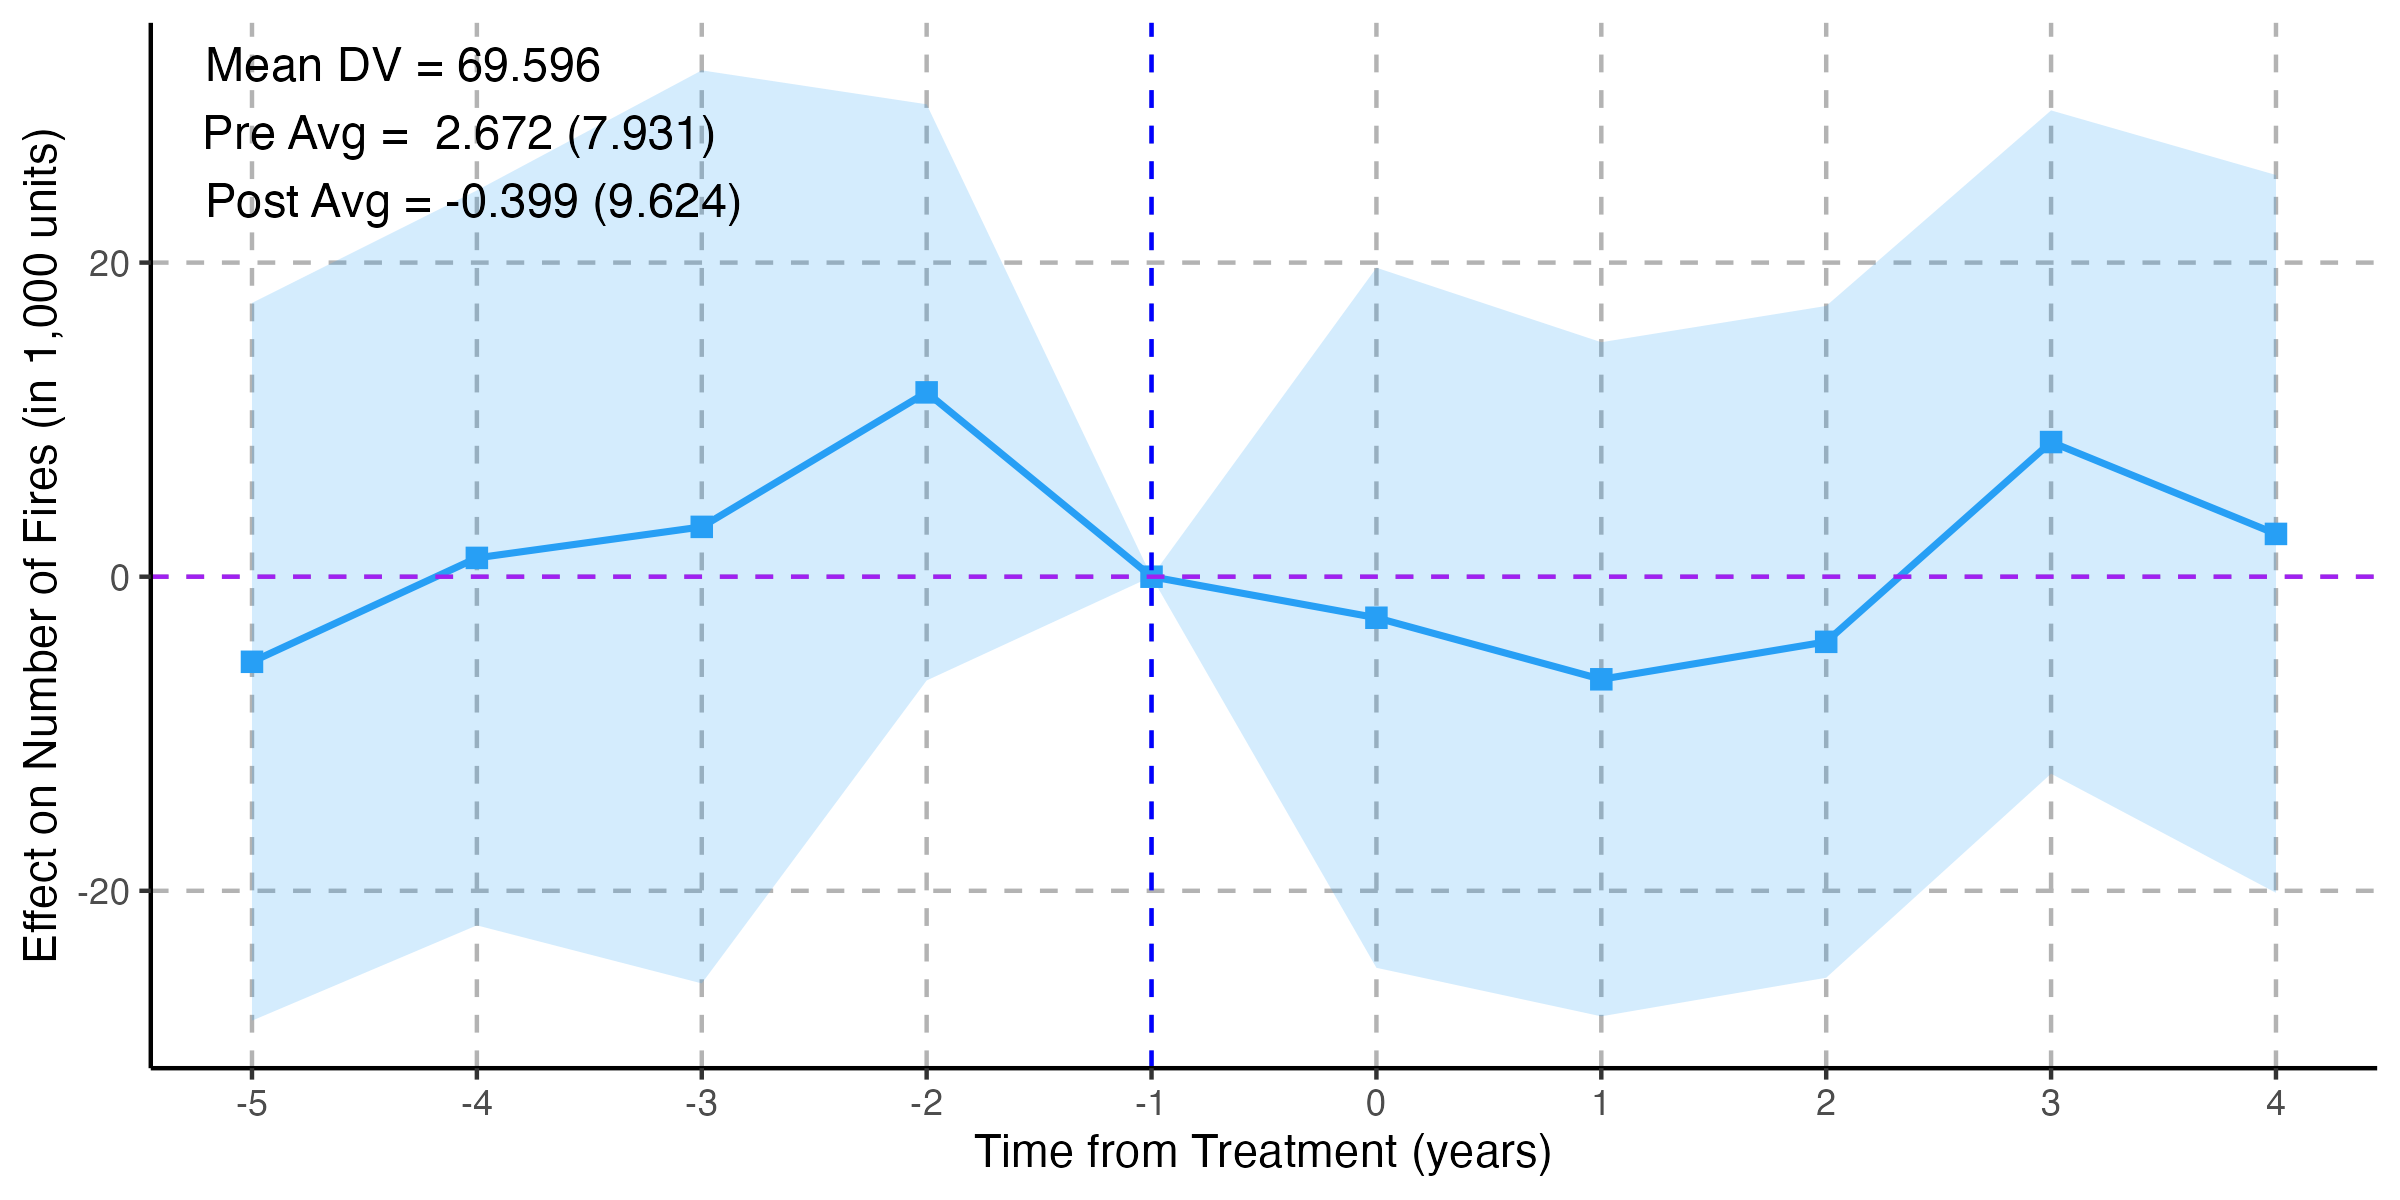
\includegraphics[width=0.85\linewidth]{../figures/app16_polischar_evst_fe24_rotated.png}
\caption{Event study, linear-detrended (fe24)}
\end{figure}
\subsection*{FE specification \texttt{fe32} (slot `evreg5')}
\begin{figure}[H]
\centering
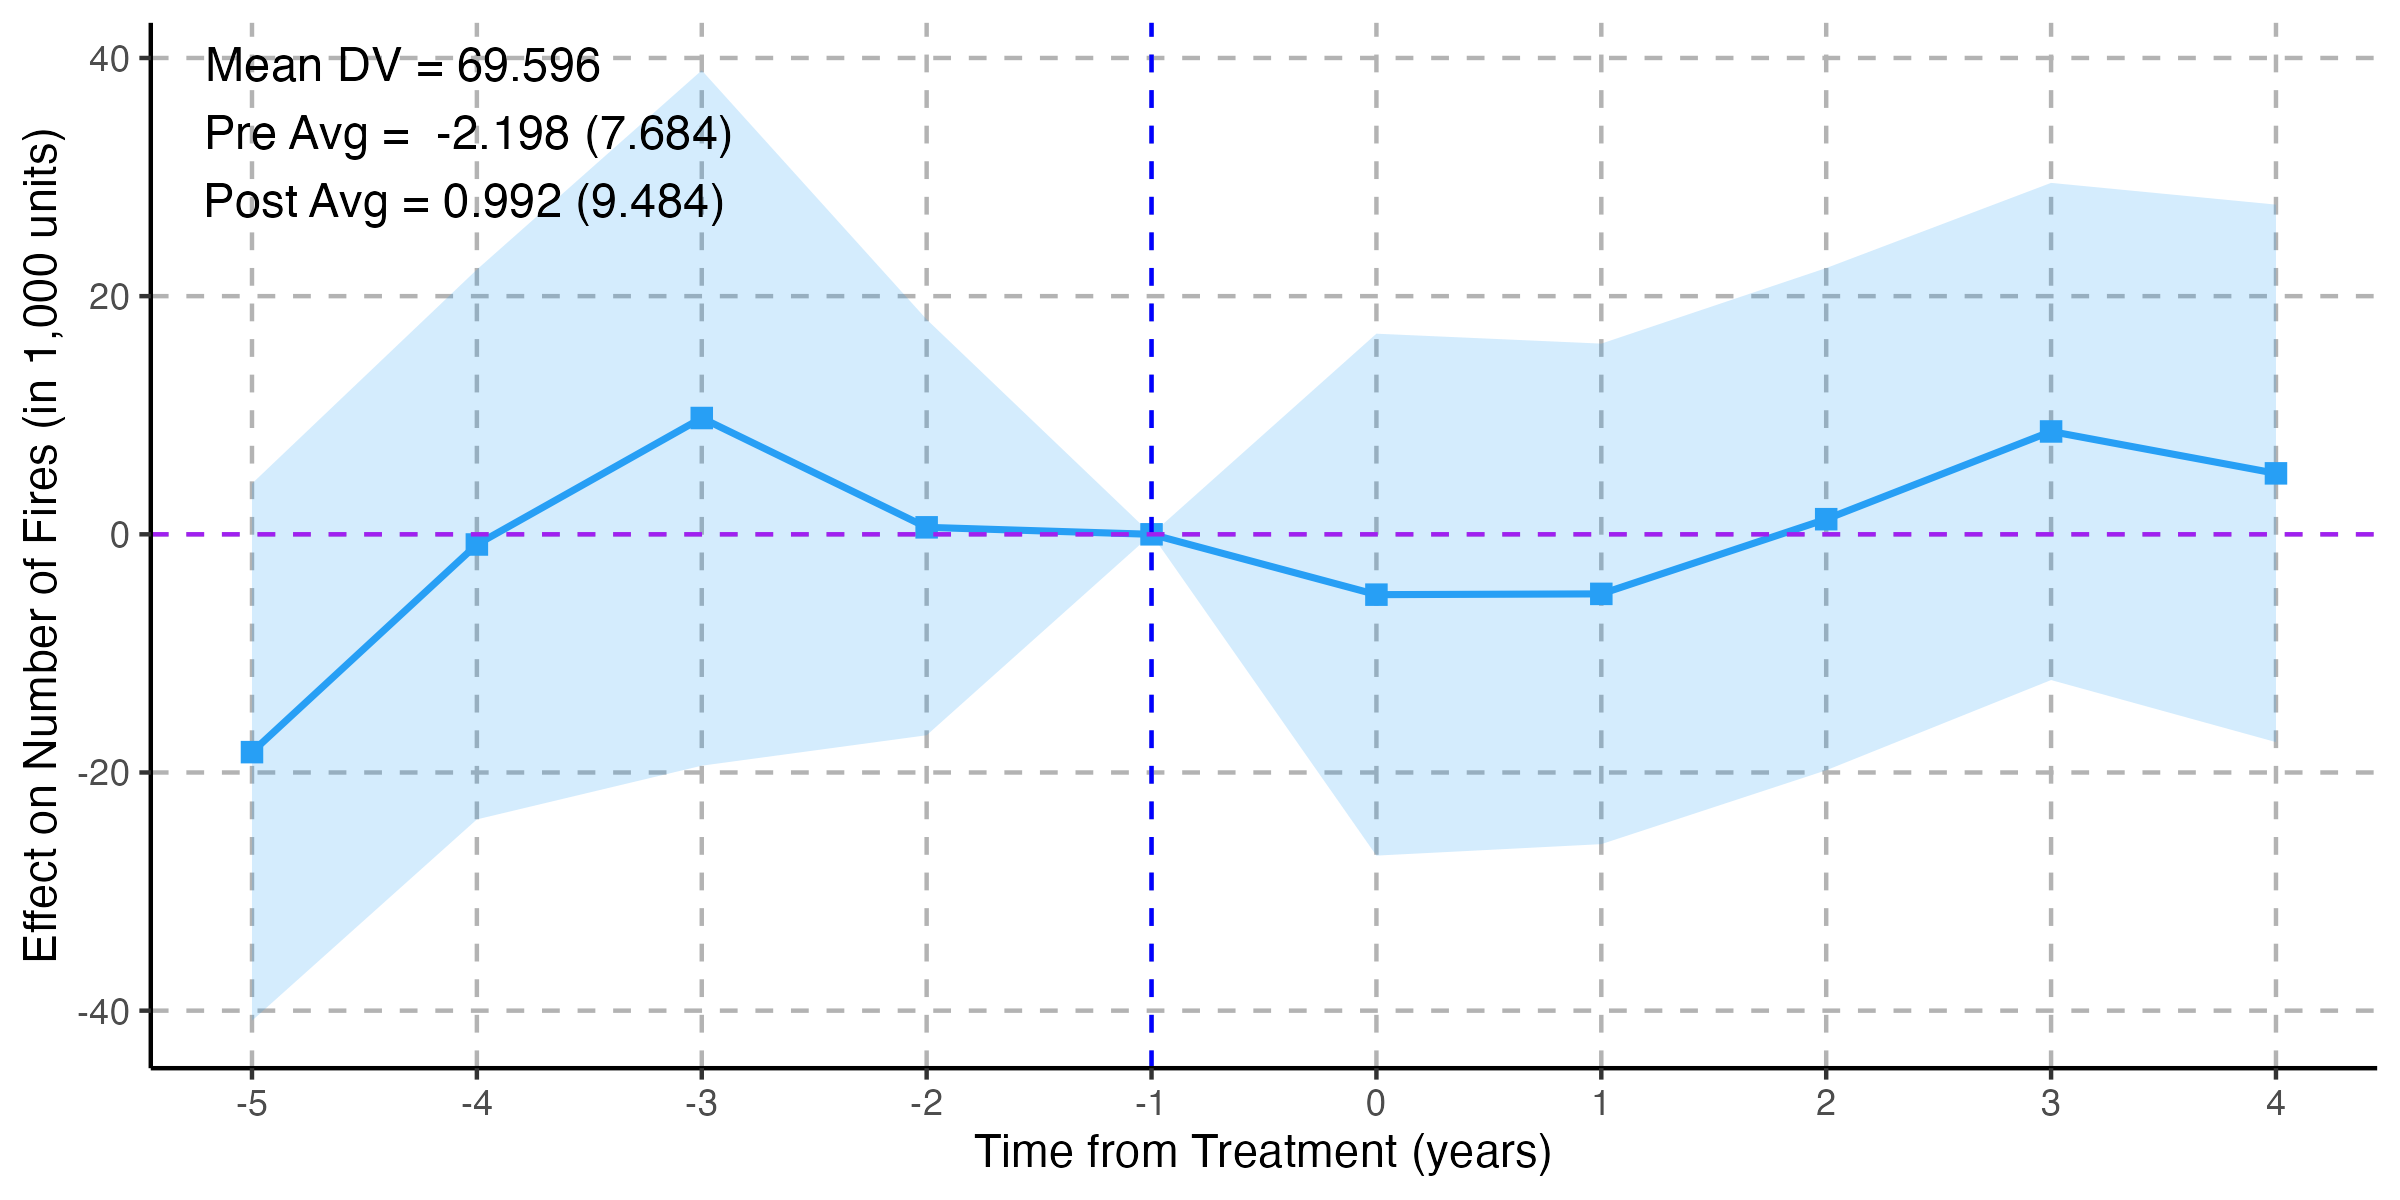
\includegraphics[width=0.85\linewidth]{../figures/app16_polischar_evst_fe32_ori.png}
\caption{Event study, original (fe32)}
\end{figure}
\begin{figure}[H]
\centering
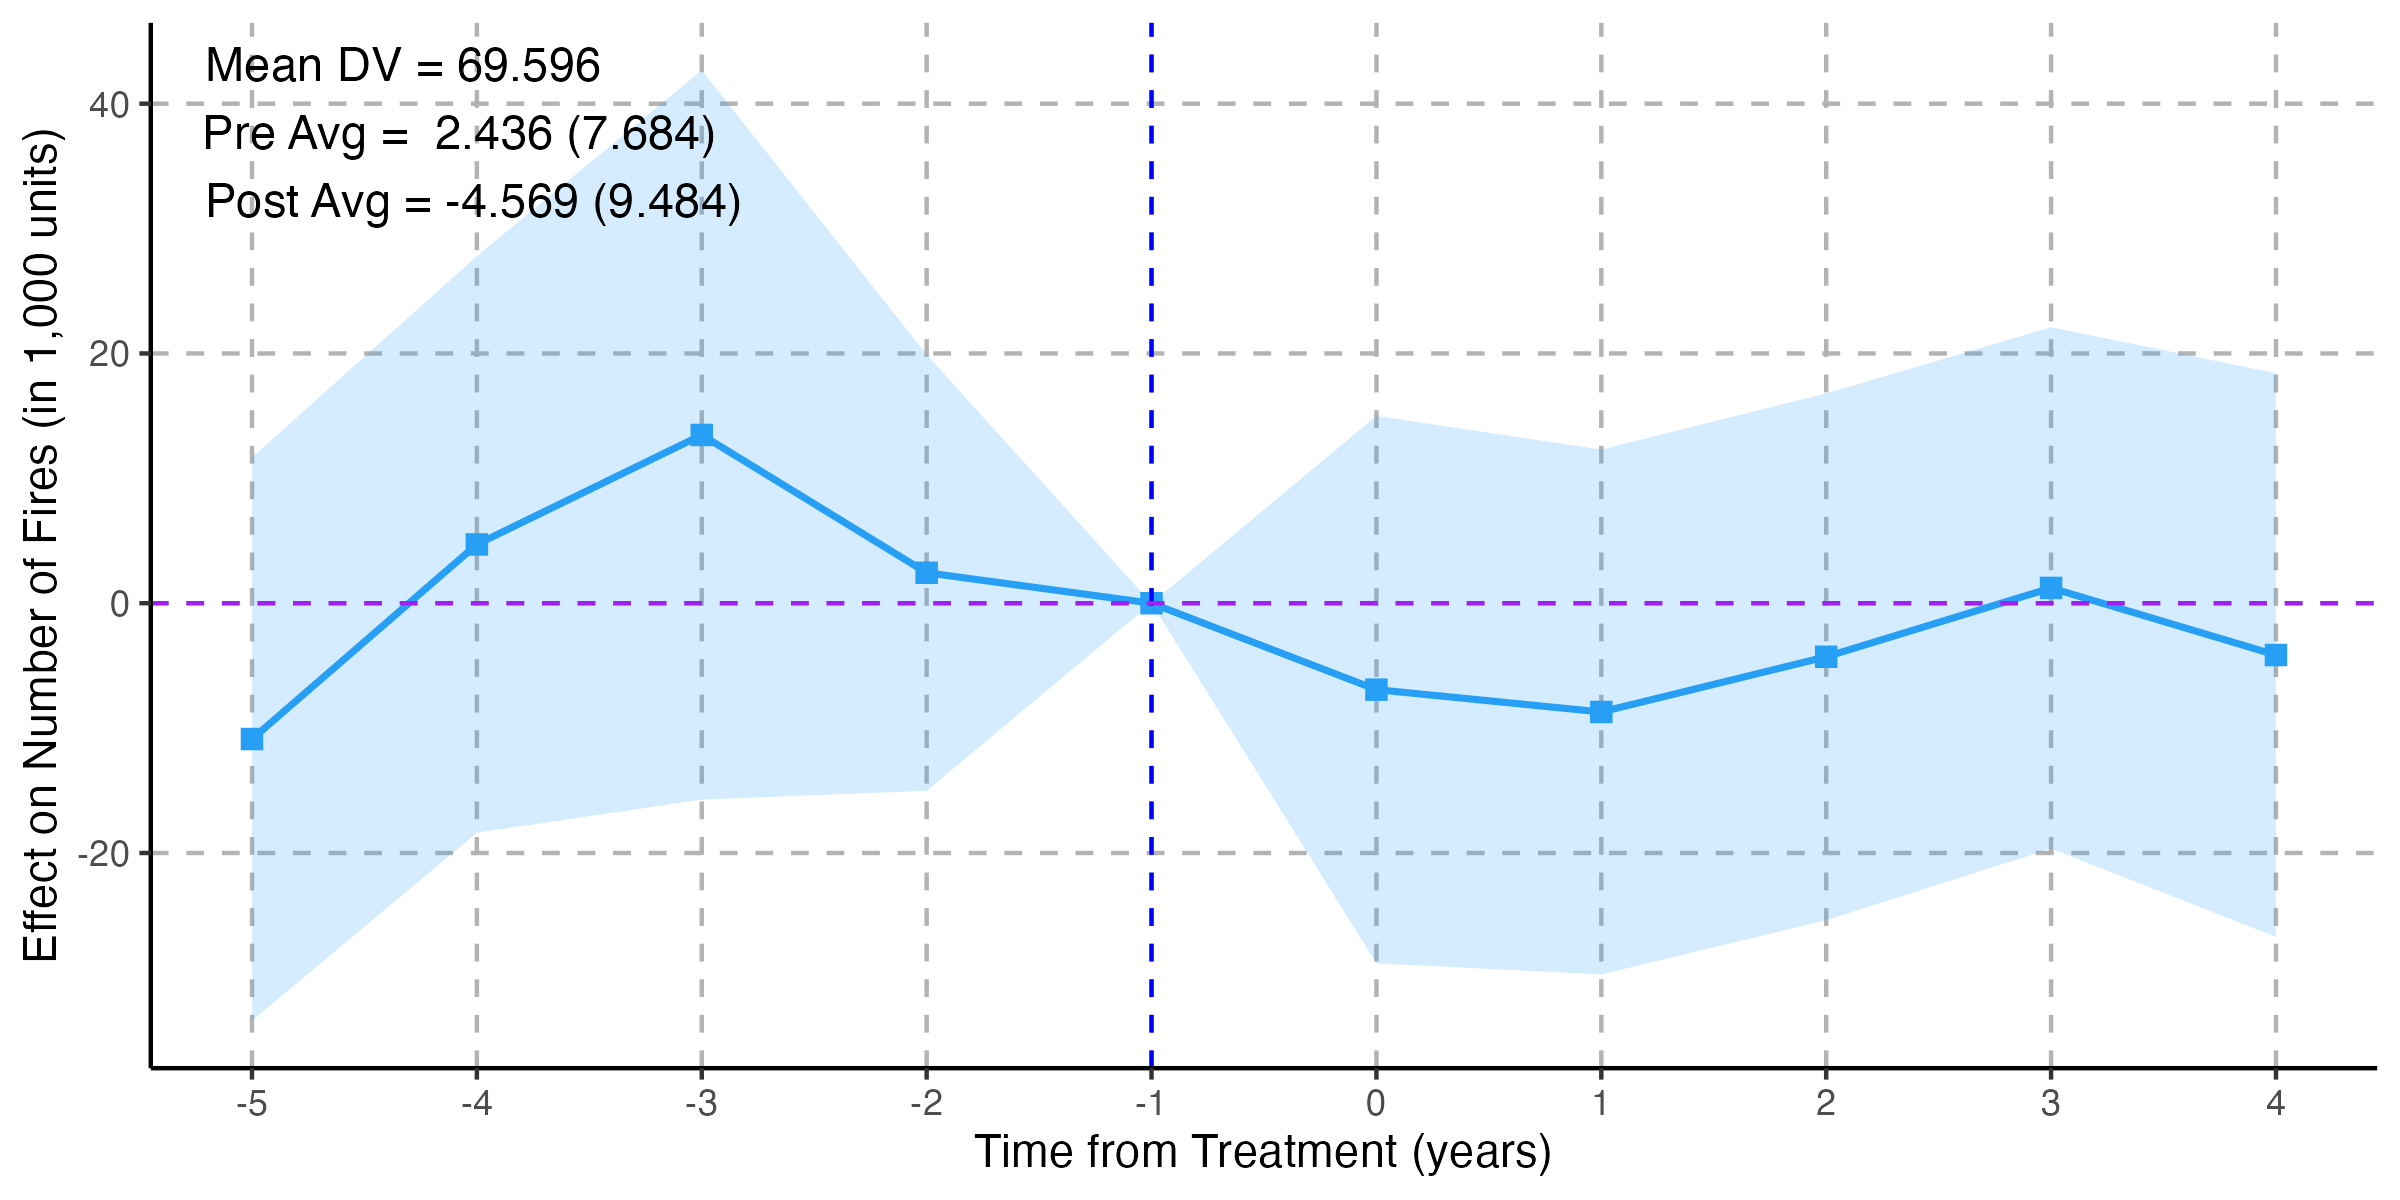
\includegraphics[width=0.85\linewidth]{../figures/app16_polischar_evst_fe32_rotated.png}
\caption{Event study, linear-detrended (fe32)}
\end{figure}
\FloatBarrier
\clearpage
\section{Event studies --- Protest (\texttt{\_app\_17})}
Dependent variable: fires per 1{,}000 units. Base event period: $t = 0$.
\subsection*{FE specification \texttt{fe1} (slot `evreg1')}
\begin{figure}[H]
\centering
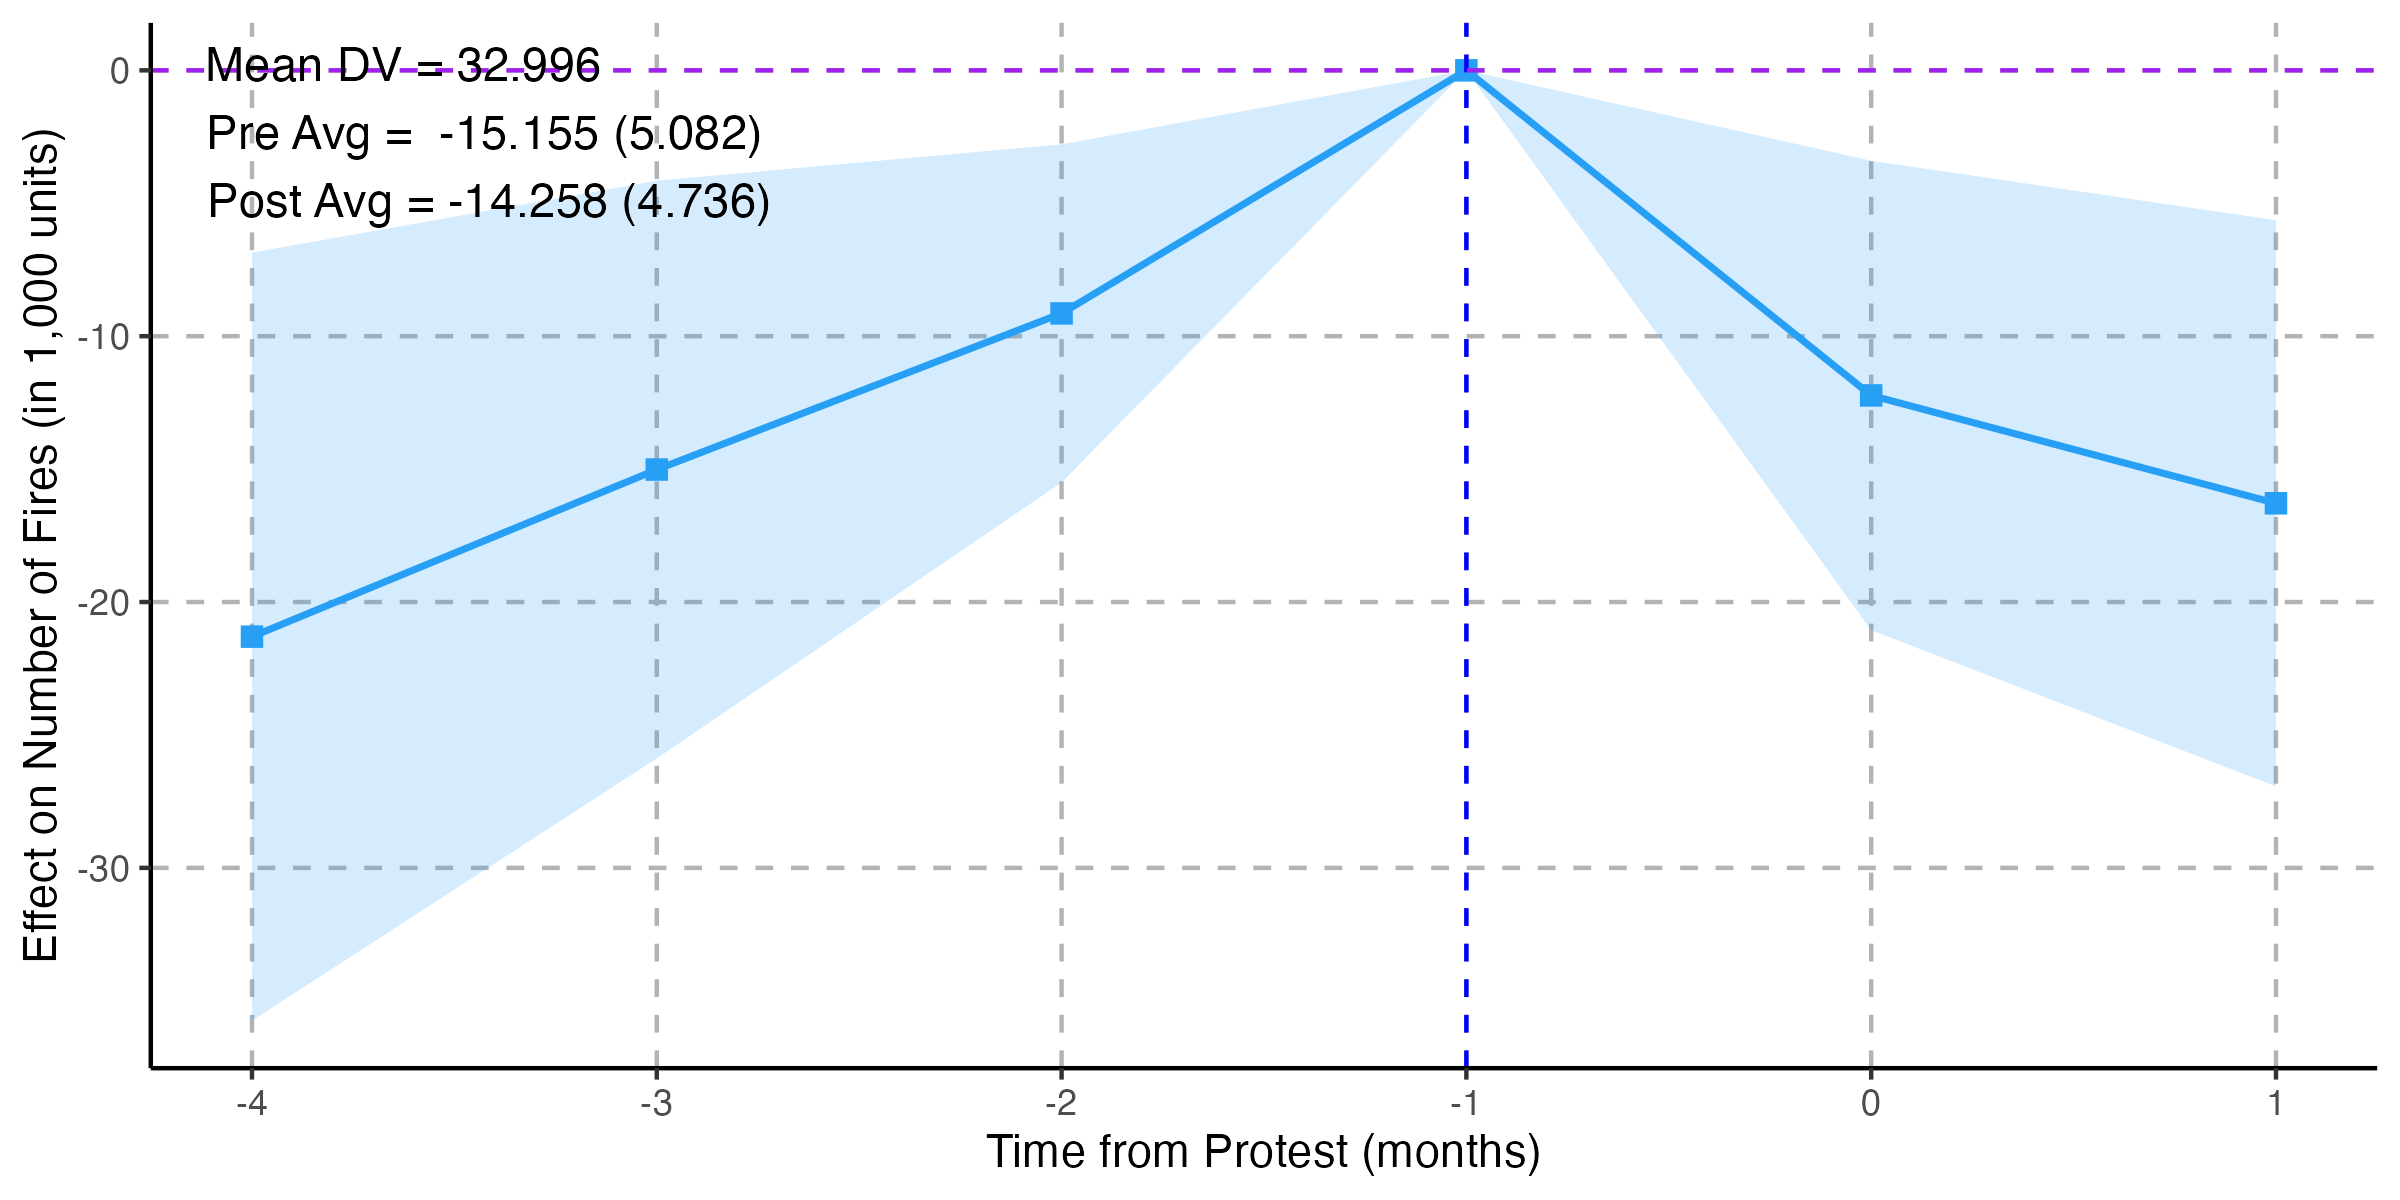
\includegraphics[width=0.85\linewidth]{../figures/app17_protest_evst_fe1_ori.png}
\caption{Event study, original (fe1)}
\end{figure}
\begin{figure}[H]
\centering
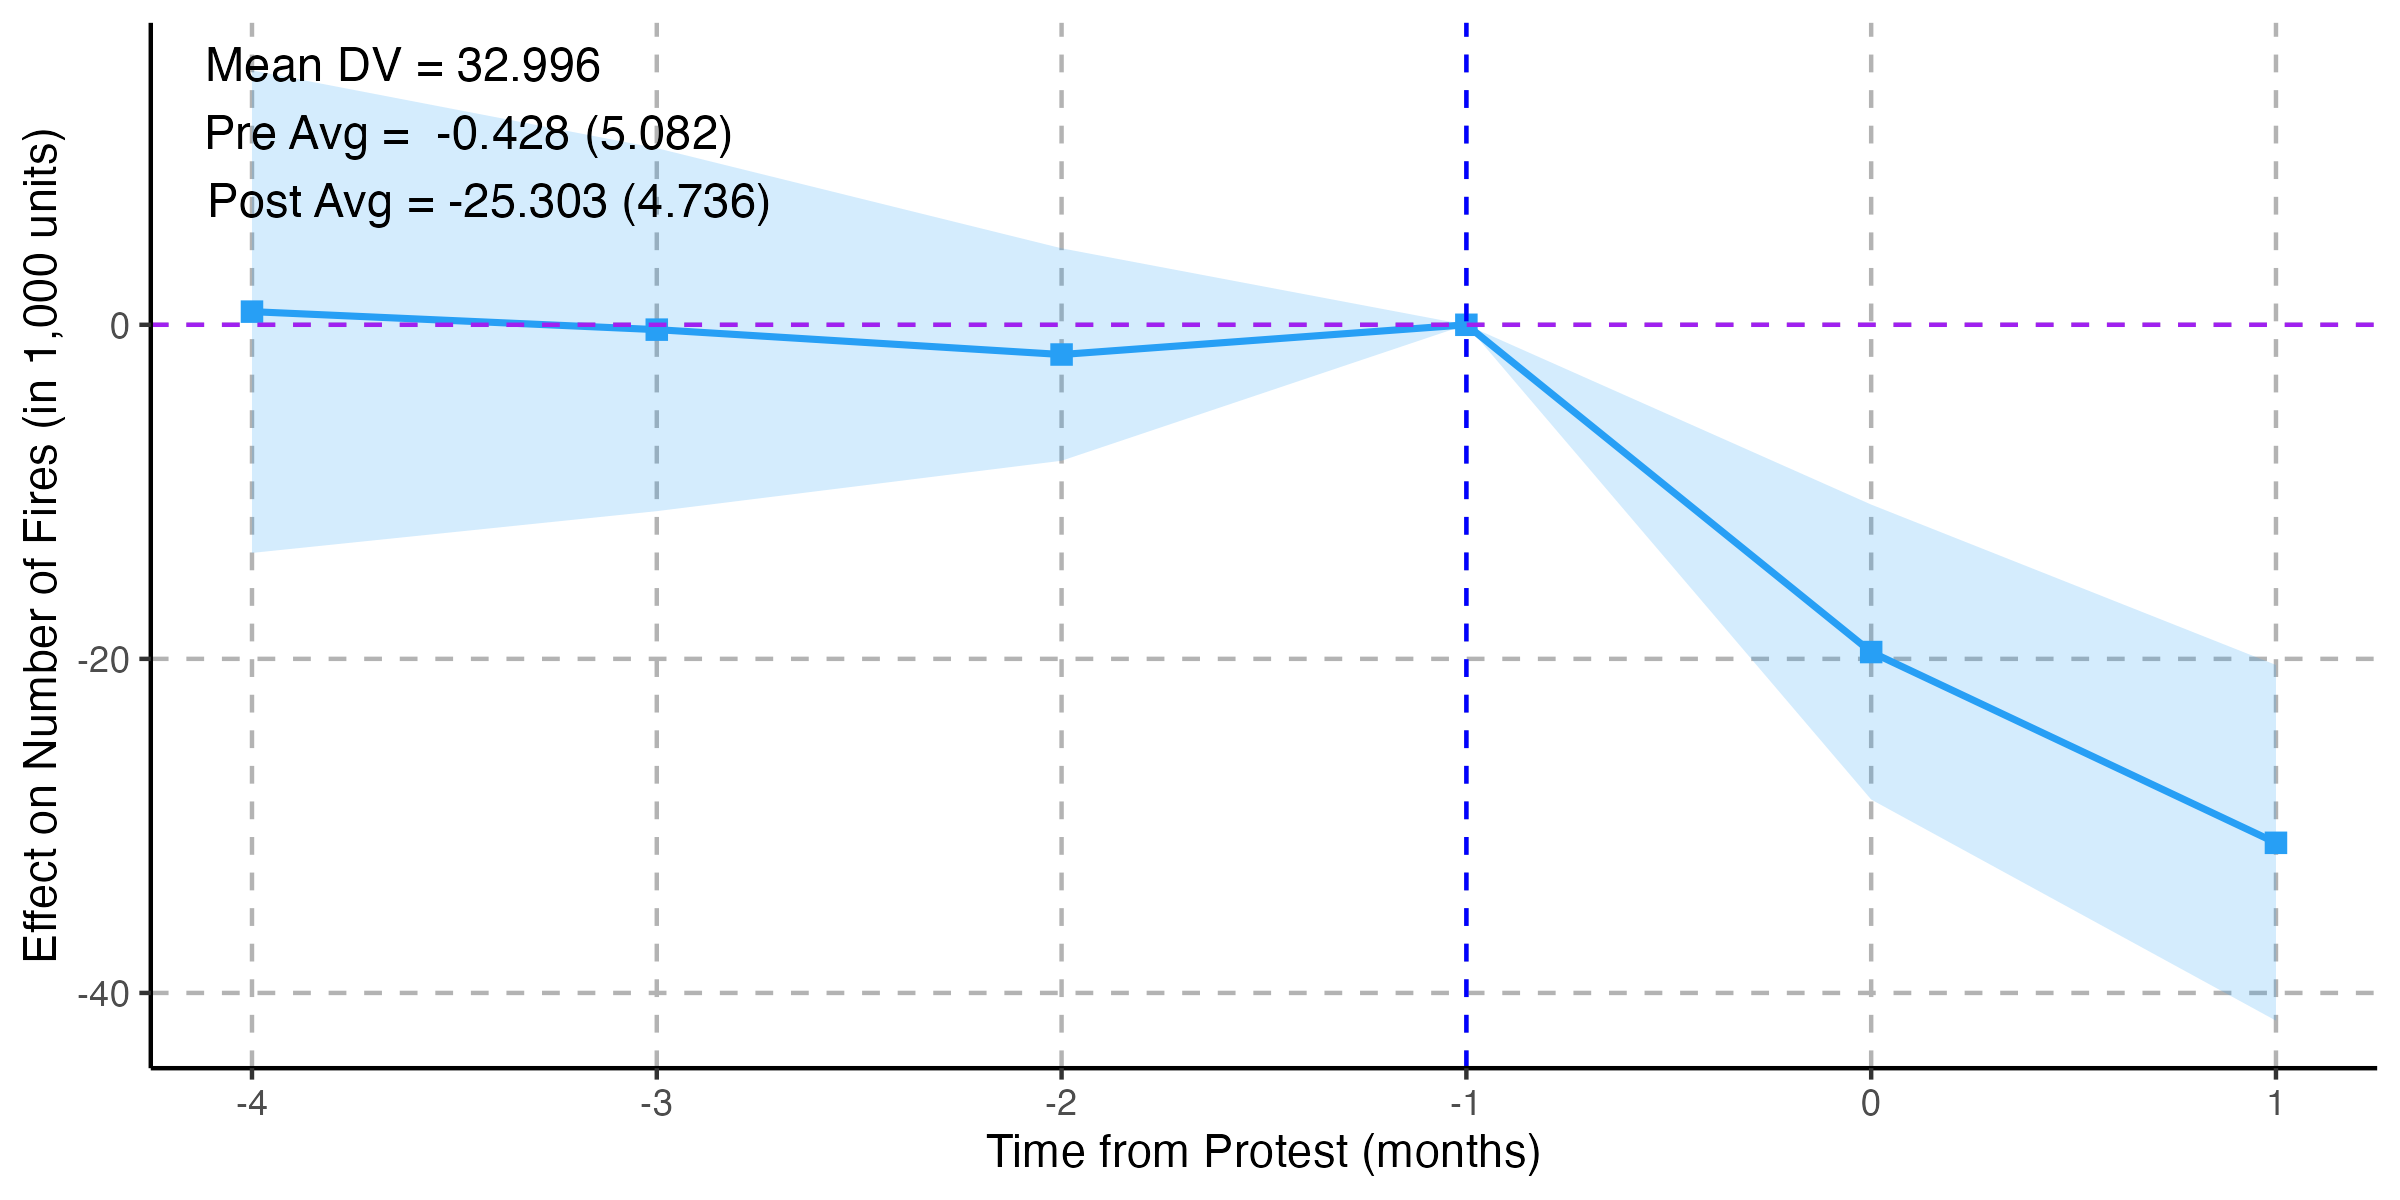
\includegraphics[width=0.85\linewidth]{../figures/app17_protest_evst_fe1_rotated.png}
\caption{Event study, linear-detrended (fe1)}
\end{figure}
\subsection*{FE specification \texttt{fe8} (slot `evreg2')}
\begin{figure}[H]
\centering
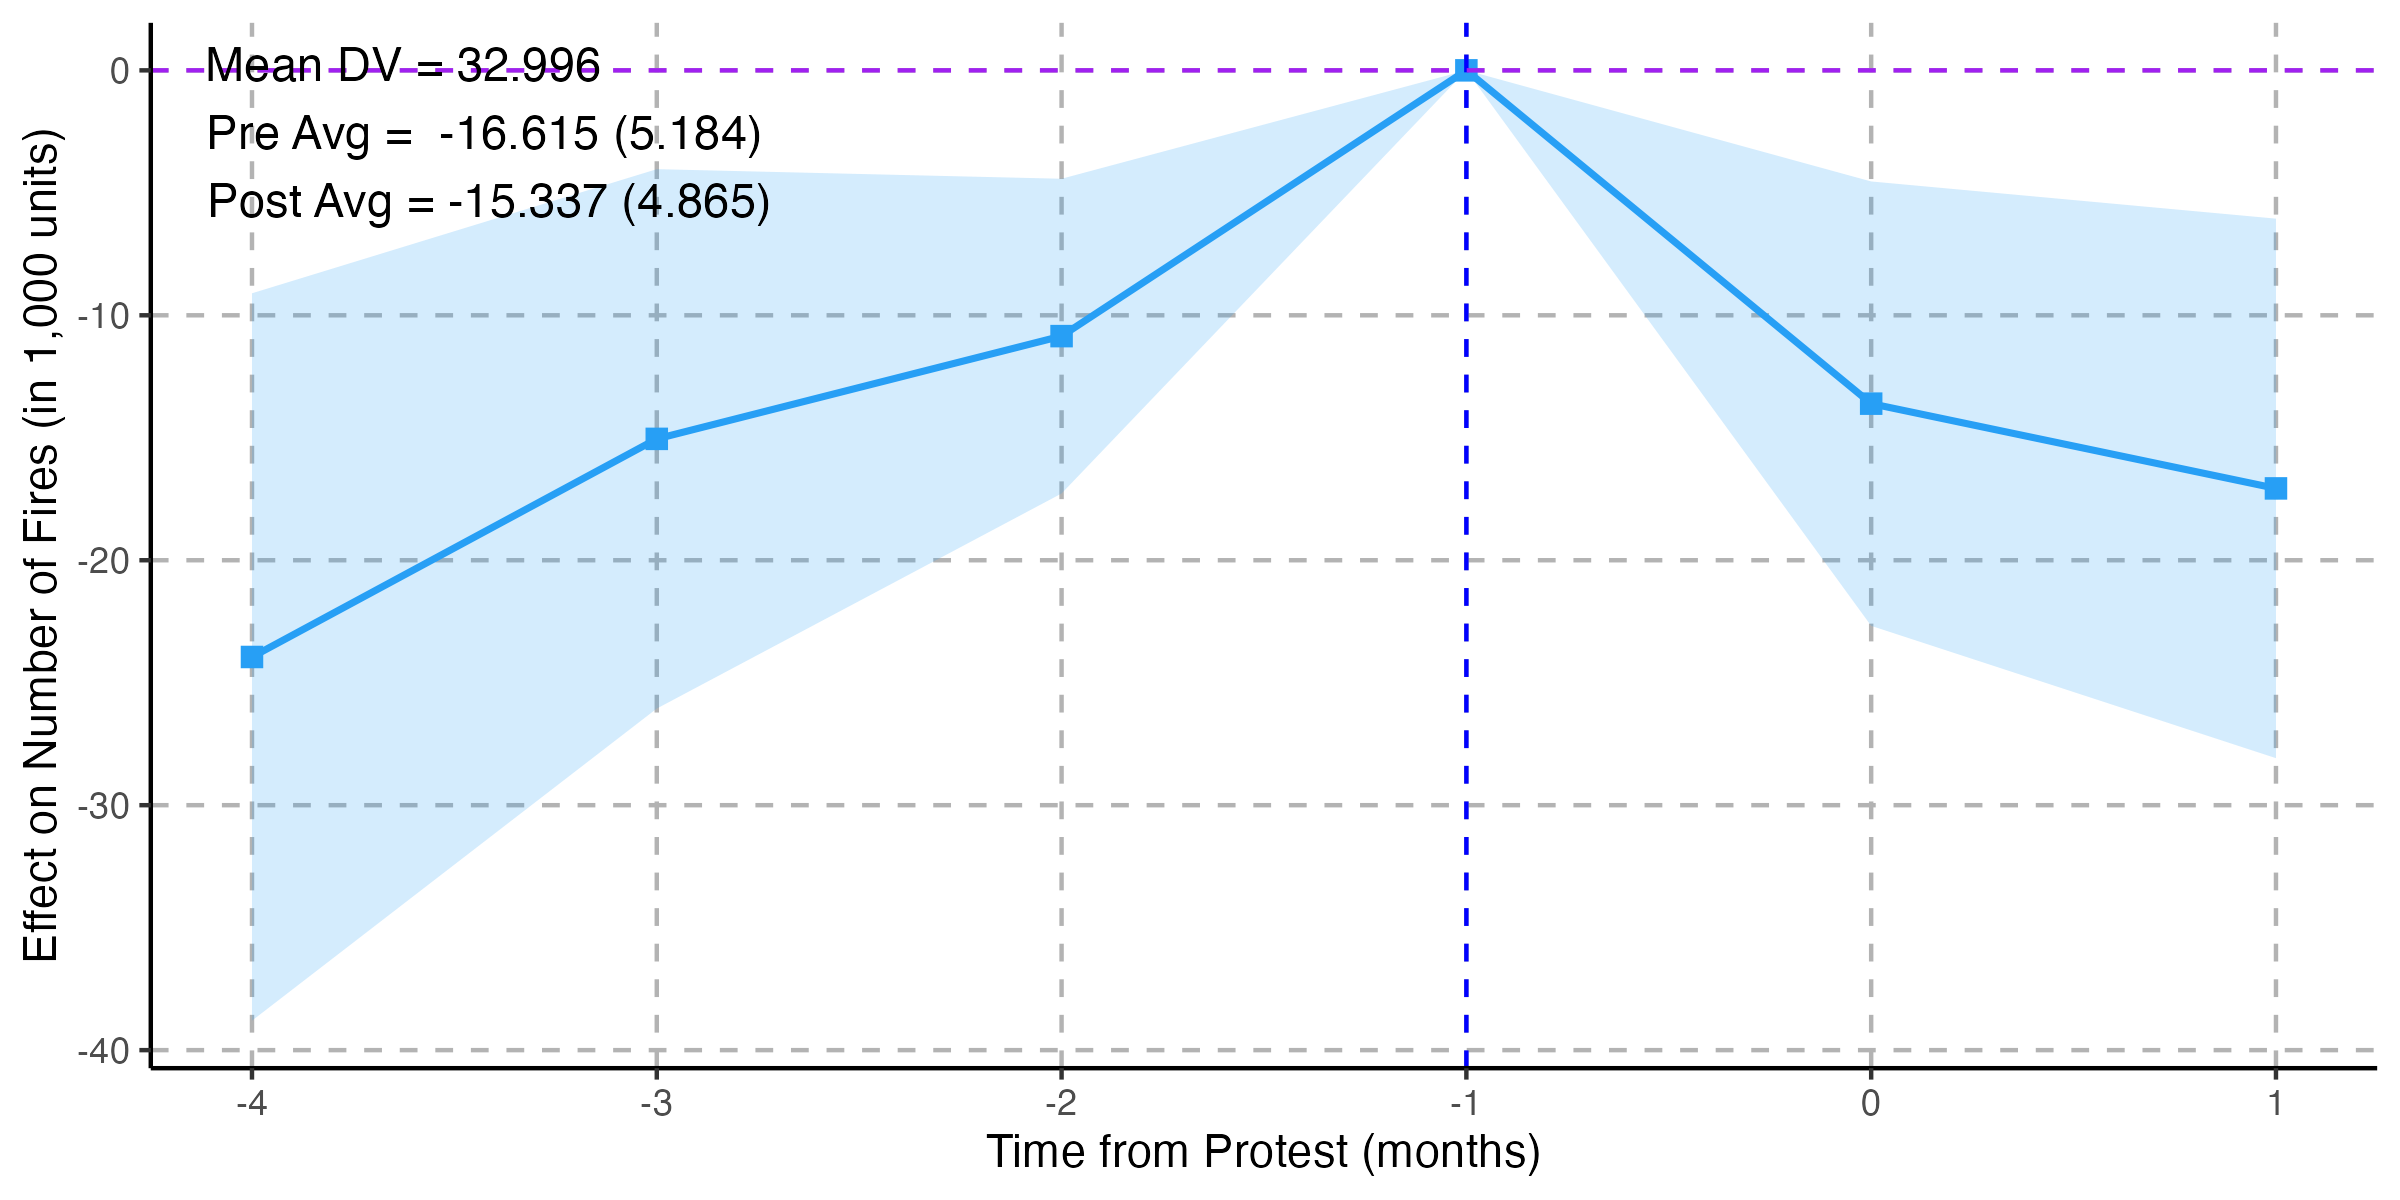
\includegraphics[width=0.85\linewidth]{../figures/app17_protest_evst_fe8_ori.png}
\caption{Event study, original (fe8)}
\end{figure}
\begin{figure}[H]
\centering
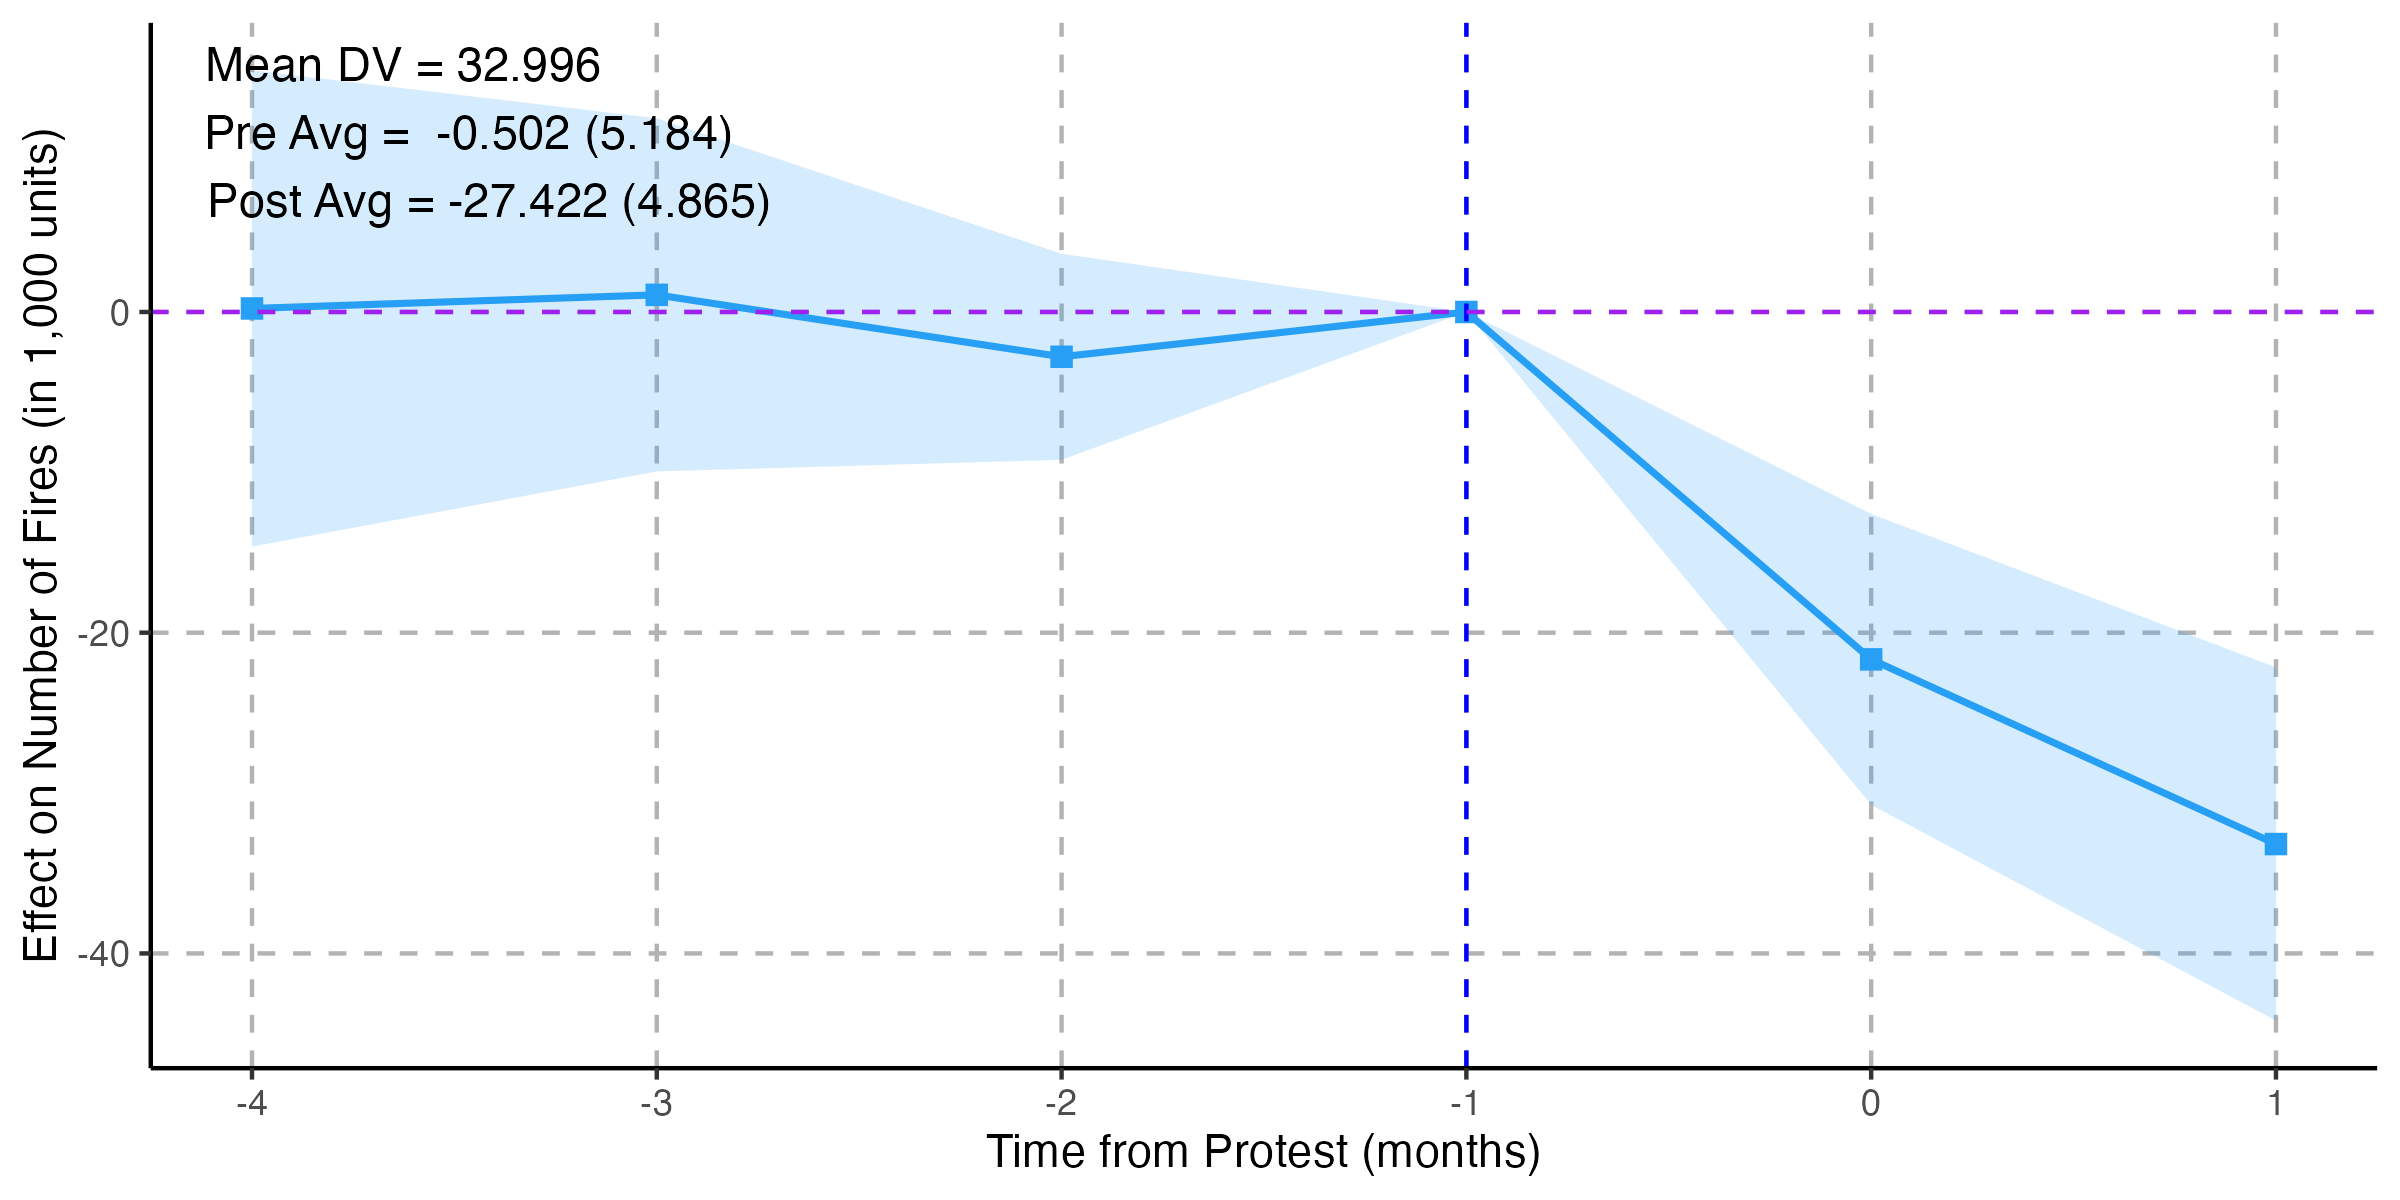
\includegraphics[width=0.85\linewidth]{../figures/app17_protest_evst_fe8_rotated.png}
\caption{Event study, linear-detrended (fe8)}
\end{figure}
\subsection*{FE specification \texttt{fe16} (slot `evreg3')}
\begin{figure}[H]
\centering
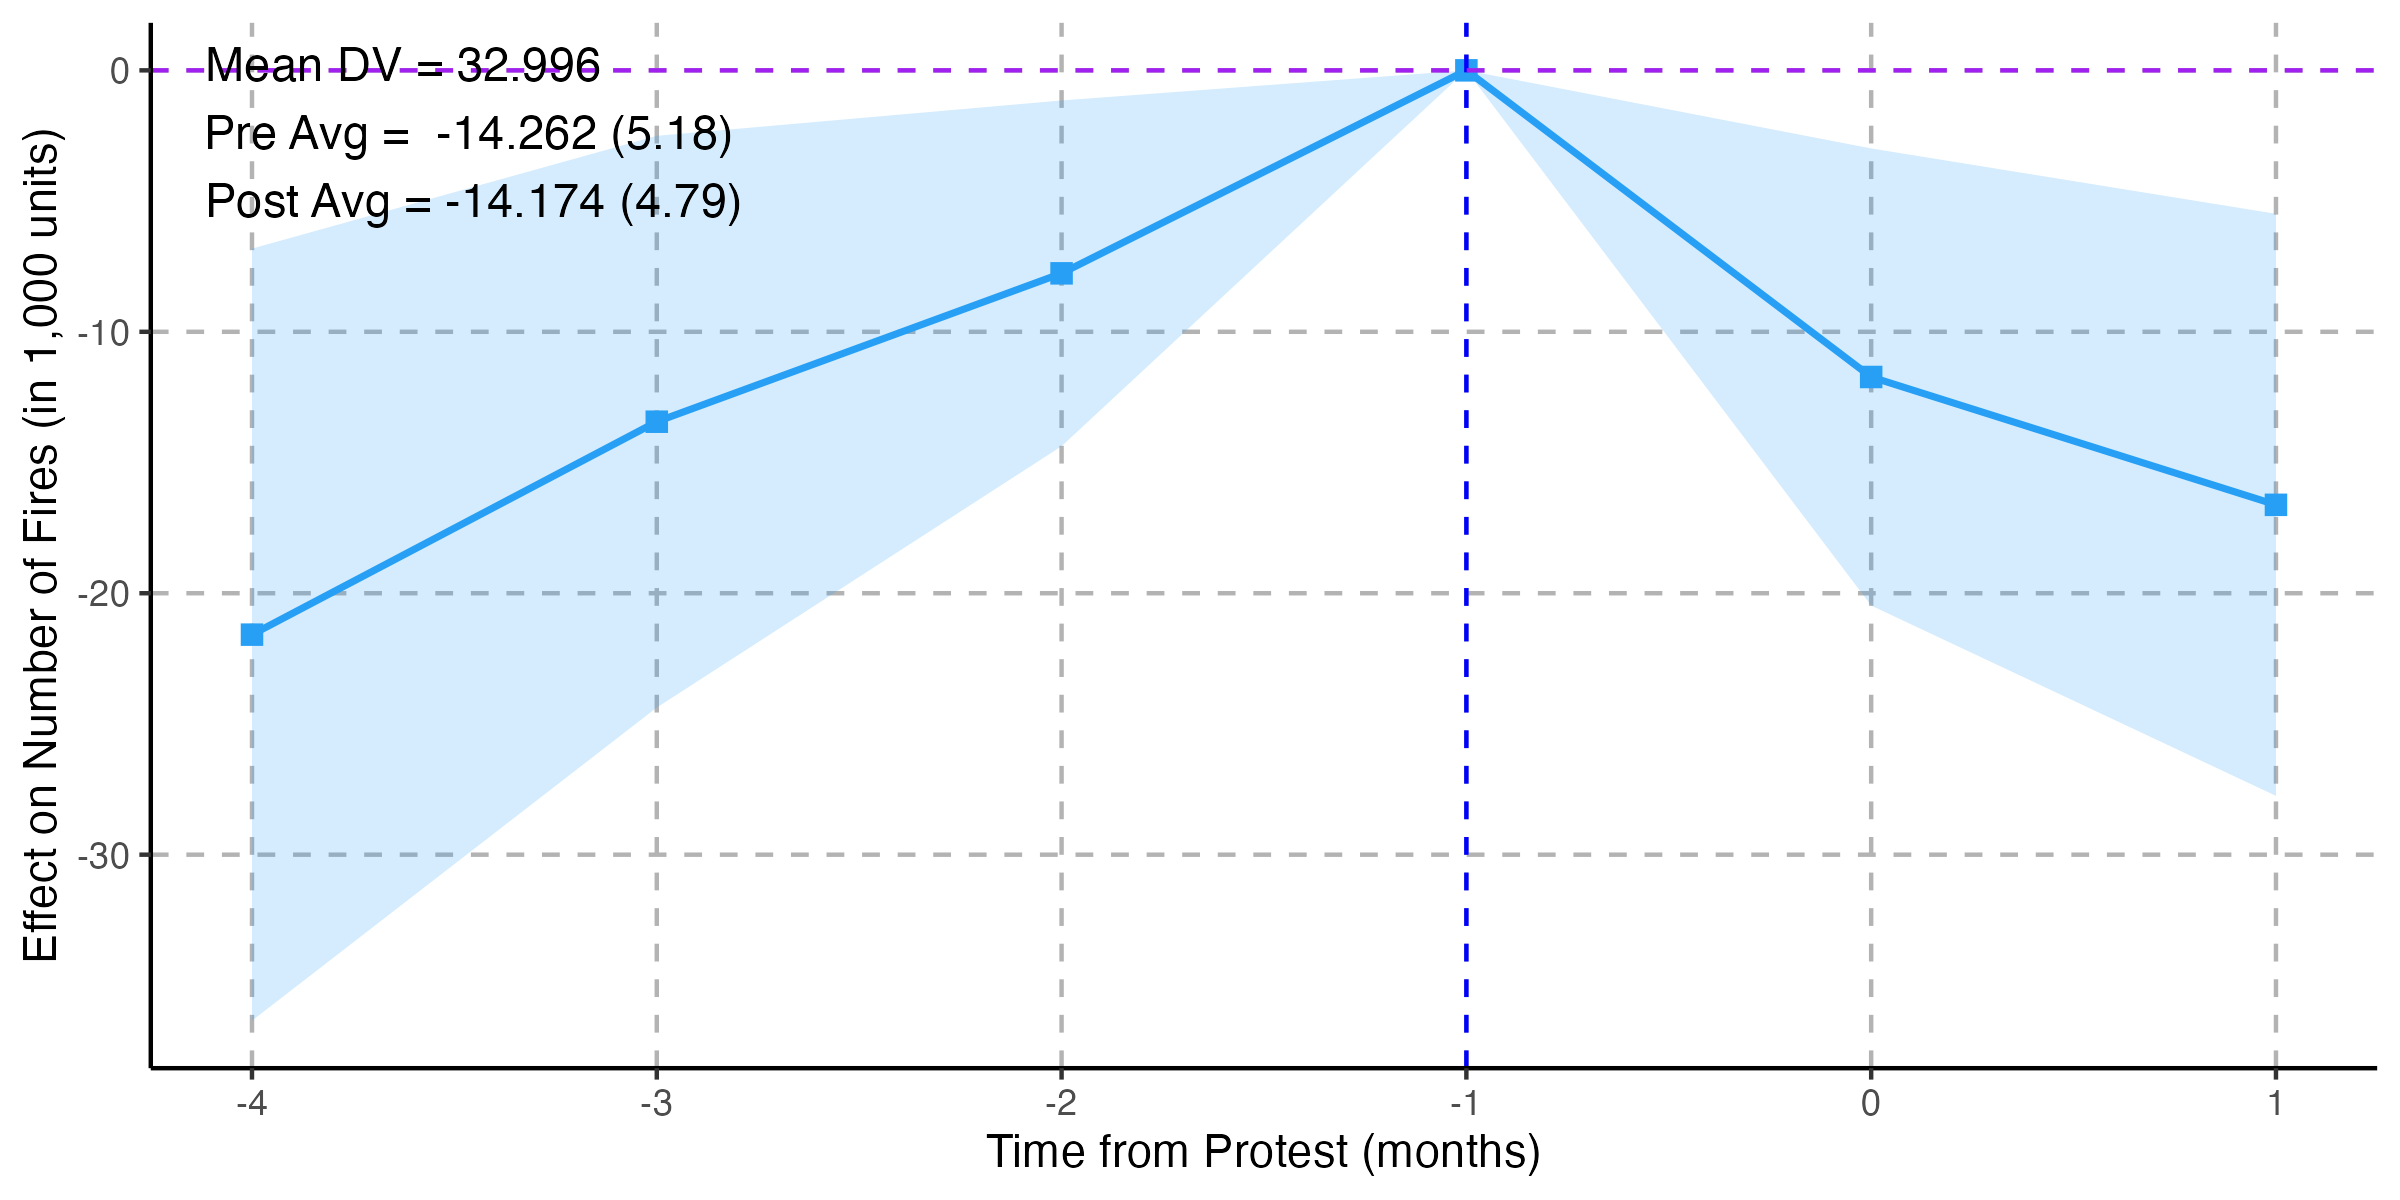
\includegraphics[width=0.85\linewidth]{../figures/app17_protest_evst_fe16_ori.png}
\caption{Event study, original (fe16)}
\end{figure}
\begin{figure}[H]
\centering
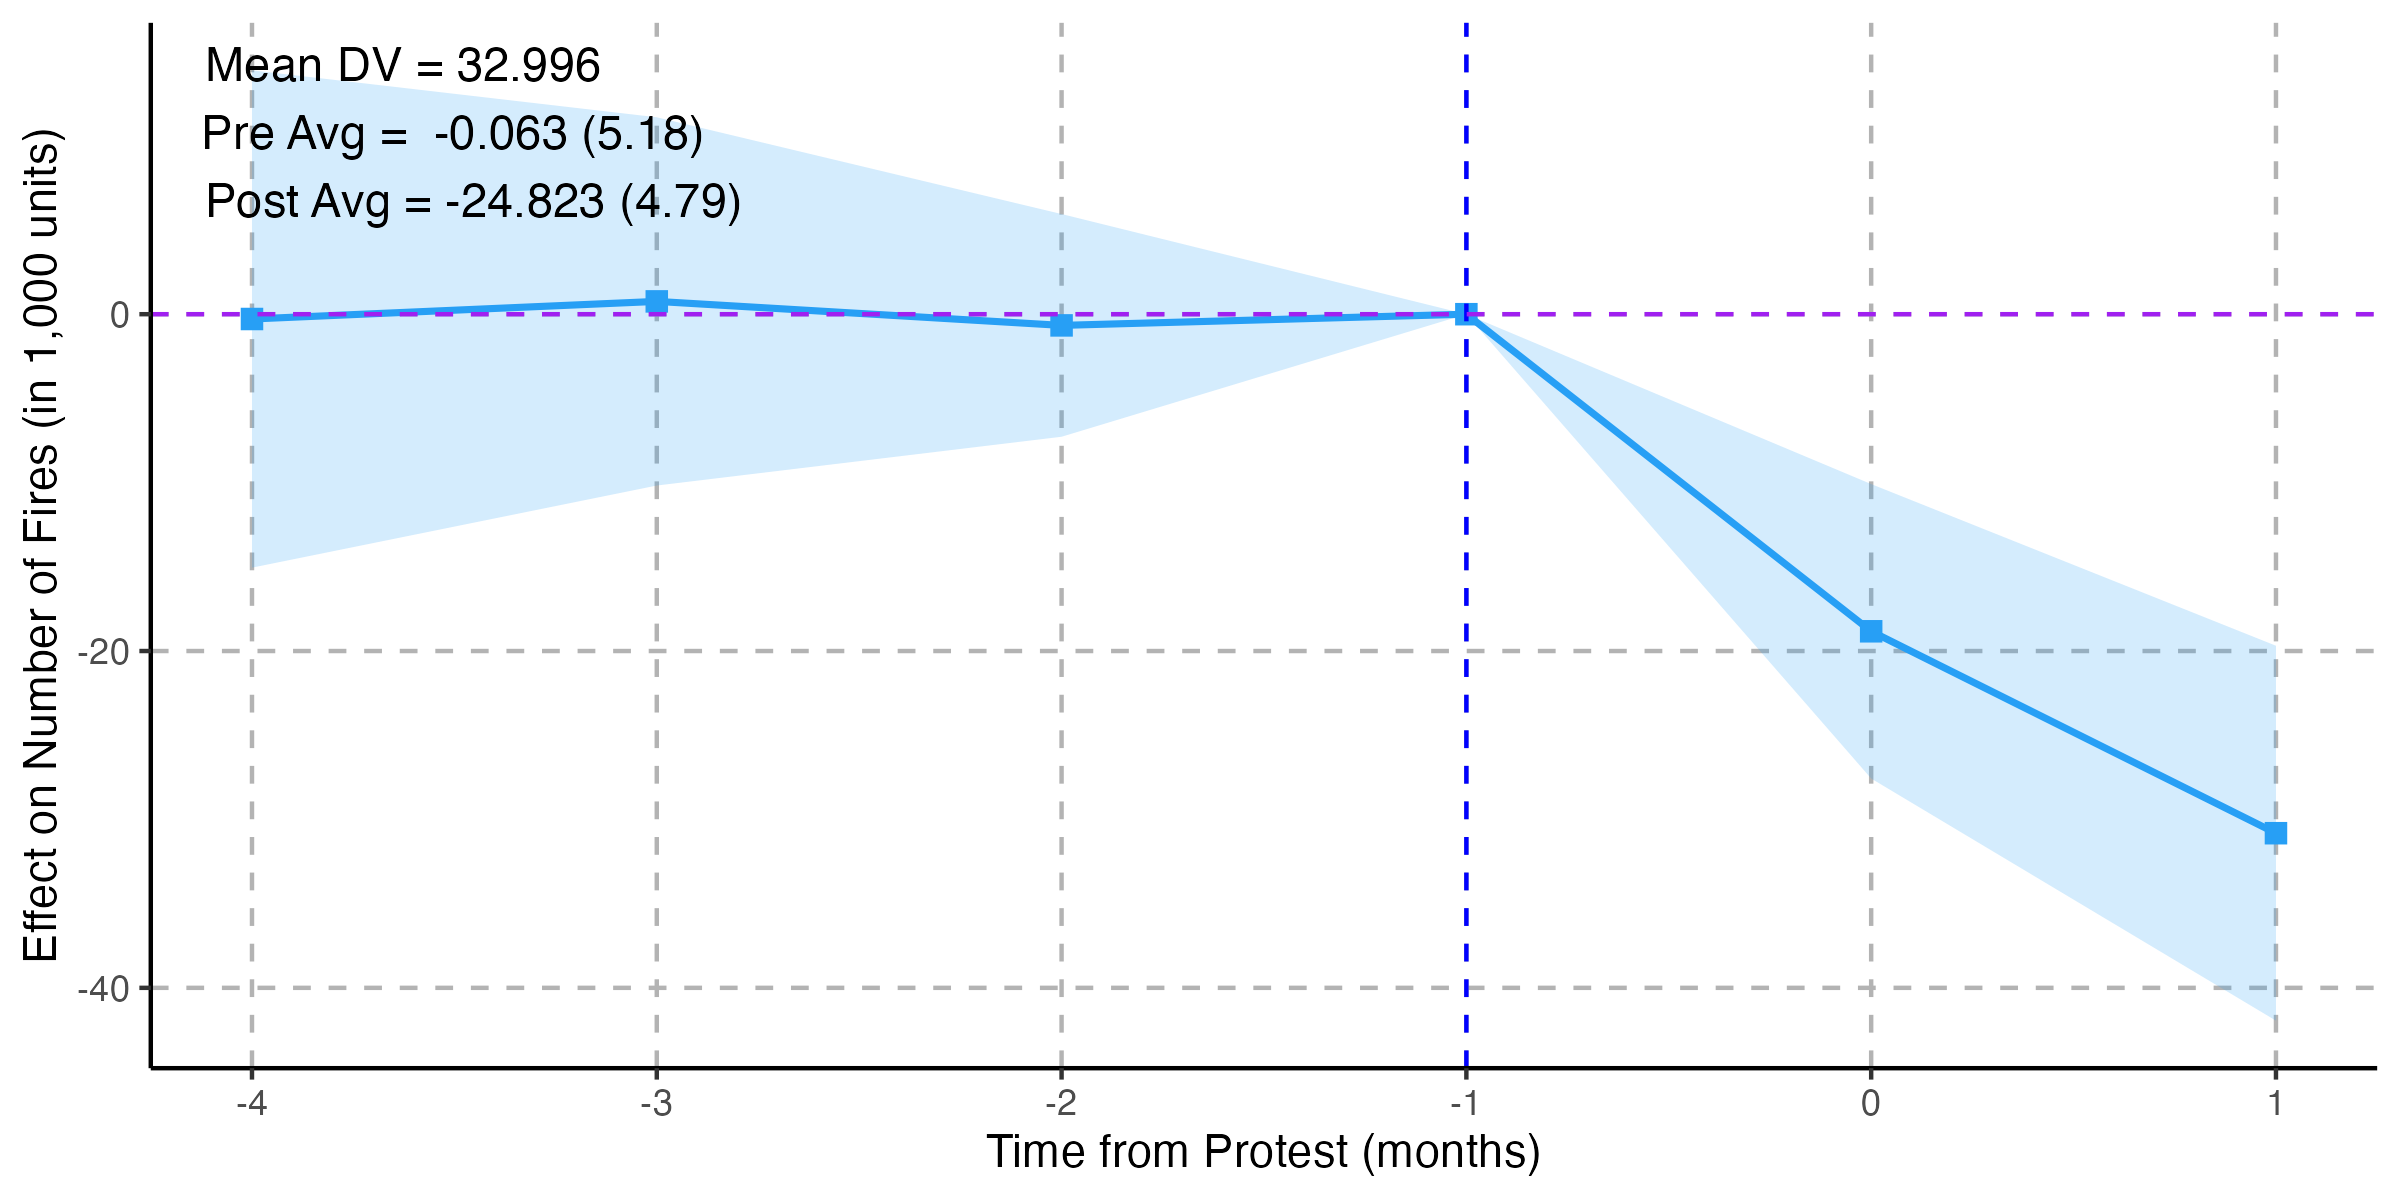
\includegraphics[width=0.85\linewidth]{../figures/app17_protest_evst_fe16_rotated.png}
\caption{Event study, linear-detrended (fe16)}
\end{figure}
\subsection*{FE specification \texttt{fe24} (slot `evreg4')}
\begin{figure}[H]
\centering
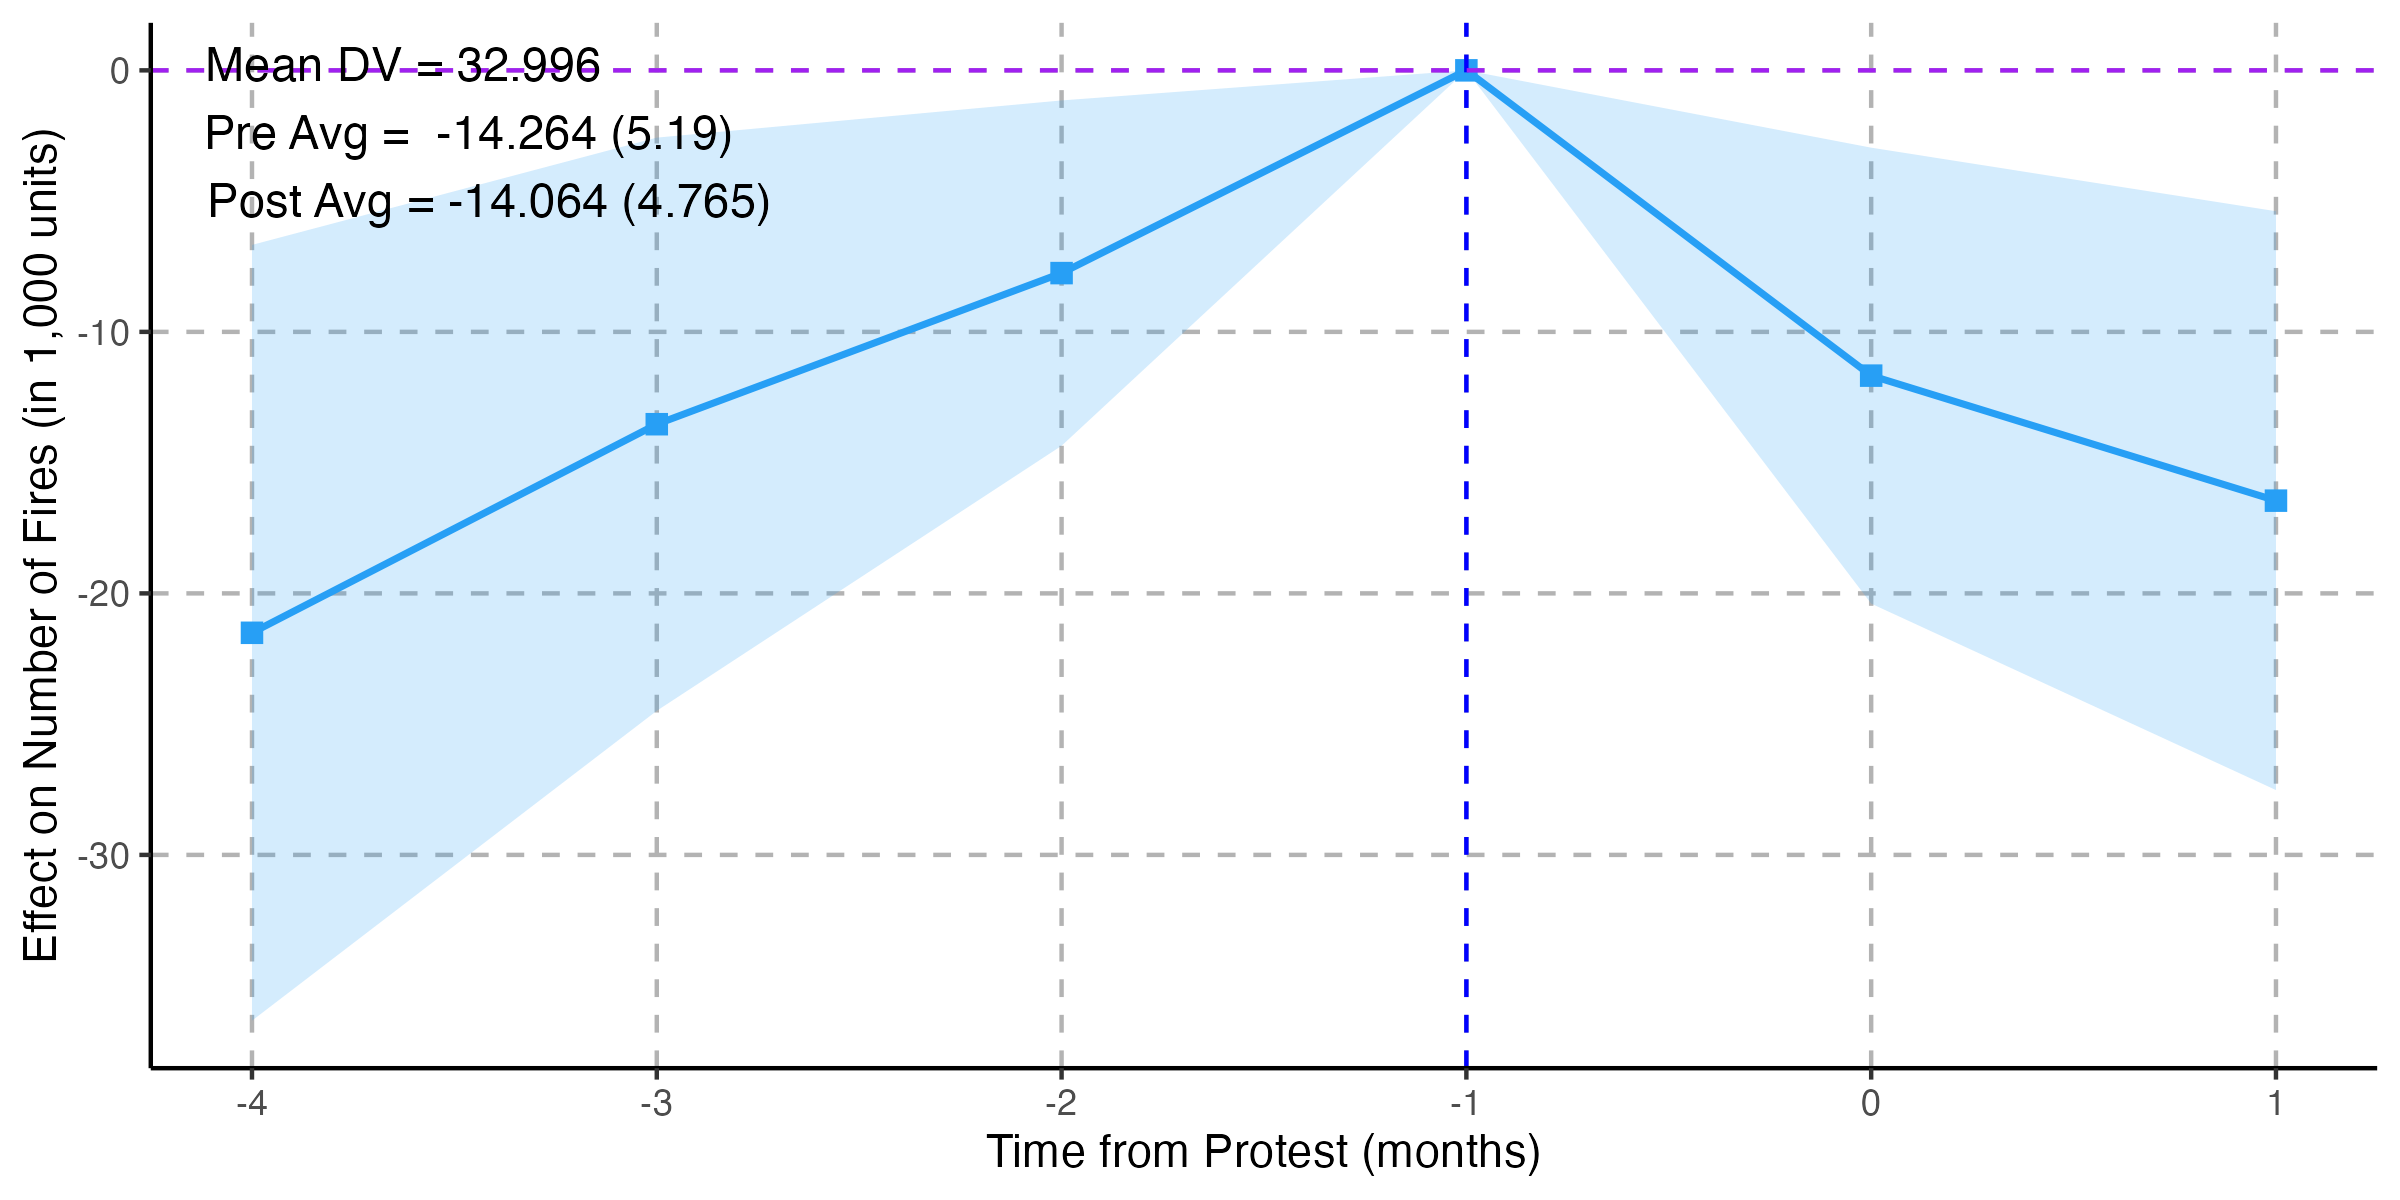
\includegraphics[width=0.85\linewidth]{../figures/app17_protest_evst_fe24_ori.png}
\caption{Event study, original (fe24)}
\end{figure}
\begin{figure}[H]
\centering
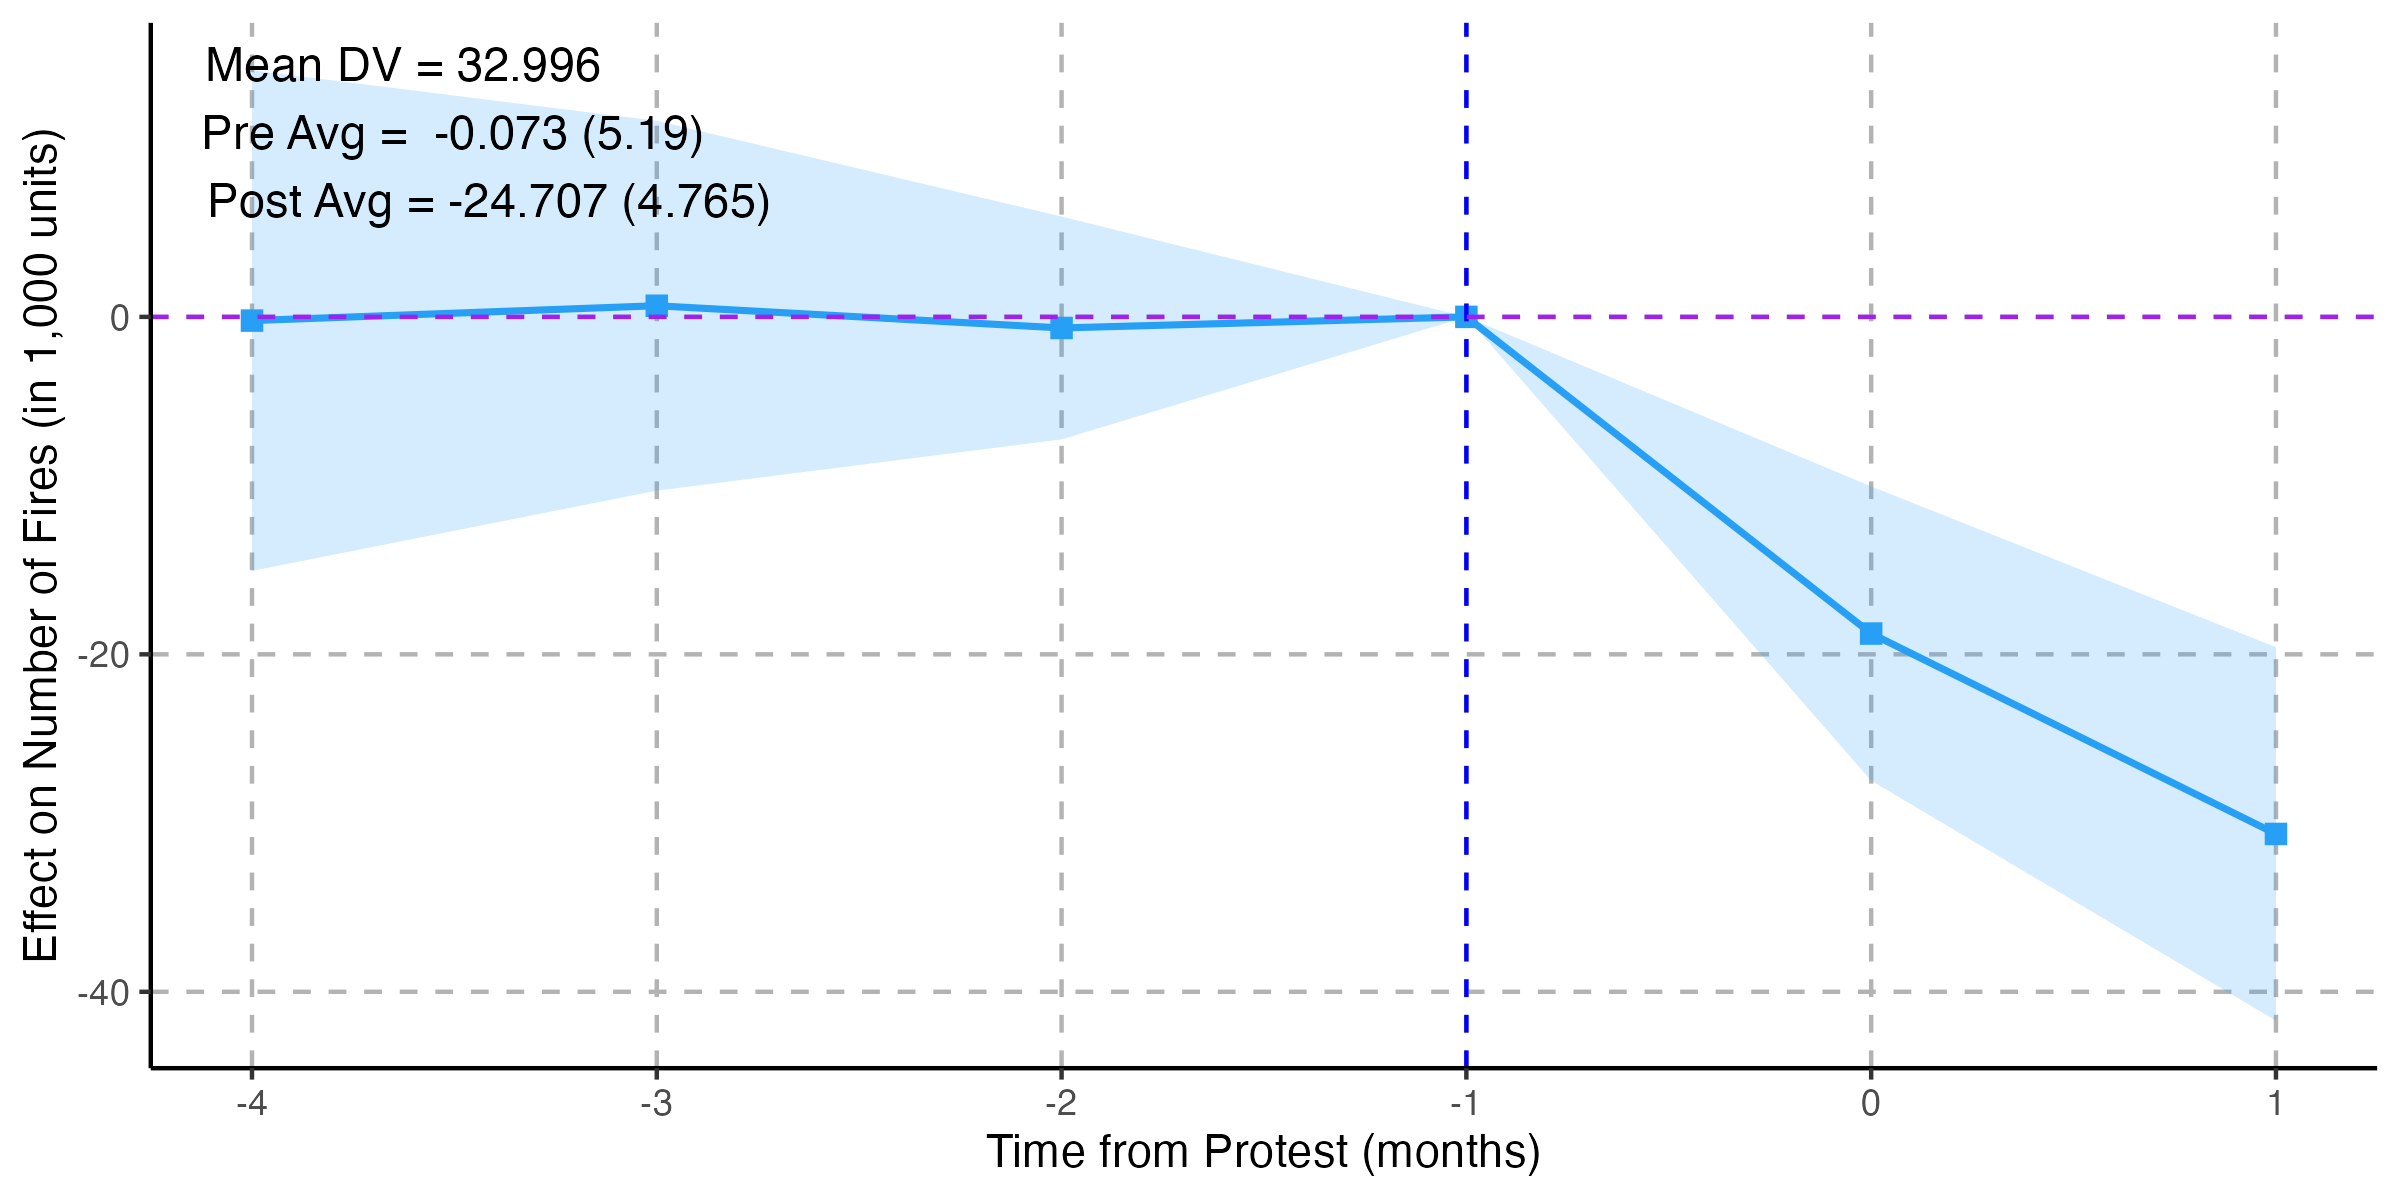
\includegraphics[width=0.85\linewidth]{../figures/app17_protest_evst_fe24_rotated.png}
\caption{Event study, linear-detrended (fe24)}
\end{figure}
\subsection*{FE specification \texttt{fe32} (slot `evreg5')}
\begin{figure}[H]
\centering
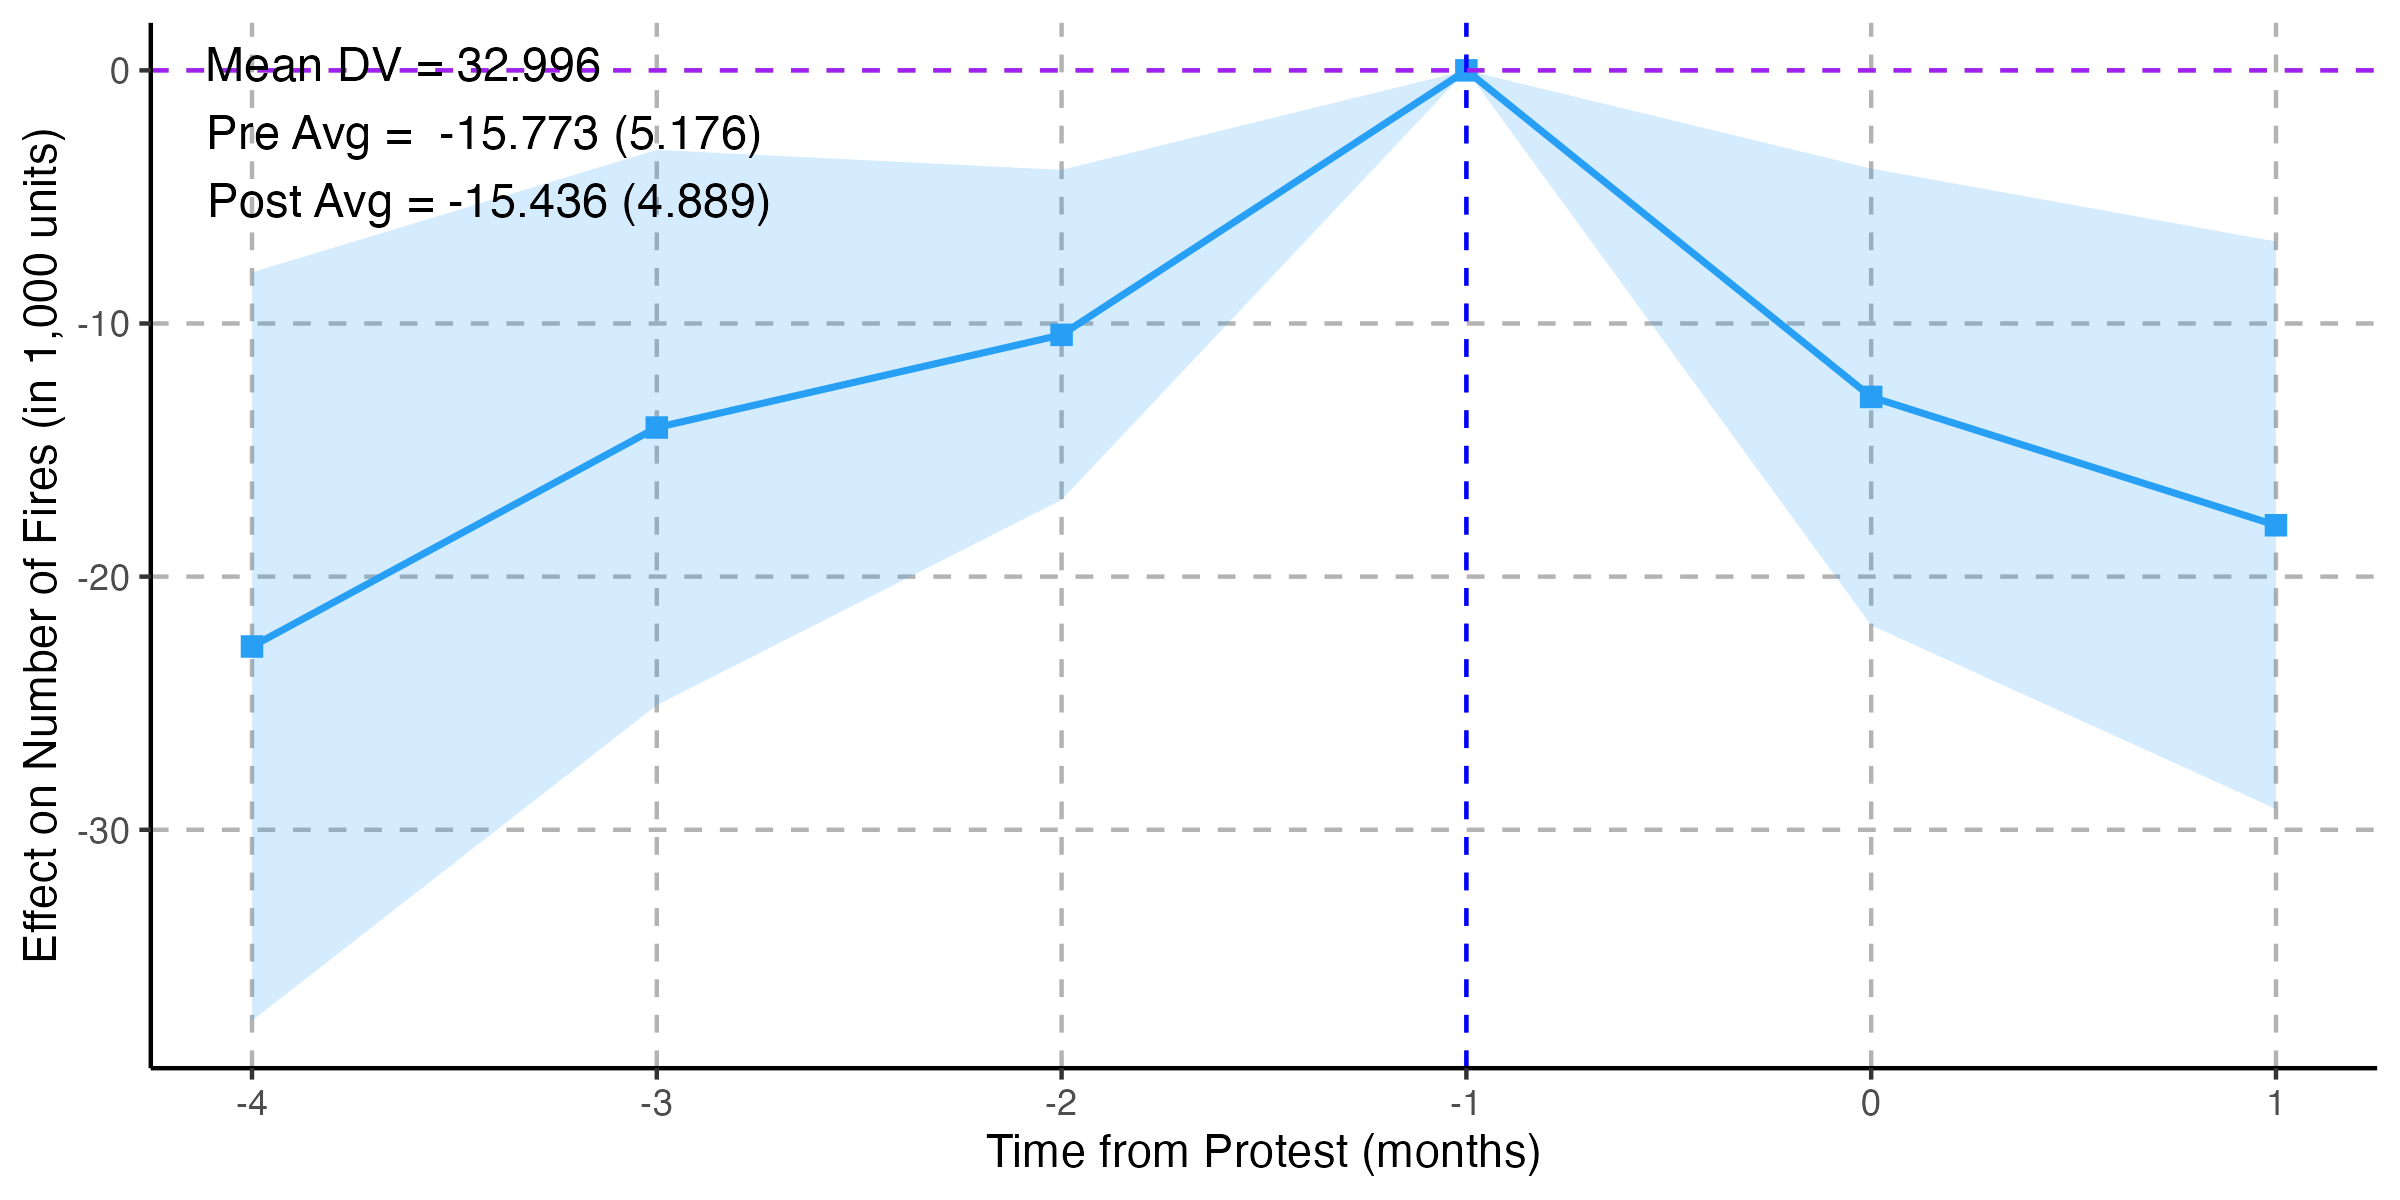
\includegraphics[width=0.85\linewidth]{../figures/app17_protest_evst_fe32_ori.png}
\caption{Event study, original (fe32)}
\end{figure}
\begin{figure}[H]
\centering
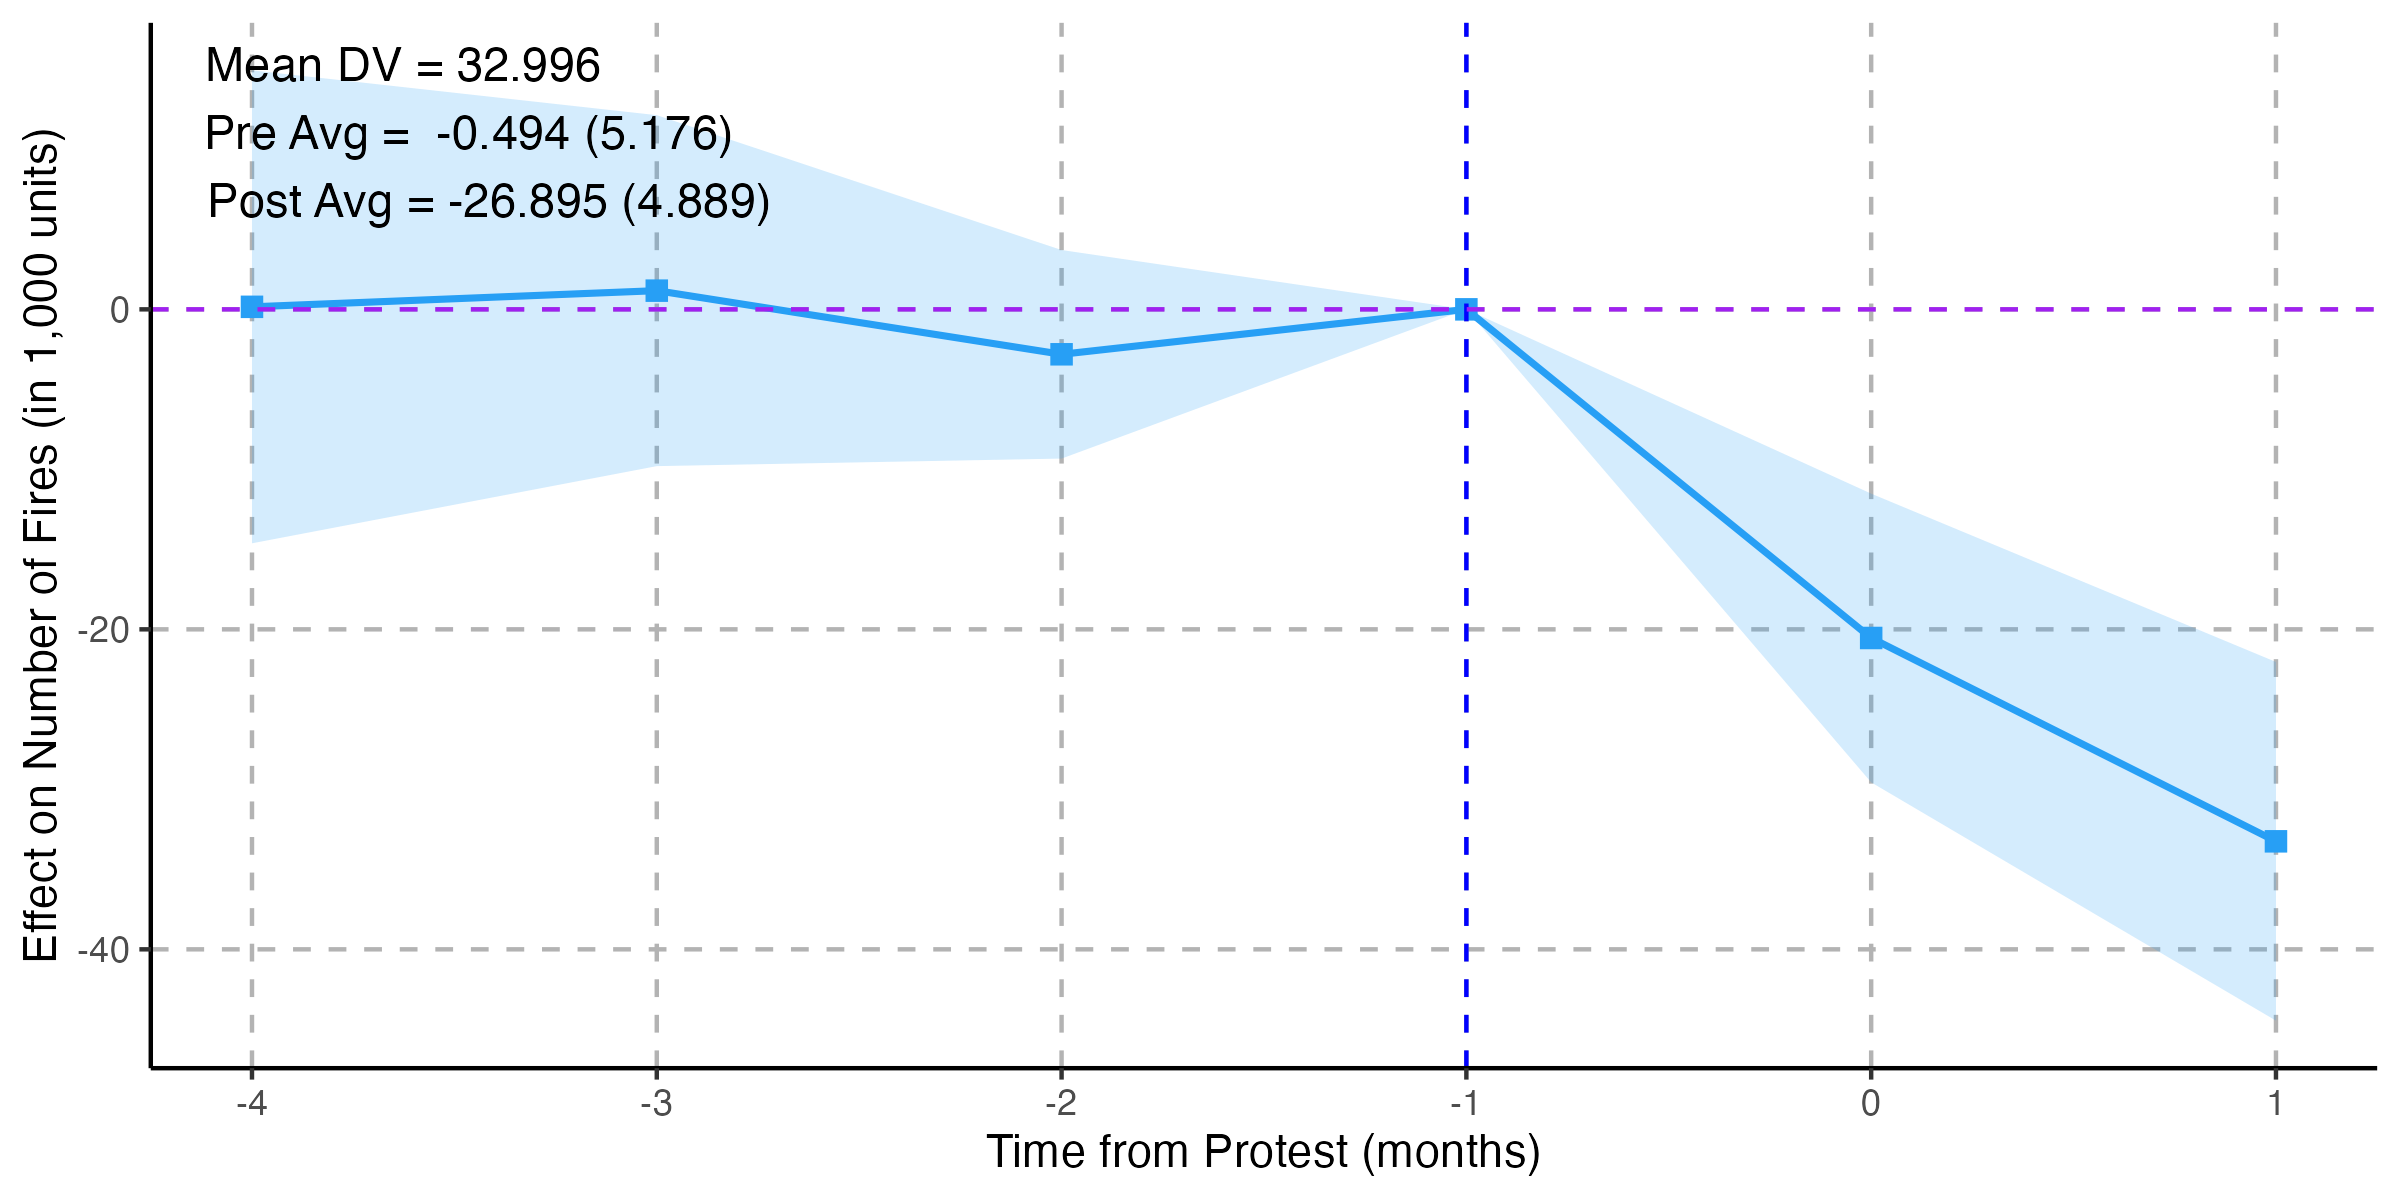
\includegraphics[width=0.85\linewidth]{../figures/app17_protest_evst_fe32_rotated.png}
\caption{Event study, linear-detrended (fe32)}
\end{figure}
\FloatBarrier
\clearpage
\section{Interaction DiD --- Protest with \texttt{downup\_ac} (\texttt{\_app\_18})}
\subsection*{FE specification \texttt{fe1} (slot `evreg1')}
\begin{figure}[H]
\centering
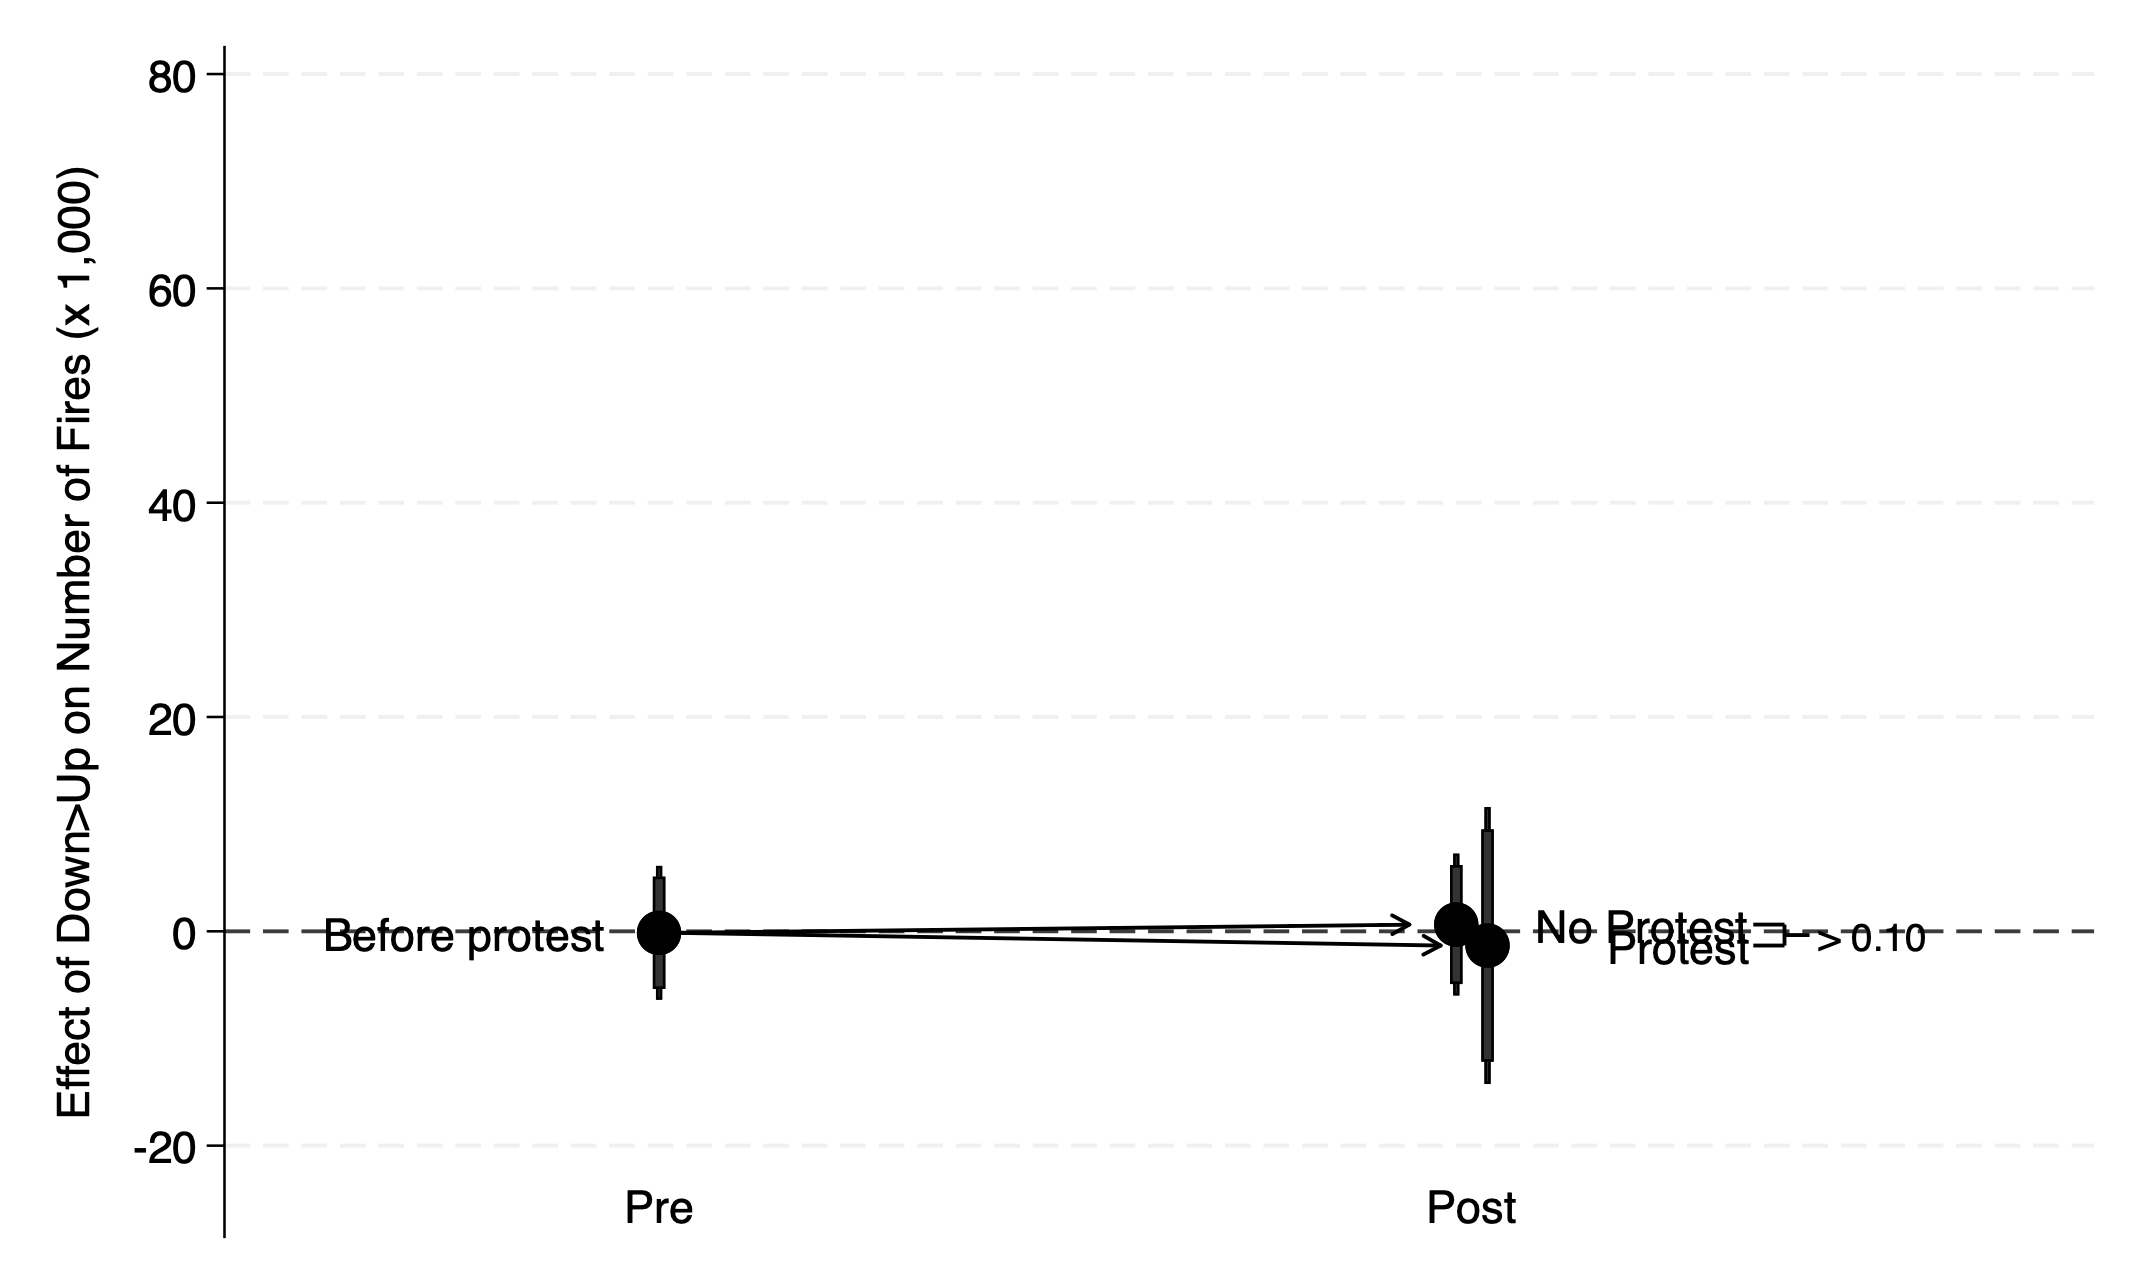
\includegraphics[width=0.85\linewidth]{../figures/app18_protest_did_downup_1.png}
\caption{Protest $\times$ downup\_ac (fe1)}
\end{figure}
\subsection*{FE specification \texttt{fe8} (slot `evreg2')}
\begin{figure}[H]
\centering
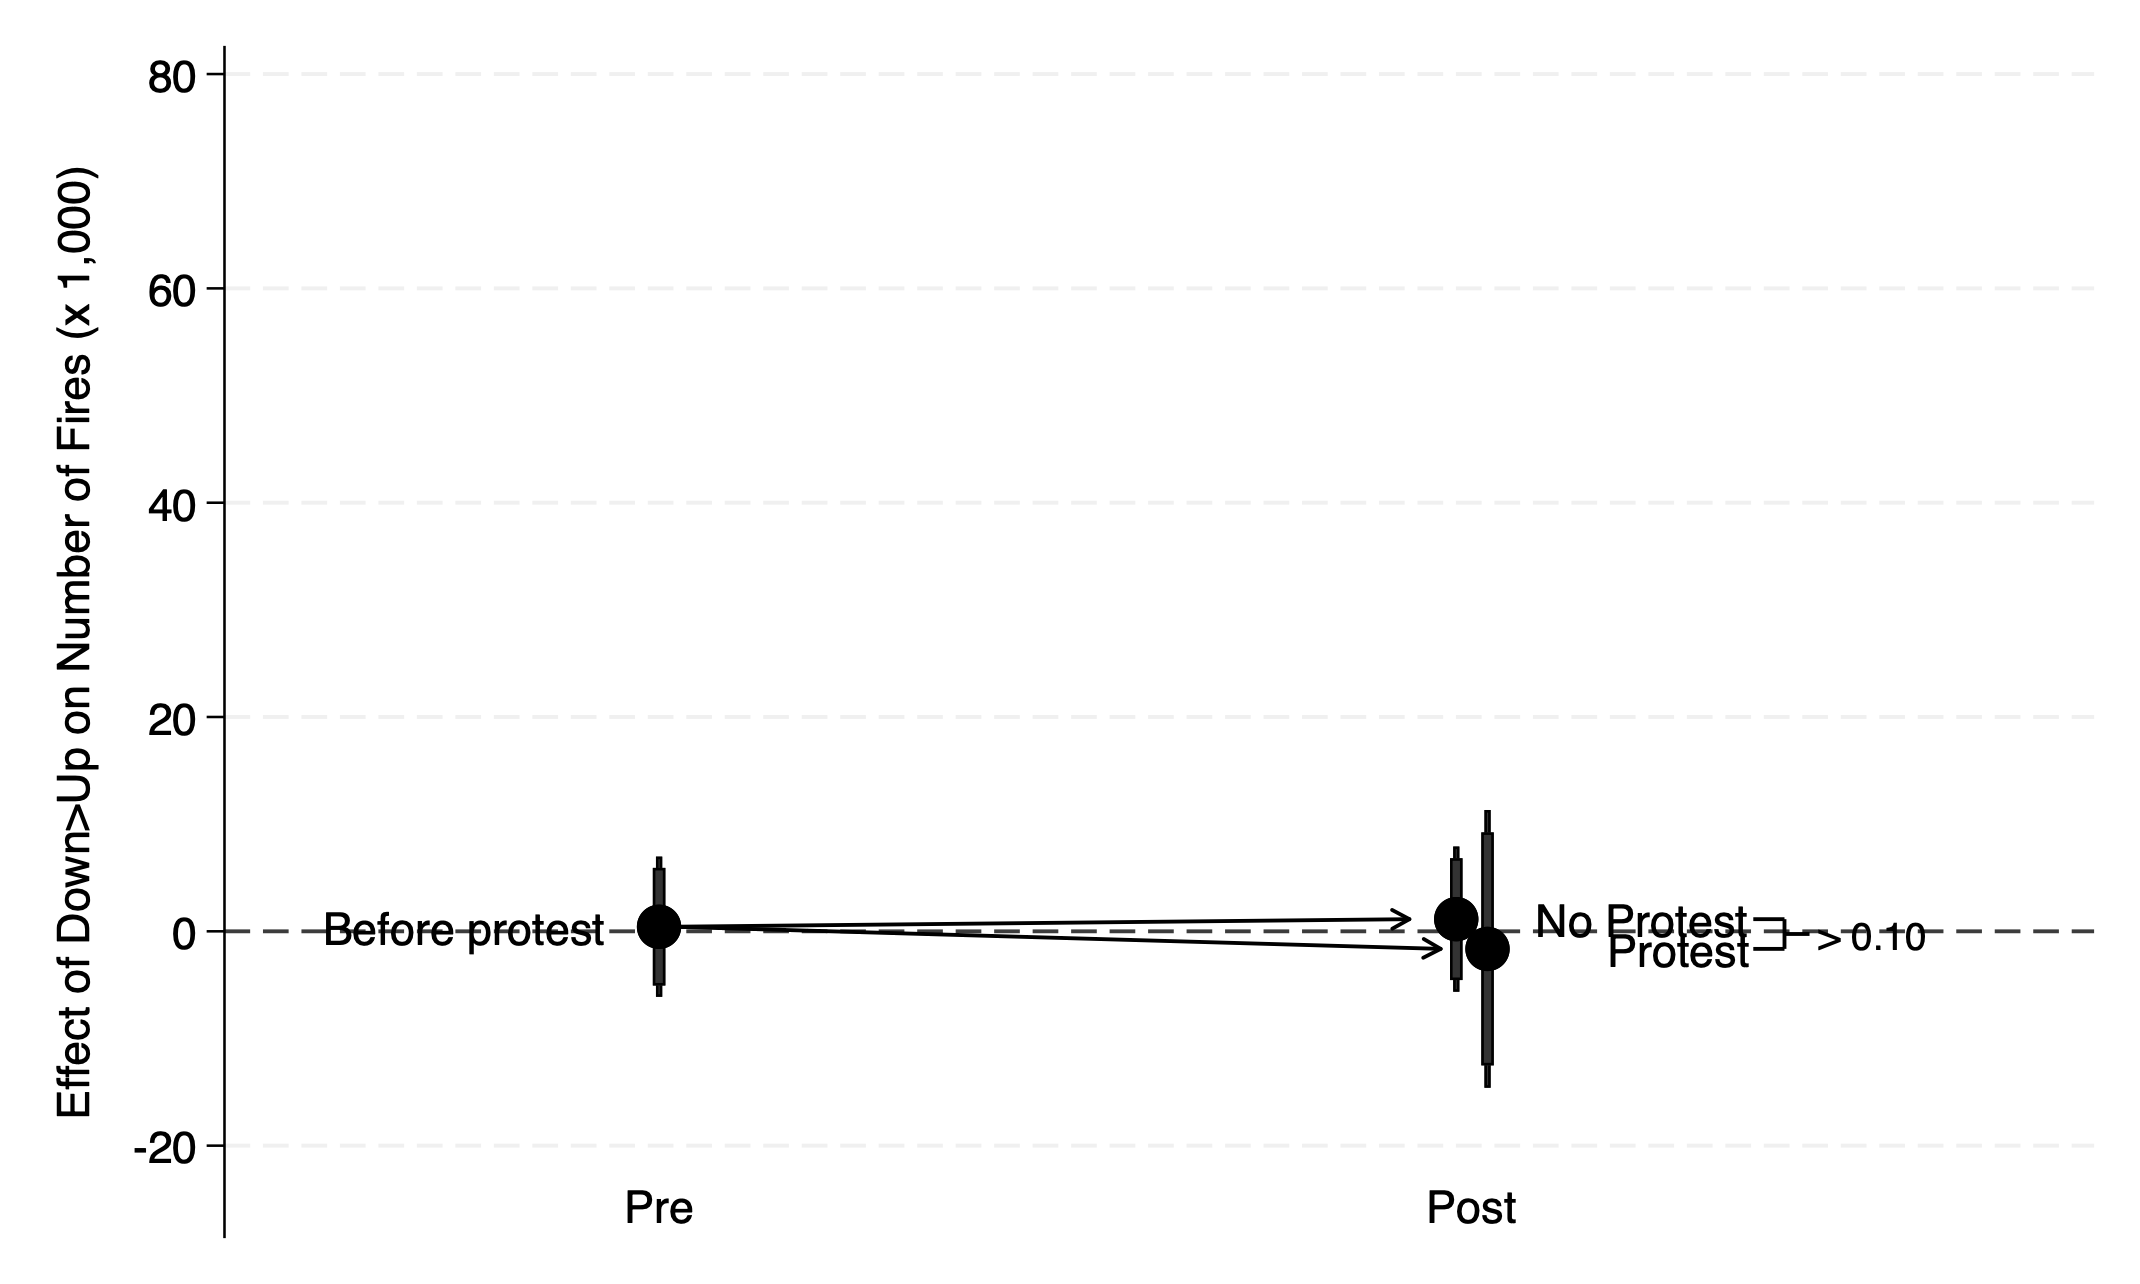
\includegraphics[width=0.85\linewidth]{../figures/app18_protest_did_downup_2.png}
\caption{Protest $\times$ downup\_ac (fe8)}
\end{figure}
\subsection*{FE specification \texttt{fe16} (slot `evreg3')}
\begin{figure}[H]
\centering
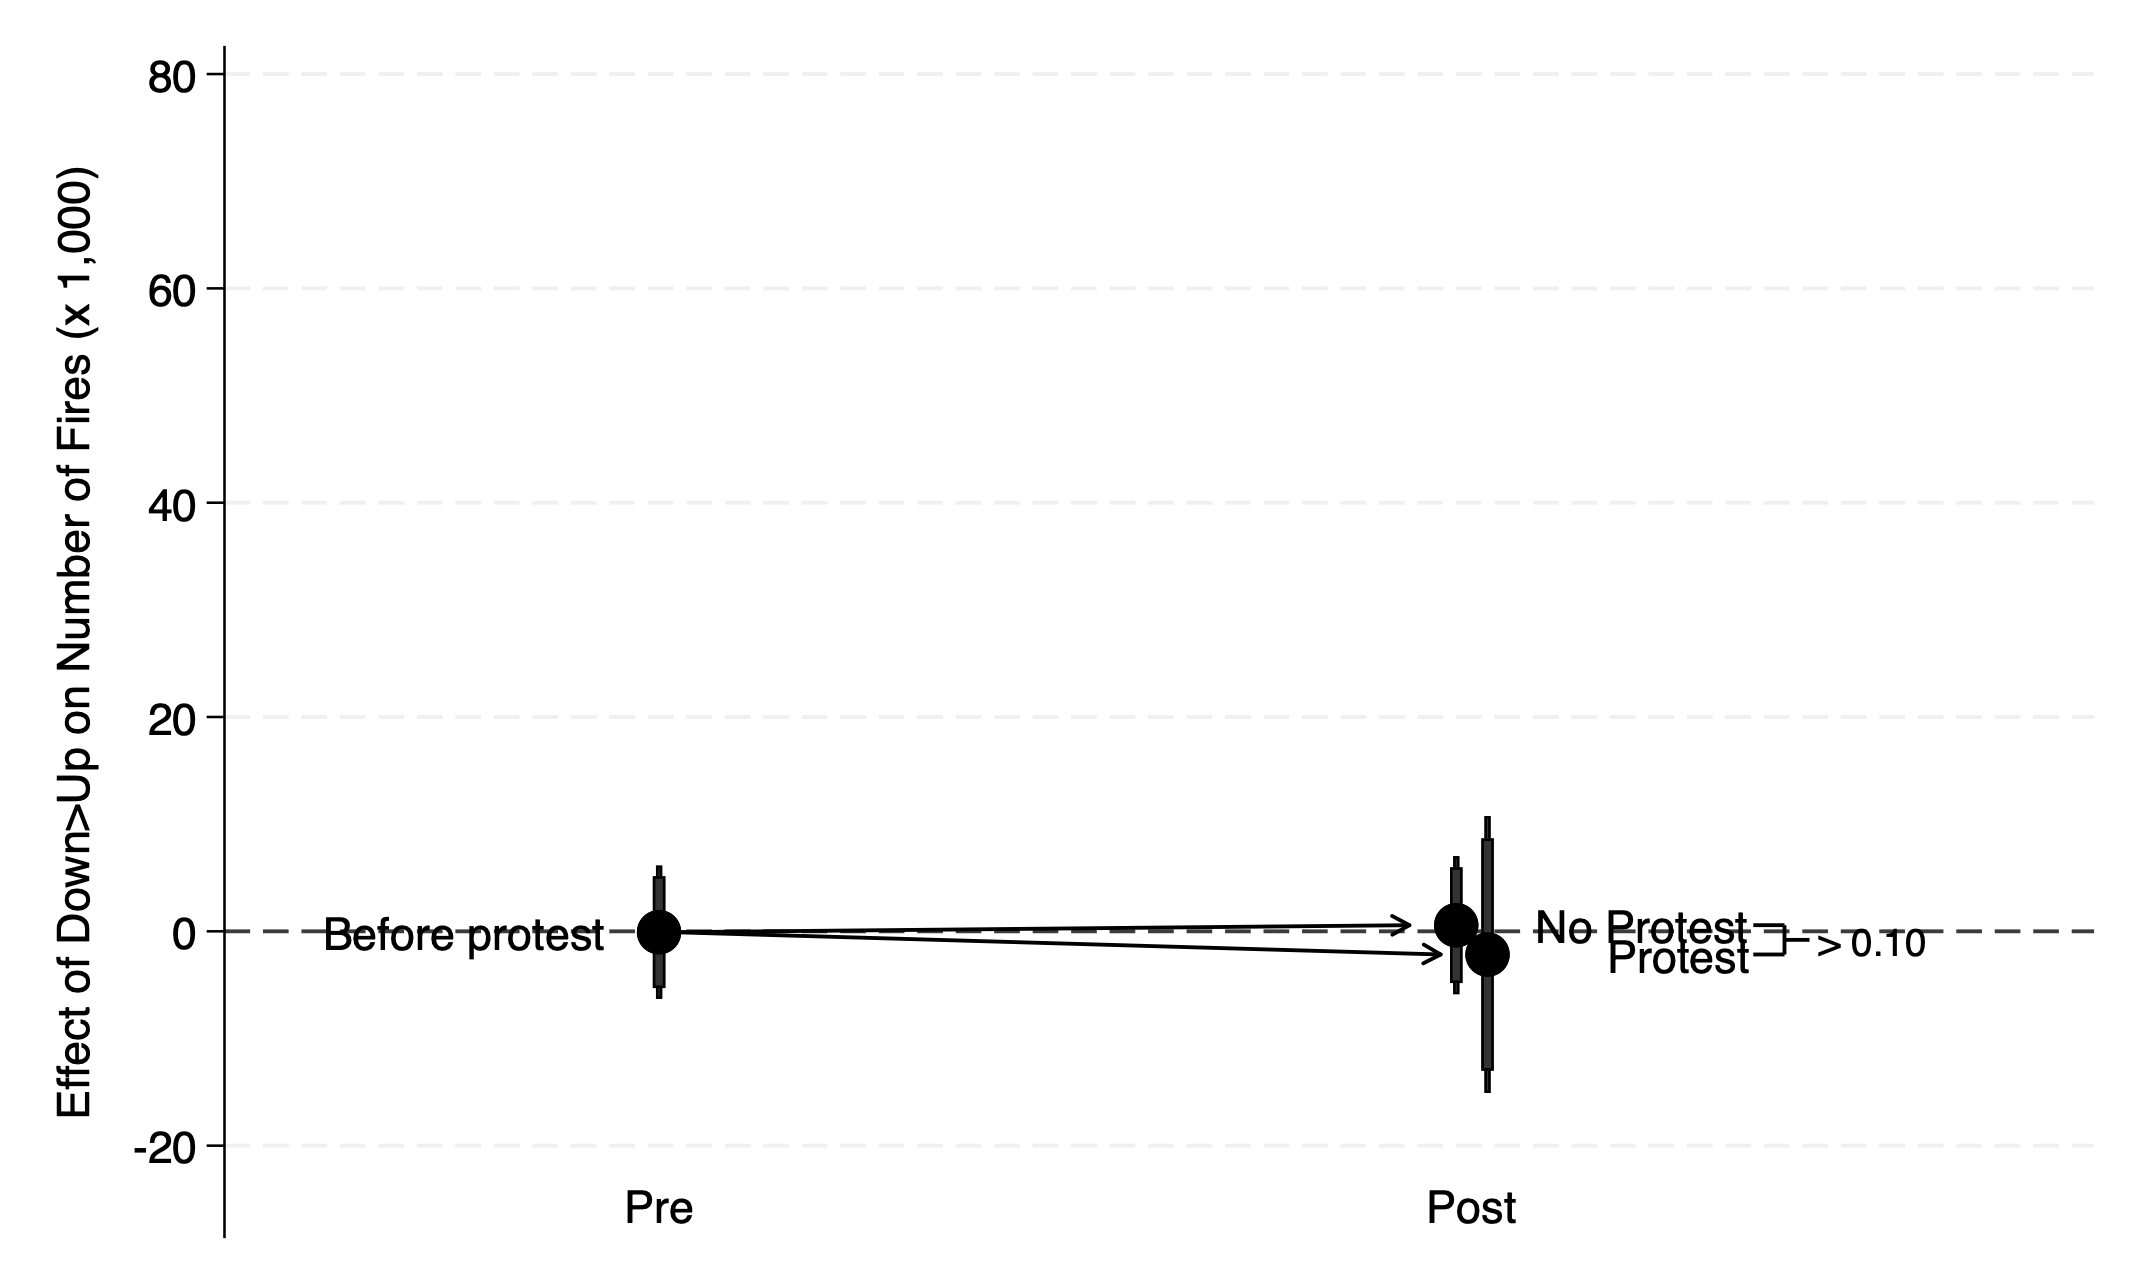
\includegraphics[width=0.85\linewidth]{../figures/app18_protest_did_downup_3.png}
\caption{Protest $\times$ downup\_ac (fe16)}
\end{figure}
\subsection*{FE specification \texttt{fe24} (slot `evreg4')}
\begin{figure}[H]
\centering
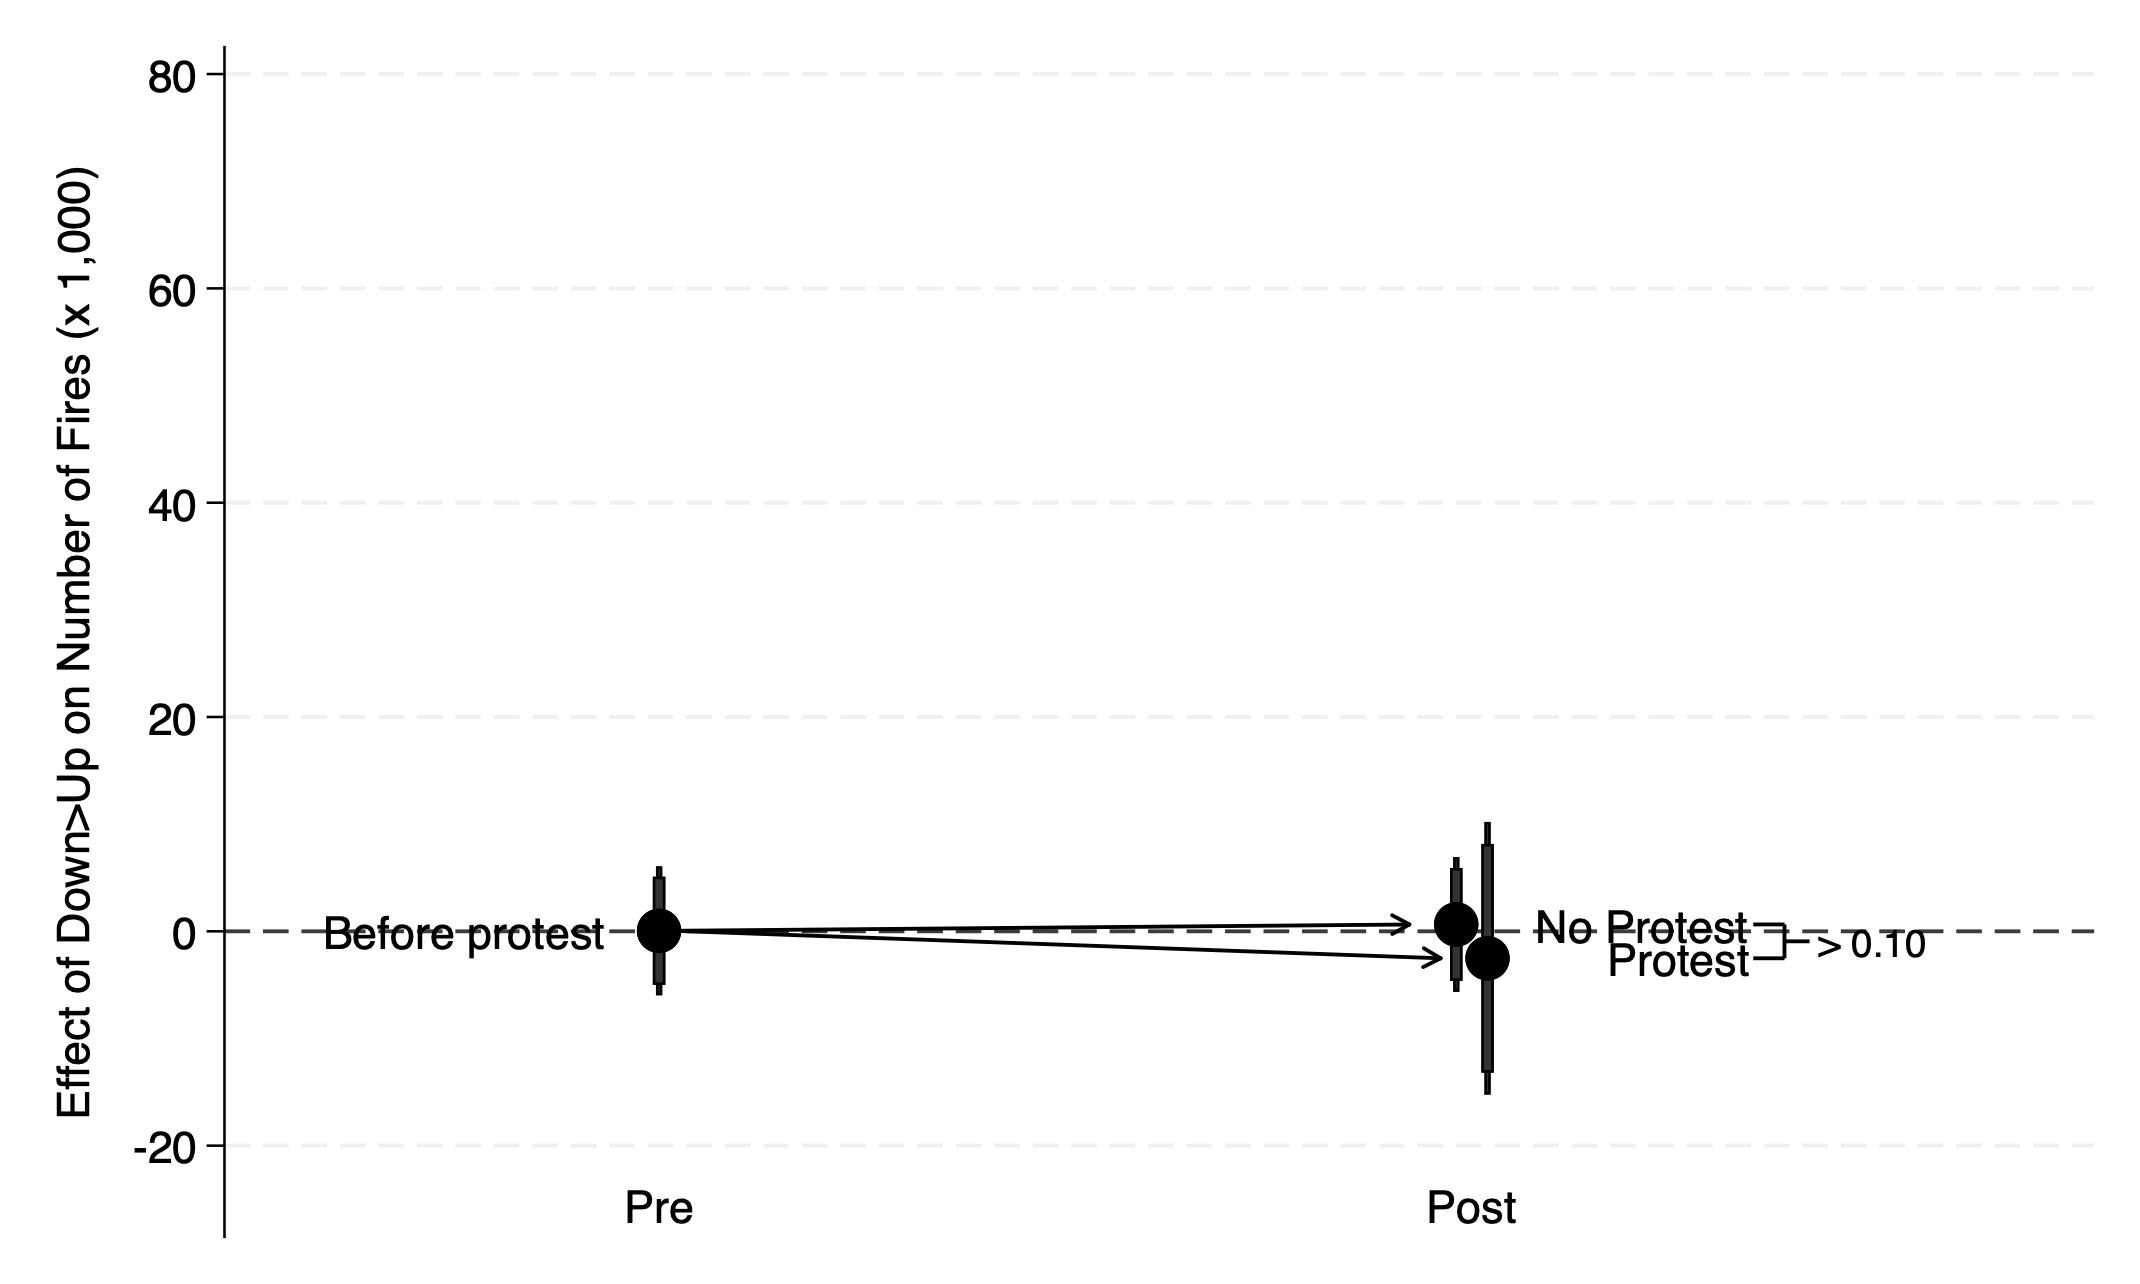
\includegraphics[width=0.85\linewidth]{../figures/app18_protest_did_downup_4.png}
\caption{Protest $\times$ downup\_ac (fe24)}
\end{figure}
\subsection*{FE specification \texttt{fe32} (slot `evreg5')}
\begin{figure}[H]
\centering
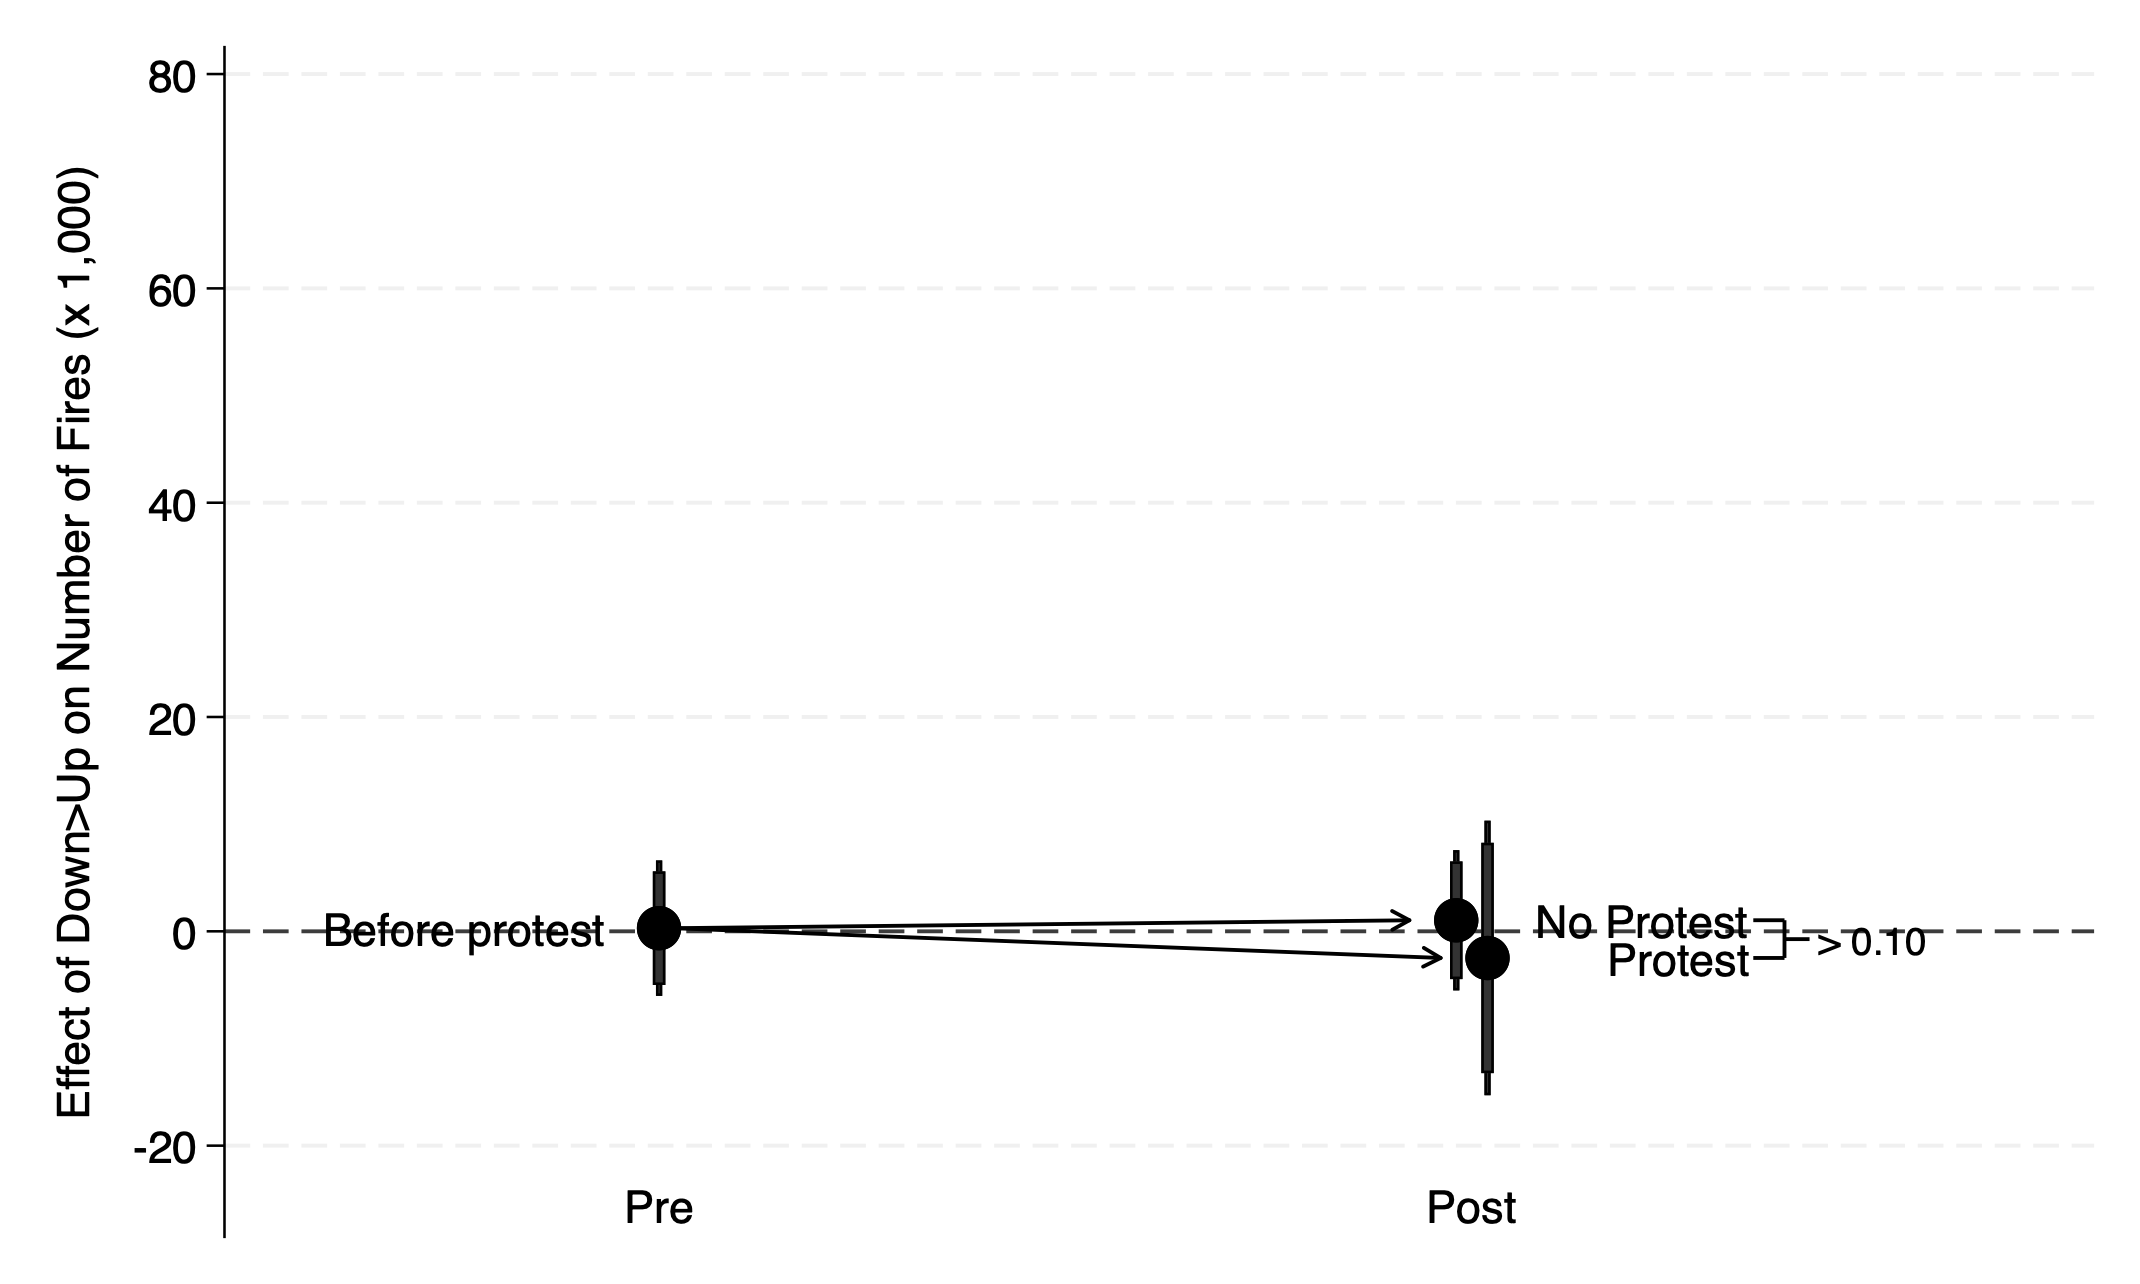
\includegraphics[width=0.85\linewidth]{../figures/app18_protest_did_downup_5.png}
\caption{Protest $\times$ downup\_ac (fe32)}
\end{figure}
\FloatBarrier
\clearpage
\section{Interaction DiD --- Politician characteristics with \texttt{downup\_ac} (\texttt{\_app\_19})}
\subsection*{FE specification \texttt{fe1} (slot `evreg1')}
\begin{figure}[H]
\centering
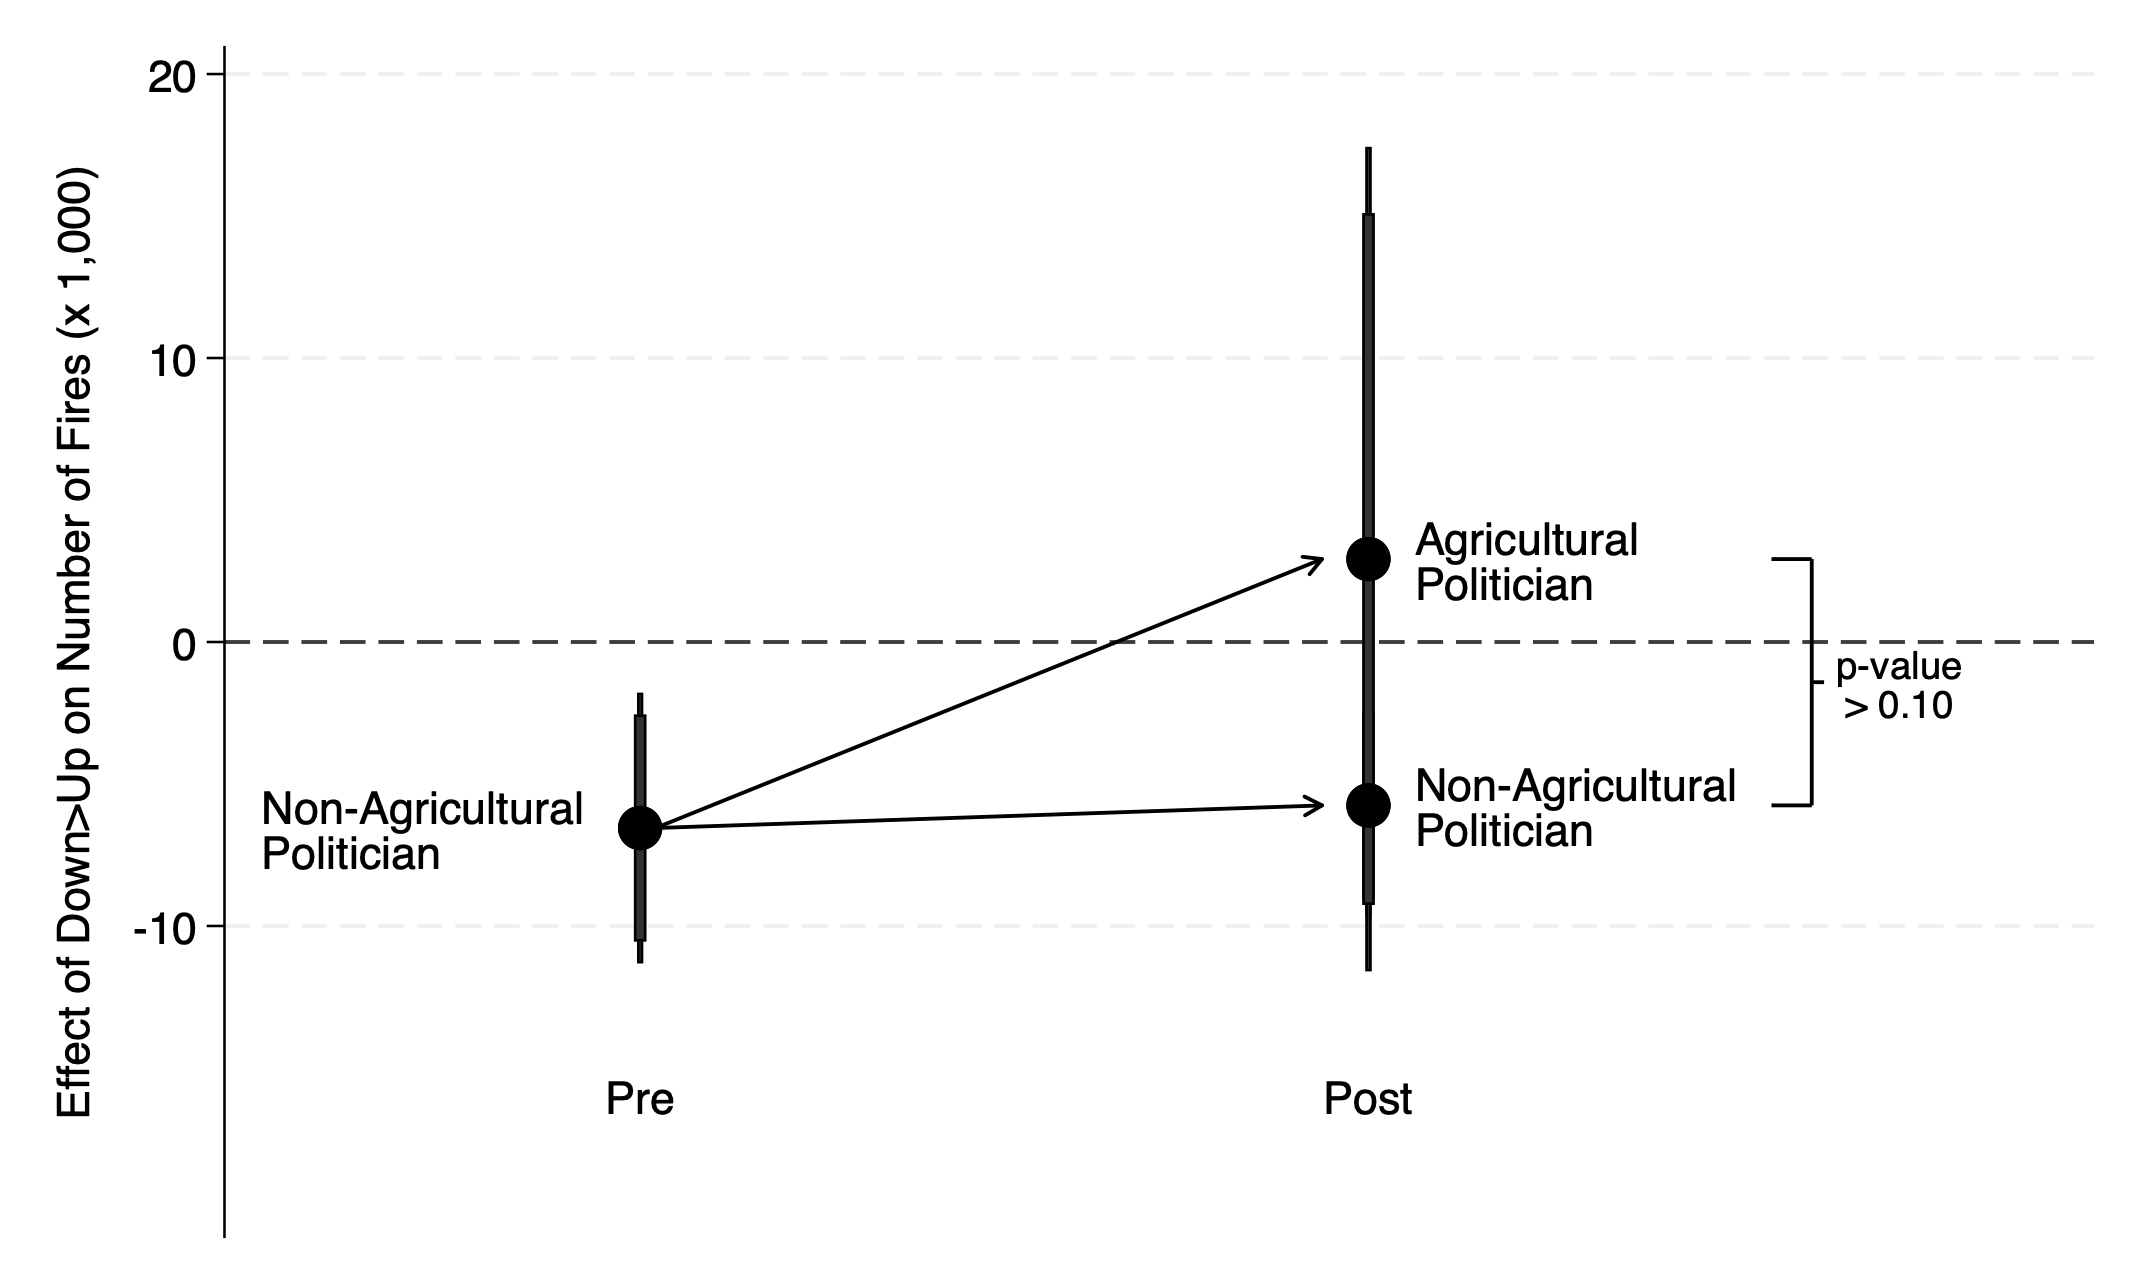
\includegraphics[width=0.85\linewidth]{../figures/app19_polischar_did_downup_1.png}
\caption{Polischar $\times$ downup\_ac (fe1)}
\end{figure}
\subsection*{FE specification \texttt{fe8} (slot `evreg2')}
\begin{figure}[H]
\centering
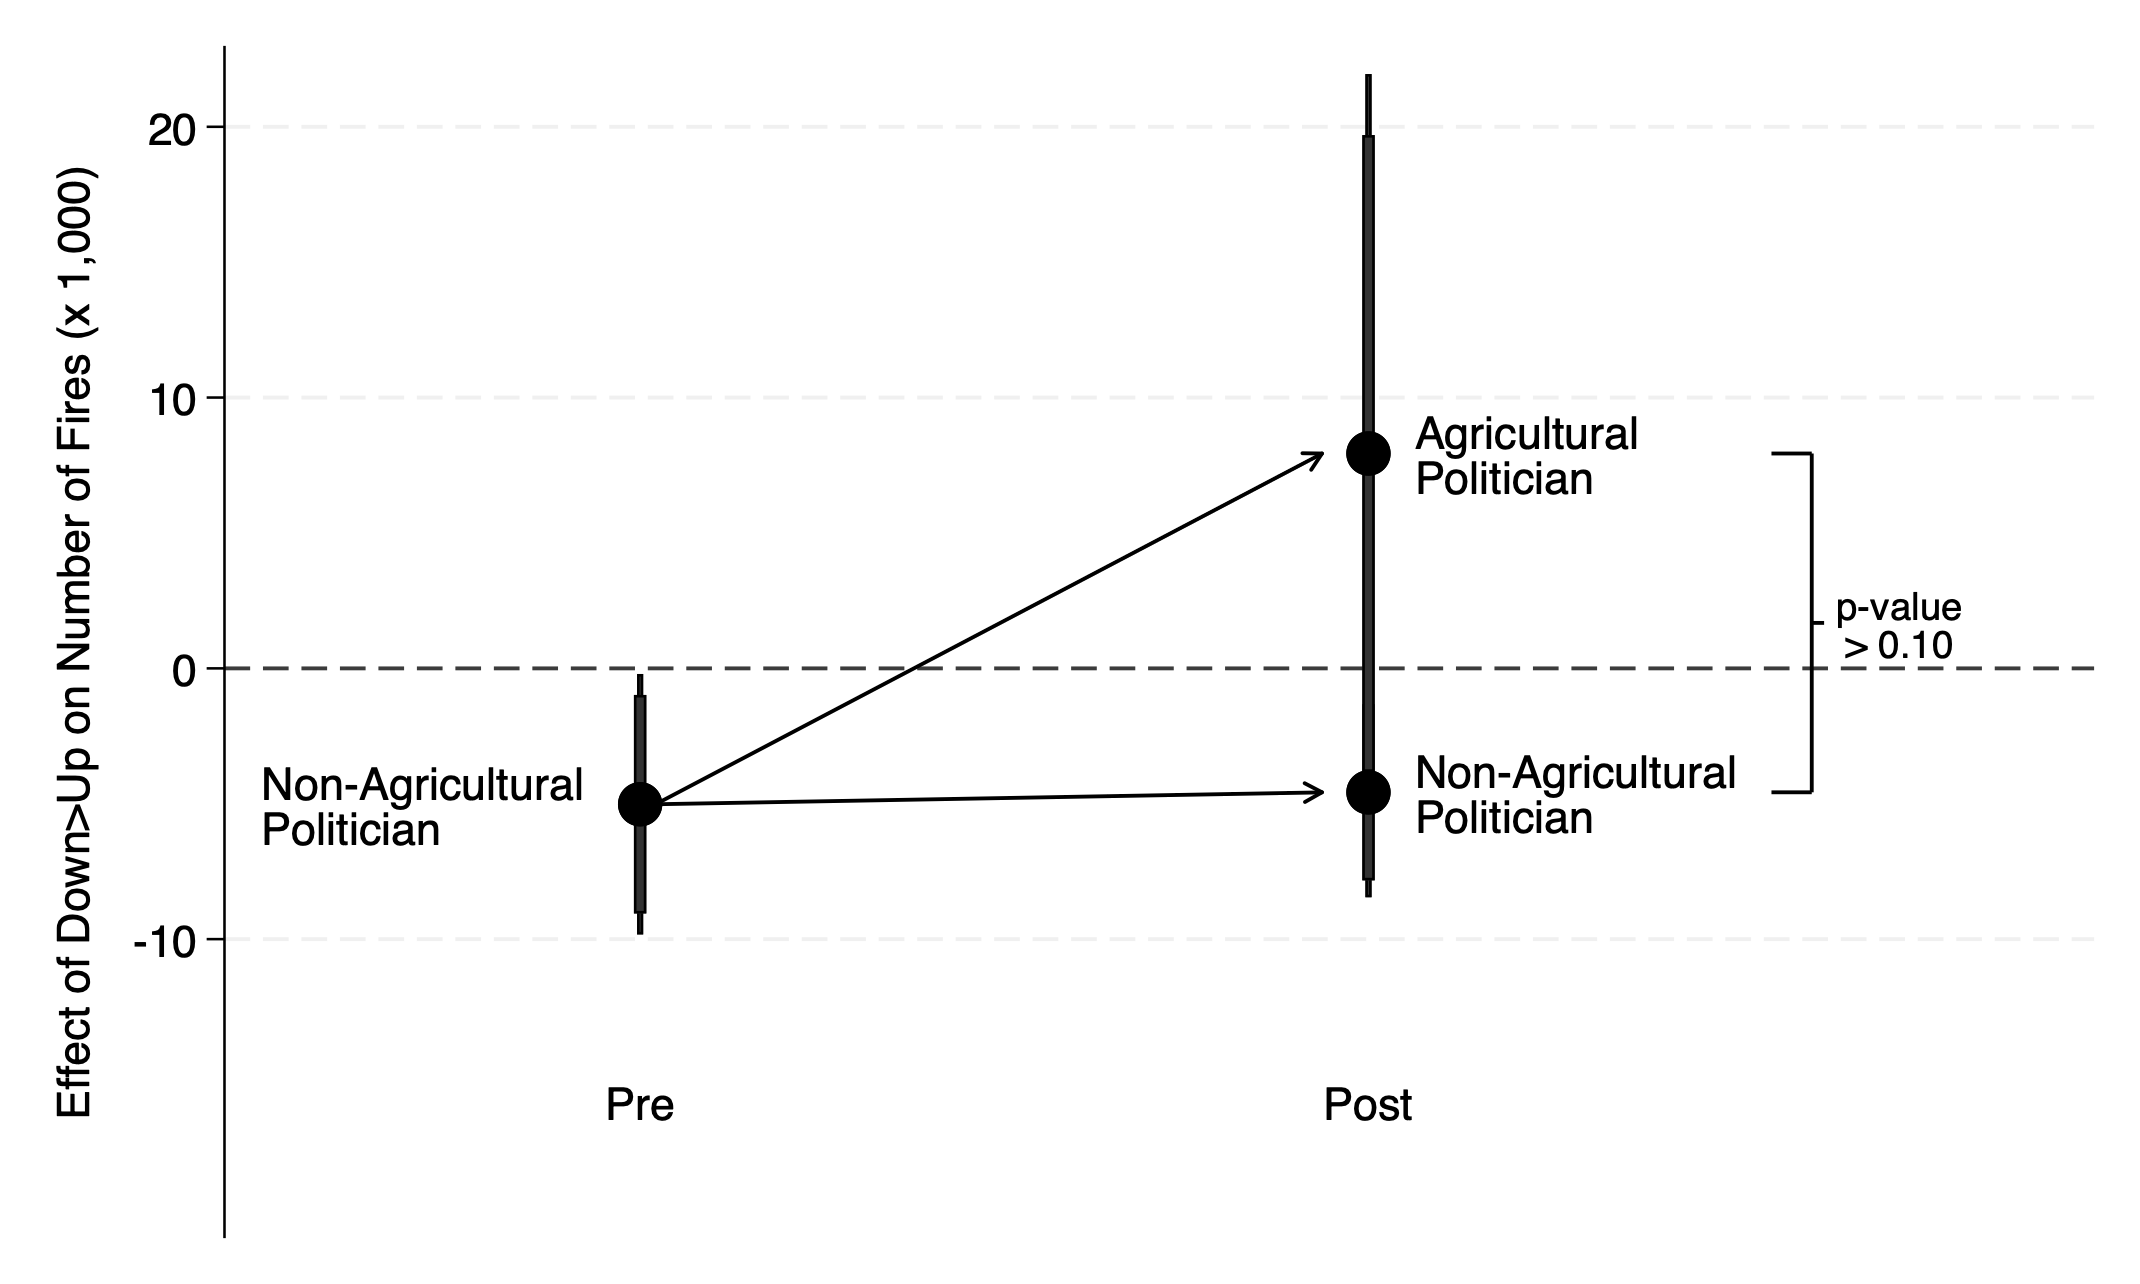
\includegraphics[width=0.85\linewidth]{../figures/app19_polischar_did_downup_2.png}
\caption{Polischar $\times$ downup\_ac (fe8)}
\end{figure}
\subsection*{FE specification \texttt{fe16} (slot `evreg3')}
\begin{figure}[H]
\centering
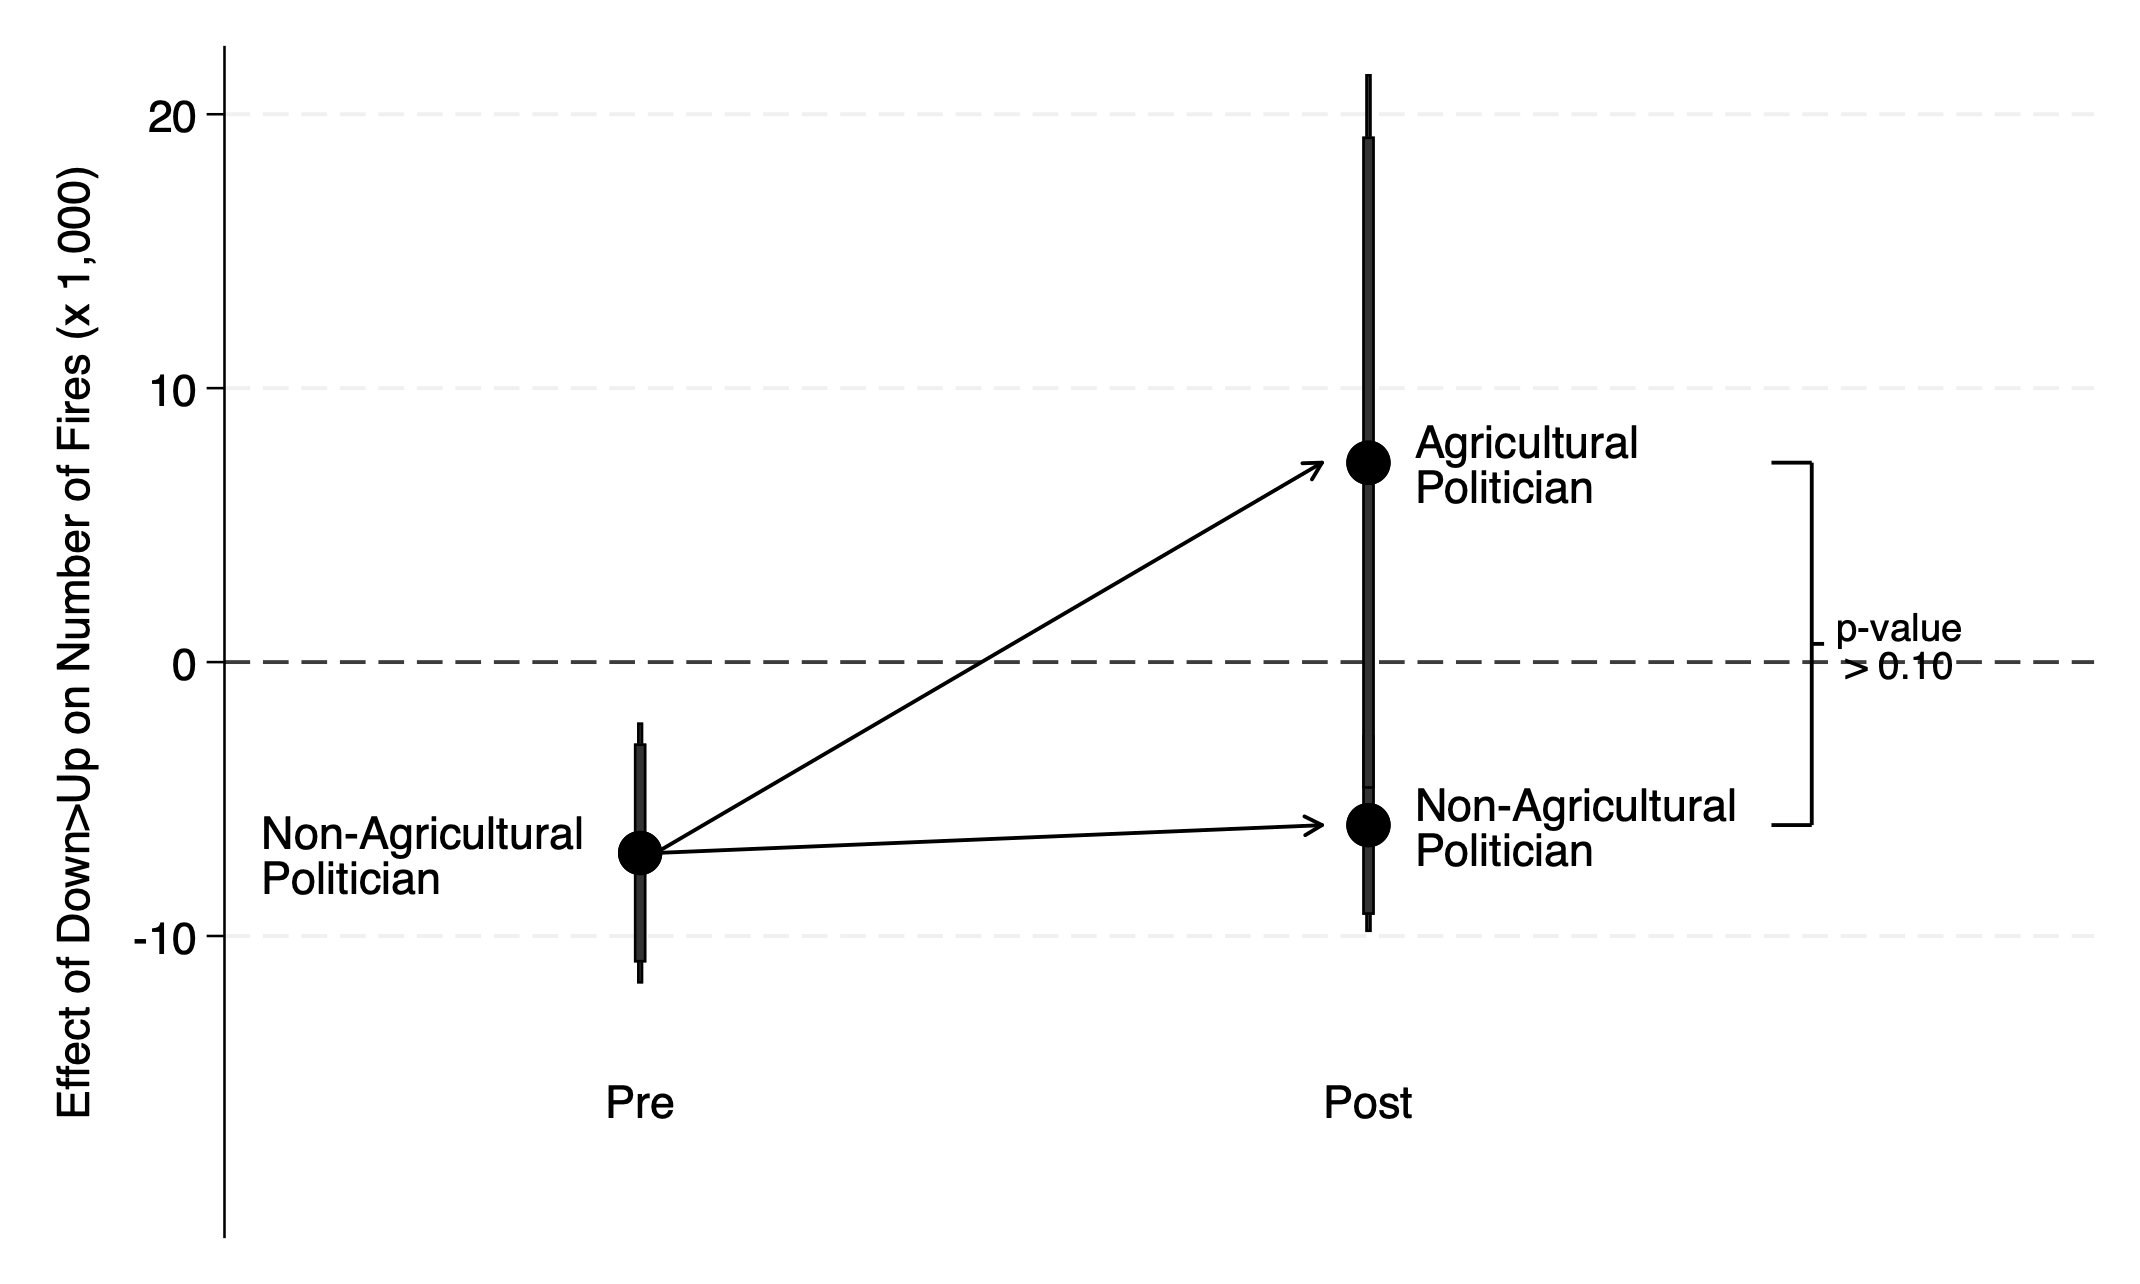
\includegraphics[width=0.85\linewidth]{../figures/app19_polischar_did_downup_3.png}
\caption{Polischar $\times$ downup\_ac (fe16)}
\end{figure}
\subsection*{FE specification \texttt{fe24} (slot `evreg4')}
\begin{figure}[H]
\centering
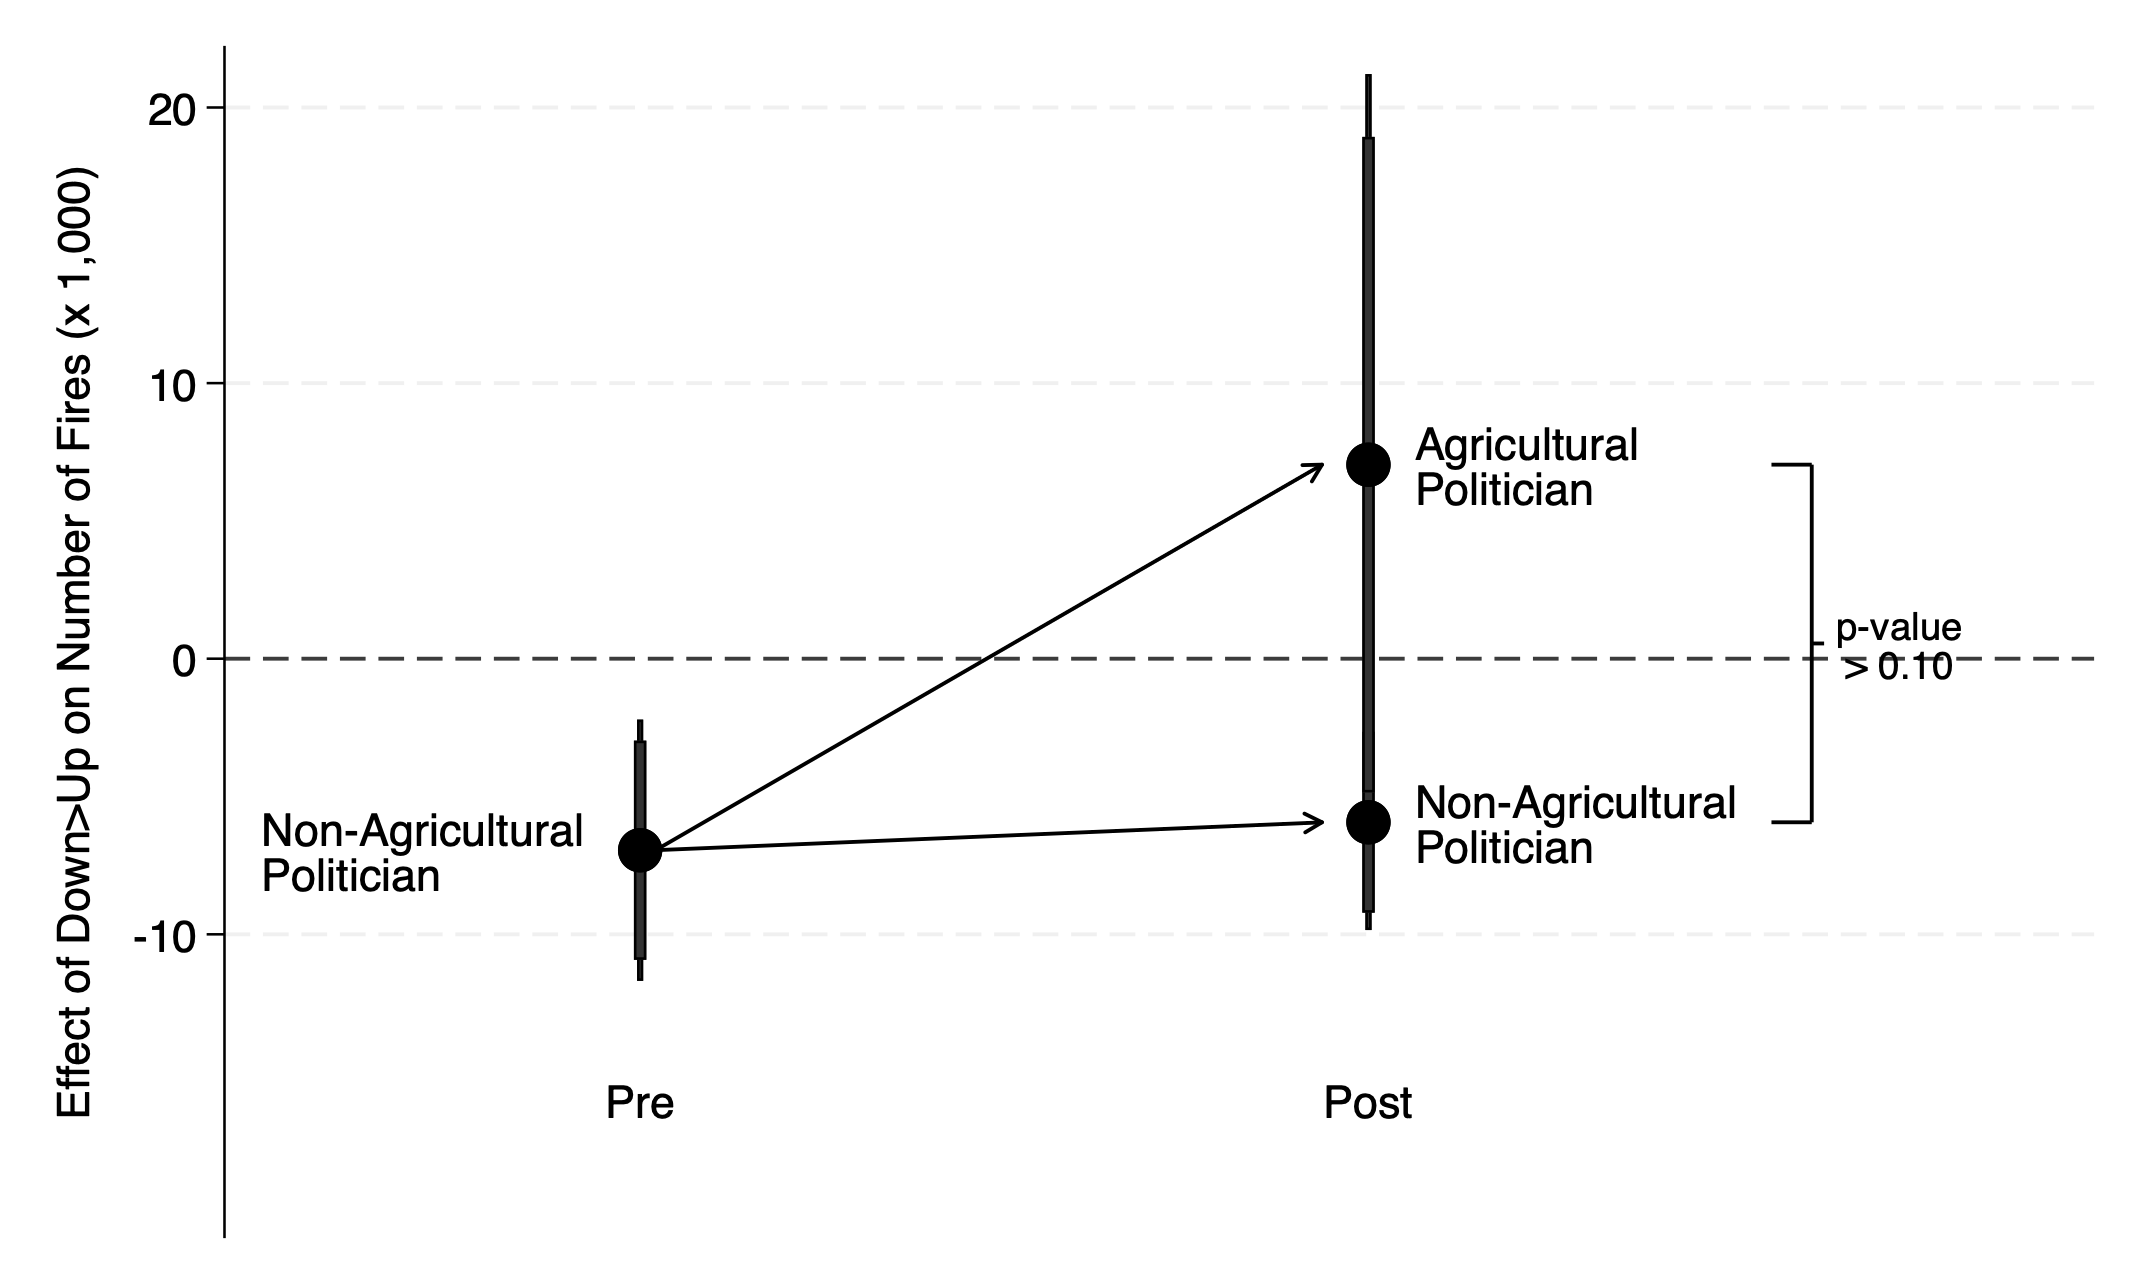
\includegraphics[width=0.85\linewidth]{../figures/app19_polischar_did_downup_4.png}
\caption{Polischar $\times$ downup\_ac (fe24)}
\end{figure}
\subsection*{FE specification \texttt{fe32} (slot `evreg5')}
\begin{figure}[H]
\centering
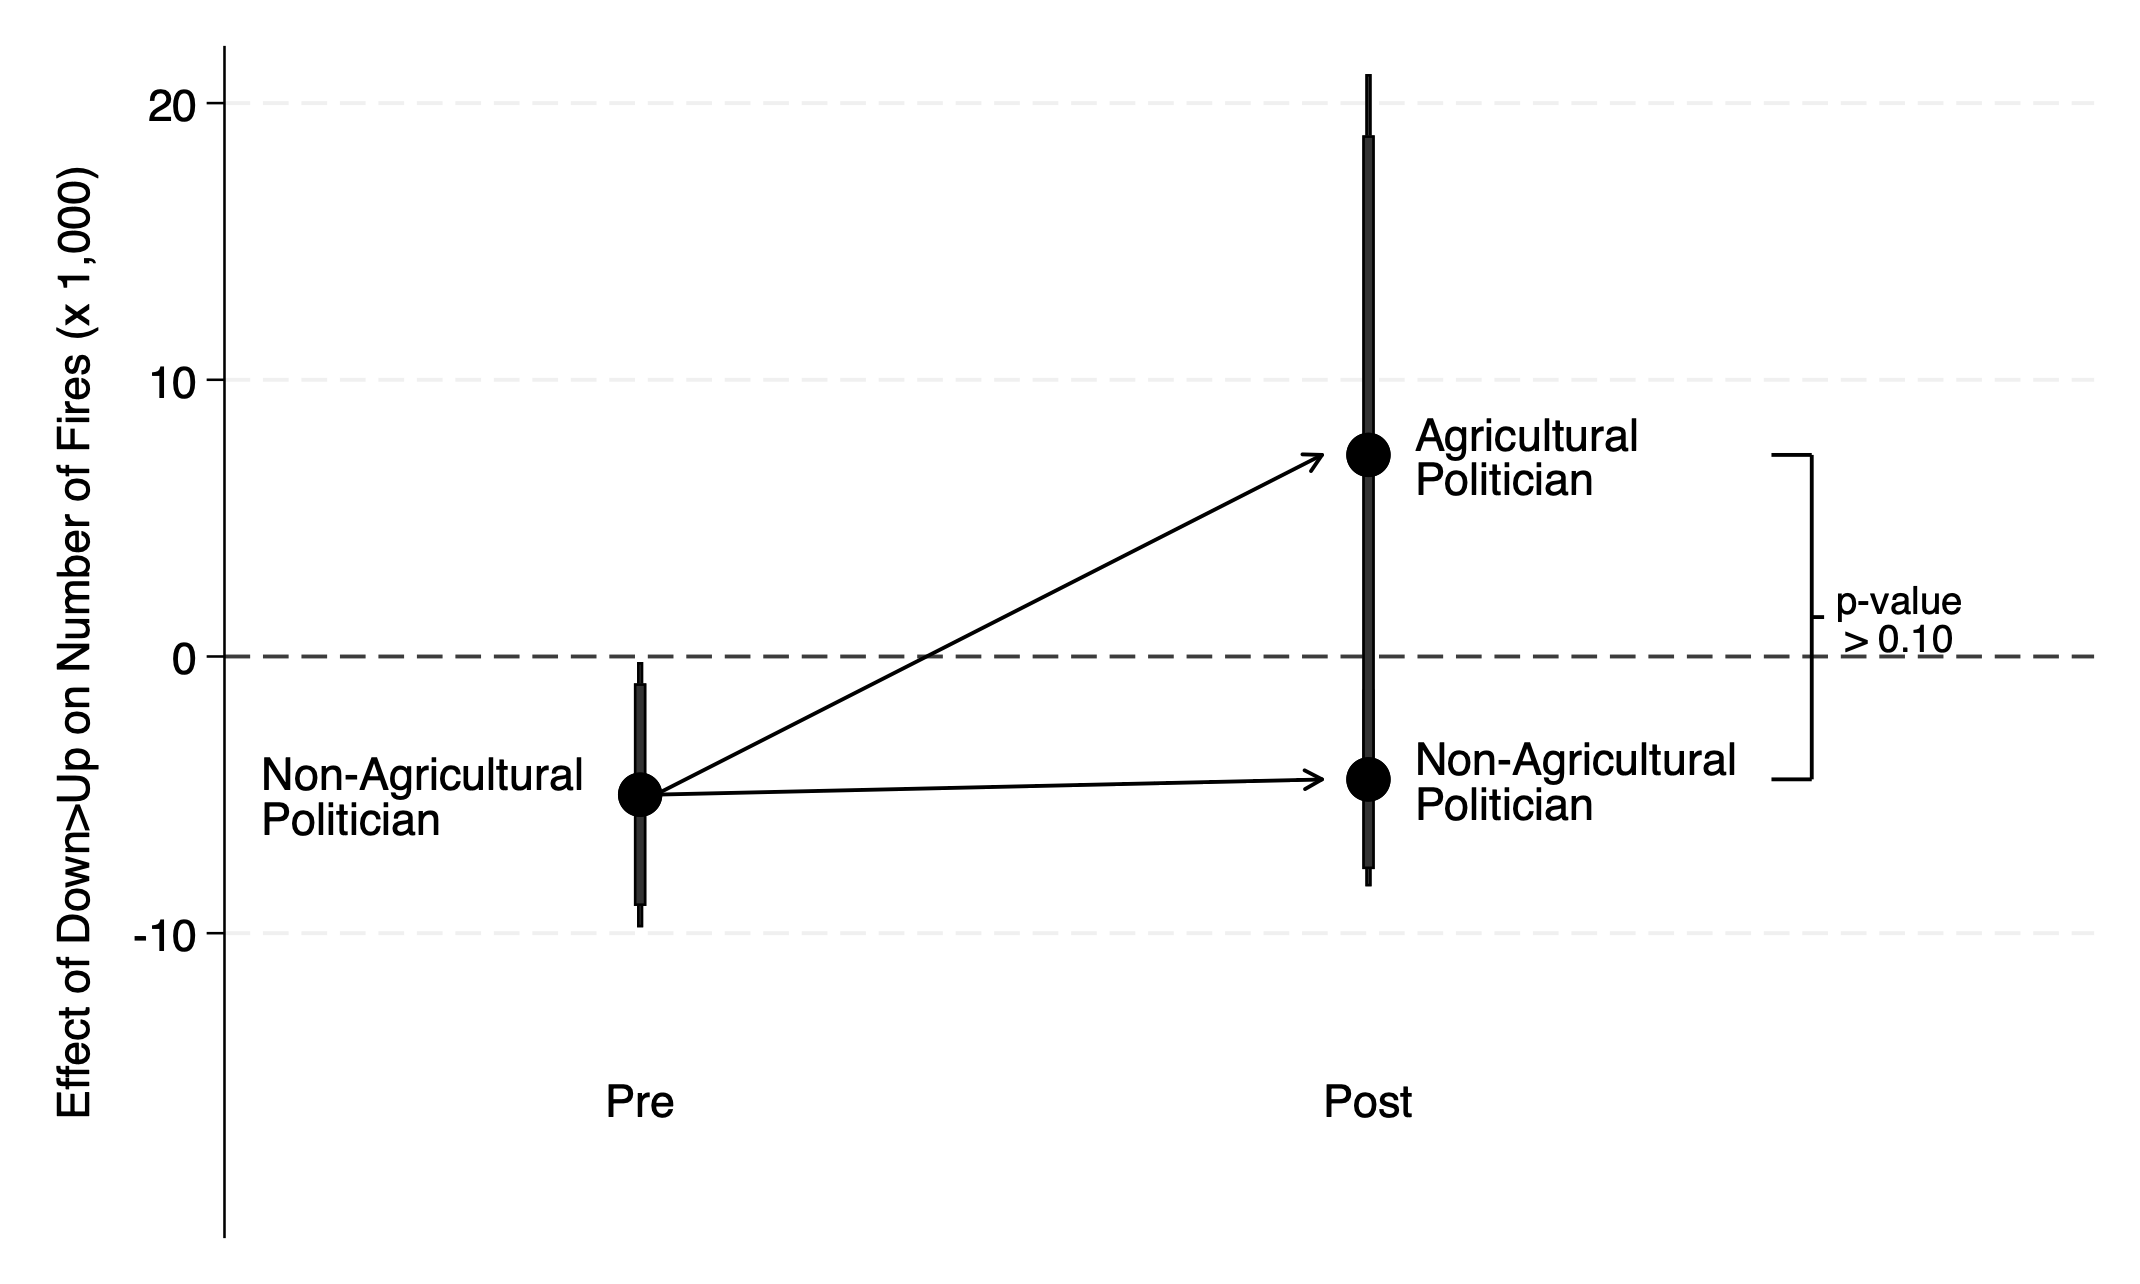
\includegraphics[width=0.85\linewidth]{../figures/app19_polischar_did_downup_5.png}
\caption{Polischar $\times$ downup\_ac (fe32)}
\end{figure}
\FloatBarrier

\end{document}
